% BigMath: How the Algorithms Work — A Practitioner's Guide
%
% Build (from this directory):
%   python3 figures/make_figures.py      # only when thresholds/measurements change
%   latexmk -pdf algorithms-guide.tex    # or: pdflatex x3
%
\documentclass[11pt,a4paper,oneside]{report}

\usepackage[T1]{fontenc}
\usepackage[utf8]{inputenc}
\usepackage{lmodern}
\usepackage{microtype}
\usepackage[margin=2.5cm,headheight=14pt]{geometry}
\usepackage{amsmath,amssymb,mathtools}
\usepackage{xcolor}
\usepackage{graphicx}
\usepackage{booktabs,array,tabularx,multirow,longtable}
\usepackage{enumitem}
\usepackage{caption}
\usepackage{float}
\usepackage{fancyhdr}
\usepackage{listings}
\usepackage{tikz}
\usetikzlibrary{calc,positioning,arrows.meta,decorations.pathreplacing,matrix,fit,shapes.geometric,shapes.misc,backgrounds}
\usepackage{tcolorbox}
\tcbuselibrary{skins,breakable}
\usepackage[hidelinks]{hyperref}
\usepackage{cleveref}

% ---------------------------------------------------------------- colours
\definecolor{sBlue}{HTML}{2A78D6}
\definecolor{sOrange}{HTML}{EB6834}
\definecolor{sAqua}{HTML}{1BAF7A}
\definecolor{sYellow}{HTML}{EDA100}
\definecolor{sMagenta}{HTML}{E87BA4}
\definecolor{sGreen}{HTML}{008300}
\definecolor{sViolet}{HTML}{6250D6}
\definecolor{sRed}{HTML}{E34948}
\definecolor{ink}{HTML}{0B0B0B}
\definecolor{ink2}{HTML}{52514E}
\definecolor{muted}{HTML}{8A8984}
\definecolor{paper}{HTML}{F6F5F2}
\definecolor{rule}{HTML}{E4E3DF}

% ---------------------------------------------------------------- boxes
\tcbset{guidebox/.style={enhanced,breakable,boxrule=0pt,leftrule=3pt,arc=1pt,
  left=8pt,right=8pt,top=5pt,bottom=5pt,fonttitle=\bfseries\small,
  coltitle=ink,colback=paper,attach title to upper,after title={\quad}}}
\newtcolorbox{keyidea}[1][]{guidebox,colframe=sBlue,title={Key idea#1}}
\newtcolorbox{example}[1][]{guidebox,colframe=sAqua,title={Worked example#1}}
\newtcolorbox{perfnote}[1][]{guidebox,colframe=sOrange,title={Why it is fast#1}}
\newtcolorbox{another}[1][]{guidebox,colframe=sViolet,title={Another way to see it#1}}
\newtcolorbox{practice}[1][]{guidebox,colframe=sGreen,title={What this means for you#1}}
\newtcolorbox{pitfall}[1][]{guidebox,colframe=sRed,title={Lesson learned#1}}

% ---------------------------------------------------------------- code
\lstdefinestyle{cpp}{language=C++,basicstyle=\ttfamily\small,keywordstyle=\color{sBlue}\bfseries,
  commentstyle=\color{ink2}\itshape,stringstyle=\color{sOrange},showstringspaces=false,
  columns=fullflexible,keepspaces=true,frame=single,rulecolor=\color{rule},
  backgroundcolor=\color{paper},xleftmargin=4pt,xrightmargin=4pt,framesep=4pt,breaklines=true}
\lstdefinestyle{pseudo}{basicstyle=\ttfamily\small,columns=fullflexible,keepspaces=true,
  frame=single,rulecolor=\color{rule},backgroundcolor=\color{paper},xleftmargin=4pt,
  xrightmargin=4pt,framesep=4pt,mathescape=true,breaklines=true}
\lstset{style=cpp}

% ---------------------------------------------------------------- macros
% Inline code and paths: allow line breaks after underscores and slashes.
\newcommand{\brkus}{\textunderscore\allowbreak}
\newcommand{\brksl}{/\allowbreak}
\DeclareRobustCommand{\code}[1]{\begingroup\small\ttfamily\let\_\brkus#1\endgroup}
\ExplSyntaxOn
\tl_new:N \l__guide_path_tl
\NewDocumentCommand{\file}{m}{
  \group_begin:
  \small\ttfamily
  \let\_\brkus
  \tl_set:Nn \l__guide_path_tl {#1}
  \tl_replace_all:Nnn \l__guide_path_tl {/} {\brksl}
  \tl_use:N \l__guide_path_tl
  \group_end:
}
\ExplSyntaxOff
\newcommand{\B}{\ensuremath{B}}
\newcommand{\M}{\ensuremath{\mathsf{M}}}
\newcommand{\bigO}{\ensuremath{O}}
\newcommand{\floor}[1]{\left\lfloor #1 \right\rfloor}
\newcommand{\ceil}[1]{\left\lceil #1 \right\rceil}
\newcommand{\algo}[1]{\textsf{#1}}

% TikZ styles shared by all figures
\tikzset{
  limb/.style={draw=ink2,minimum width=12mm,minimum height=6mm,font=\small\ttfamily,fill=white},
  box/.style={draw=ink2,rounded corners=2pt,align=center,font=\small,fill=white,inner sep=4pt},
  dec/.style={draw=ink2,diamond,aspect=2.2,align=center,font=\footnotesize,fill=paper,inner sep=1pt},
  algo/.style={draw=none,rounded corners=2pt,align=center,font=\small\bfseries,text=white,inner sep=4pt},
  arr/.style={-{Stealth[length=2mm]},draw=ink2,thick},
  lbl/.style={font=\footnotesize,text=ink2},
}

\captionsetup{font=small,labelfont=bf}
\setlist{itemsep=2pt,topsep=4pt}
\setlength{\parskip}{4pt}
\setlength{\parindent}{0pt}
\setlength{\emergencystretch}{2em}

\pagestyle{fancy}
\fancyhf{}
\fancyhead[L]{\small\color{ink2}\leftmark}

\fancyfoot[C]{\small\thepage}
\renewcommand{\headrulewidth}{0.4pt}

\newcommand{\guideauthor}{S M Mahbub Murshed}
\newcommand{\guideauthoremail}{murshed@gmail.com}
\hypersetup{pdftitle={BigMath: How the Algorithms Work},pdfauthor={\guideauthor}}

\begin{document}

\hypersetup{pageanchor=false}
\begin{titlepage}
  \centering
  \vspace*{3cm}
  {\Huge\bfseries BigMath\par}
  \vspace{0.6cm}
  {\LARGE How the Algorithms Work\par}
  \vspace{0.4cm}
  {\large A practitioner's guide to the arithmetic inside the library,\\
  when each algorithm runs, and why\par}
  \vspace{0.8cm}
  {\large \guideauthor\par}
  \smallskip
  {\small \href{mailto:\guideauthoremail}{\guideauthoremail}\par}
  \vspace{2cm}
  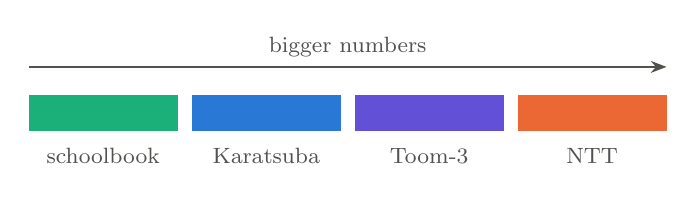
\begin{tikzpicture}[scale=0.9]
    \foreach \x/\c/\t in {0/sAqua/schoolbook,1/sBlue/Karatsuba,2/sViolet/Toom-3,3/sOrange/NTT} {
      \fill[\c] (\x*2.3,0) rectangle +(2.1,0.5);
      \node[lbl] at (\x*2.3+1.05,-0.35) {\t};
    }
    \draw[arr] (0,0.9) -- node[above,lbl]{bigger numbers} (9.0,0.9);
  \end{tikzpicture}
  \vfill
  {\small Covers the 64-bit build with the CRT number-theoretic transform and internal
  thread pool. Includes generic thresholds, checked-in platform profiles, and
  November 2026 measurements from an Apple M1 Max.\par}
  \vspace{0.5cm}
  {\small Source: \file{docs/algorithms-guide/}\par}
\end{titlepage}
\hypersetup{pageanchor=true}

\tableofcontents

\chapter{Start here}
\label{ch:start}

\section{Who this guide is for}

You want to use BigMath to work with integers that are too big for a machine word:
cryptographic sizes, exact combinatorics, computing millions of digits of a constant,
or a calculator that never overflows. You do not need to know how big-number
arithmetic works inside. But knowing it helps you predict how long an operation will
take, pick the right API, and understand what the build options do.

This guide explains every algorithm the library uses, in plain language. Each one is
explained in more than one way: a picture, a small example you can check by hand,
and the reason it is faster than the simpler method. It also explains \emph{when} the
library switches from one algorithm to another, and why the switch points sit where
they do.

You will not need more mathematics than school algebra. Where a formula appears, the
text around it says in words what it means.

\section{How to read it}

The chapters build on each other, but you can jump around:

\begin{itemize}
  \item \Cref{ch:repr,ch:basics} cover how numbers are stored and how the small
        building blocks (add, subtract, multiply by one limb) work. Everything
        else is made of these.
  \item \Cref{ch:mul,ch:ntt,ch:fermat} explain multiplication from schoolbook
        through the NTT and the experimental Fermat FFT. See \cref{ch:muldispatch}
        for the dispatch rules.
  \item \Cref{ch:div,ch:fastdiv,ch:divdispatch} cover division, including
        Hensel exact division (\cref{sec:exactdivision}).
  \item \Cref{ch:conv} covers decimal strings, radix conversion (\cref{sec:convertbase}),
        and fixed-point arithmetic.
  \item \Cref{ch:numbertheory} covers GCD, integer roots, modular powers, prime
        searches, combinatorics, and reconstruction from modular residues.
  \item \Cref{ch:parallel} covers the thread pool.
  \item \Cref{ch:practice} is a checklist for using the library well, and
        \cref{ch:decisions} records the ideas that were tried and rejected.
  \item \Cref{app:ref} lists every threshold in one place.
\end{itemize}

Six kinds of boxes appear throughout:

\begin{keyidea}
The one sentence to remember about a section.
\end{keyidea}
\begin{example}
A small calculation you can follow with pencil and paper.
\end{example}
\begin{another}
The same idea explained from a different angle.
\end{another}
\begin{perfnote}
What makes the method fast on a real processor.
\end{perfnote}
\begin{practice}
Advice for someone calling the library.
\end{practice}
\begin{pitfall}
Something that went wrong during development, and what it taught.
\end{pitfall}

\section{Words used in this guide}

\begin{description}[leftmargin=2.2cm,style=nextline]
  \item[limb] One machine word of a big number. BigMath limbs are 64 bits wide,
        so a limb holds a ``digit'' between $0$ and $2^{64}-1$. A 1000-digit decimal
        number needs about 52 limbs.
  \item[$B$] The base of the limbs, $B = 2^{64}$. A number with limbs
        $a_0, a_1, \dots, a_{n-1}$ has the value
        $a_0 + a_1 B + a_2 B^2 + \dots + a_{n-1}B^{n-1}$.
  \item[$n$, $n_a$, $n_b$] Lengths in limbs.
  \item[$\M(n)$] The time to multiply two $n$-limb numbers. Division and
        conversion are often described as ``a few $\M(n)$''.
  \item[threshold] A size at which the library switches algorithm. All
        thresholds were measured, not guessed (\cref{sec:measured}).
  \item[dispatcher] The function that looks at the operand sizes and picks the
        algorithm.
  \item[warm / cold pool] Whether the worker threads are awake (warm) or asleep
        (cold) when an operation starts. See \cref{ch:parallel}.
\end{description}

As a rule of thumb, one limb is about 19.3 decimal digits:

\begin{center}
\begin{tabular}{rrr}
\toprule
decimal digits & bits & limbs \\
\midrule
100 & 333 & 6 \\
1\,000 & 3\,322 & 52 \\
10\,000 & 33\,220 & 520 \\
1\,000\,000 & 3.3 million & 52\,000 \\
100\,000\,000 & 332 million & 5.2 million \\
\bottomrule
\end{tabular}
\end{center}

\section{The whole library on one page}
\label{sec:onepage}

\Cref{tab:onepage} is the short version of this guide. For each operation it shows
which algorithm runs at which size with the generic thresholds. Sizes are in
limbs unless marked as bits or decimal digits. Platform profiles can override the thresholds
(\cref{sec:platformprofiles}).

\begin{table}[!t]
\centering
\small
\renewcommand{\arraystretch}{1.10}
\begin{tabularx}{\textwidth}{@{}l l >{\raggedright\arraybackslash}X@{}}
\toprule
operation & size (limbs) & algorithm \\
\midrule
$a \pm b$ & any & serial carry or borrow chain (\cref{sec:paralleladdsub}) \\
\midrule
\multirow{5}{*}{$a \times b$}
  & both $\le 16$ & stack-buffer schoolbook (\cref{sec:smallops}) \\
  & shorter $\le 24$, or total $\le 56$ & schoolbook (\cref{sec:schoolbook}) \\
  & up to $\approx 310$ each & Karatsuba; levels with $\ge 168$ limbs split three ways (Toom-3) (\cref{sec:karatsuba,sec:toom}) \\
  & shorter $\ge 64$, area $\ge 96\,000$ & NTT if the thread pool is awake, else Karatsuba (\cref{sec:poolrule}) \\
  & area $\ge 262\,144$ ($\approx 512\times512$) & NTT always (\cref{ch:ntt}) \\
\midrule
\multirow{3}{*}{$a^2$}
  & $< 352$ & Karatsuba square (Toom-3 from 160) \\
  & $352$--$607$ & NTT if pool awake, else Karatsuba square \\
  & $\ge 608$ & NTT (only three forward transforms) \\
\midrule
\multirow{5}{*}{$a \div b$}
  & divisor 1 limb & short division with a precomputed reciprocal (\cref{sec:shortdiv}) \\
  & divisor $< 96$ & schoolbook long division, Knuth's Algorithm D (\cref{sec:knuth}) \\
  & quotient $\ge$ divisor & Burnikel--Ziegler, or Newton from divisor 1536 (768 if ratio $\ge 3$) \\
  & quotient $<$ divisor & Burnikel--Ziegler; Newton from 3072 at ratio $\ge 7/4$; quotient-sized if the quotient has $\ge 3072$ limbs \\
  & \code{a / b} with short quotient & divide only the top limbs (\cref{sec:toplimbs}) \\
\midrule
parse & $\le 2048$ digits & 18 digits at a time, multiply-and-add (\cref{sec:linparse}) \\
      & larger & split in half, recurse, combine with one multiply; 8 threads from 100\,000 digits \\
\midrule
format & standalone 48--96 & scaled-remainder chunk extraction (\cref{sec:scaledformat}) \\
       & other inputs $<1024$ digits & direct for one limb; 19-digit short division otherwise \\
       & larger inputs & split by powers of ten; scaled or scalar leaves \\
\midrule
GCD & shorter $\ge 65\,536$ bits & half-GCD for comparable widths; extended cutoff 16\,384 bits (\cref{sec:halfgcd}) \\
modular power & odd modulus $\ge 64$ & FastREDC with exponents from 64 bits (\cref{sec:fastredc}) \\
\bottomrule
\end{tabularx}
\caption{Arithmetic dispatch with generic thresholds and 64-bit limbs.}
\label{tab:onepage}
\end{table}

\section{Why the switch points are measured}
\label{sec:measured}

Textbooks say ``Karatsuba is faster than schoolbook for large $n$''. That is true but
not useful: \emph{how} large? The answer depends on the processor, the compiler, and
how carefully each algorithm is written. A clever algorithm has extra bookkeeping. It
only wins once the numbers are big enough for the savings to pay for that bookkeeping.

BigMath measures crossovers on a grid of sizes and shapes. The generic
thresholds come from \file{include/biginteger/build/DispatchThresholds.h}.
A platform profile supplies overrides for its compiler and target. You
can also override individual thresholds at build time, for example with
\code{-DBIGMATH\_KARATSUBA\_THRESHOLD=32}. The timing examples in this
guide are measurements from an Apple M1 Max. Crossovers depend on the
target CPU, compiler, and worker state.

\begin{keyidea}
An algorithm with a better growth rate always wins eventually, but ``eventually'' is
a number that has to be measured. BigMath uses the simplest method that is fastest at
each size, and switches at measured crossover points.
\end{keyidea}

\chapter{How a big number is stored}
\label{ch:repr}

\section{Limbs: digits in base $2^{64}$}

On paper we write numbers in base 10: each digit is $0$--$9$ and each position is
worth ten times the one to its right. A computer can do the same thing with a much
bigger base. BigMath uses base $B = 2^{64}$: each ``digit'', called a \emph{limb}, is a
whole 64-bit machine word and can be anything from $0$ to
$18\,446\,744\,073\,709\,551\,615$.

\begin{keyidea}
A \code{BigInteger} is a list of 64-bit limbs plus a sign. The value is
$a_0 + a_1 B + a_2 B^2 + \dots$ with $B = 2^{64}$: exactly like decimal digits, but each
``digit'' is a 64-bit word.
\end{keyidea}

The limbs are stored \emph{little-endian}: the least significant limb comes first,
at index 0.

\begin{figure}[ht]
\centering
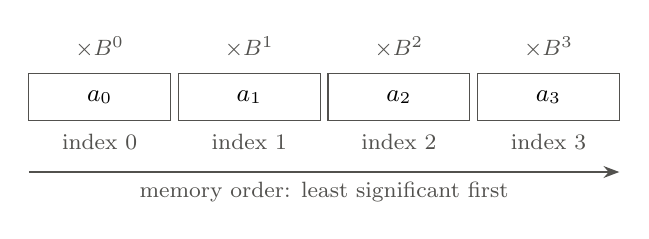
\begin{tikzpicture}
  \foreach \i/\v in {0/a_0,1/a_1,2/a_2,3/a_3} {
    \node[limb,minimum width=18mm] (L\i) at (\i*1.9,0) {$\v$};
    \node[lbl,below=1pt of L\i] {index \i};
  }
  \node[lbl,above=2pt of L0] {$\times B^0$};
  \node[lbl,above=2pt of L1] {$\times B^1$};
  \node[lbl,above=2pt of L2] {$\times B^2$};
  \node[lbl,above=2pt of L3] {$\times B^3$};
  \draw[arr] (-0.9,-0.95) -- node[below,lbl]{memory order: least significant first} (6.6,-0.95);
\end{tikzpicture}
\caption{A four-limb number in memory. Limb $i$ is worth $B^i = 2^{64 i}$.}
\label{fig:limbs}
\end{figure}

\begin{example}[: writing $2^{130} + 5$ in limbs]
Divide by $B = 2^{64}$ repeatedly, as you would to convert to any base:
\begin{itemize}
  \item $2^{130} + 5 = 2^{66}\cdot B + 5$, so $a_0 = 5$ and the rest is $2^{66}$.
  \item $2^{66} = 4 \cdot B + 0$, so $a_1 = 0$ and the rest is $4$.
  \item $4 < B$, so $a_2 = 4$.
\end{itemize}
The limbs are $[5,\ 0,\ 4]$. Check: $5 + 0\cdot 2^{64} + 4 \cdot 2^{128} = 2^{130} + 5$.
\end{example}

\subsection{Why base $2^{64}$?}

\begin{itemize}
  \item \textbf{The hardware already does it.} A 64-bit processor multiplies two
        64-bit words and returns the full 128-bit result in one or two
        instructions (\code{MUL}+\code{UMULH} on ARM, \code{MUL} on x86). So a
        limb-by-limb product is as cheap as it can be.
  \item \textbf{Fewer limbs means less work.} Many algorithms cost about $n^2$
        limb operations for $n$-limb inputs. Halving the number of limbs
        (base $2^{64}$ instead of $2^{32}$) quarters that work. The library used
        32-bit values in 64-bit slots for years; moving to full 64-bit limbs was
        the biggest single speedup in its history. The old layout is still
        available with \code{-DBIGMATH\_LIMB\_64=0} for comparison.
  \item \textbf{Binary operations are free.} Shifts, bit tests, and conversion
        to hexadecimal work directly on the stored bits.
\end{itemize}

The price is decimal conversion: turning limbs into decimal digits is real work
(\cref{ch:conv}). Storing numbers in base $10^{18}$ would make printing trivial but
every arithmetic operation slower; arithmetic happens far more often than printing.

\subsection{Why little-endian?}

Carries flow from the least significant limb to the most significant. With the low
limb at index 0, every loop runs forward through memory, which is what processors
prefetch best. A result that grows by one limb (a final carry) just gets one more
element appended at the end; nothing has to move.

\section{Sign and magnitude}

The sign is stored separately as a flag; the limbs hold the absolute value. So $-5$ is
the limbs $[5]$ with the sign flag set. Algorithms work on the magnitudes and the
operator layer (\file{include/biginteger/ops/}) works out the sign of the result:
for example, the product is negative when exactly one input is negative.

Division truncates toward zero, as in C and C++: the quotient is rounded toward zero
and the remainder has the sign of the dividend.

\begin{center}
\begin{tabular}{rrrr}
\toprule
$a$ & $b$ & $a / b$ & $a \% b$ \\
\midrule
$7$ & $2$ & $3$ & $1$ \\
$-7$ & $2$ & $-3$ & $-1$ \\
$7$ & $-2$ & $-3$ & $1$ \\
$-7$ & $-2$ & $3$ & $-1$ \\
\bottomrule
\end{tabular}
\end{center}

In every row $b \cdot (a/b) + (a \% b) = a$.

\section{Small numbers stay inside the object}
\label{sec:smallops}

Most programs that use big integers also use many \emph{small} ones: counters,
loop bounds, intermediate values that happen to be short. If every value needed a
heap allocation, copying the number $3$ would cost as much as calling \code{malloc}.

BigMath therefore keeps numbers of up to four limbs (256 bits,
\code{BIGMATH\_INLINE\_LIMBS}) \emph{inside} the \code{BigInteger} object. Only longer
numbers use a \code{std::vector}. The rule is strict: after trimming leading zero
limbs, a value is stored inline exactly when it has at most four limbs. So copying a
small value never allocates.

\begin{figure}[ht]
\centering
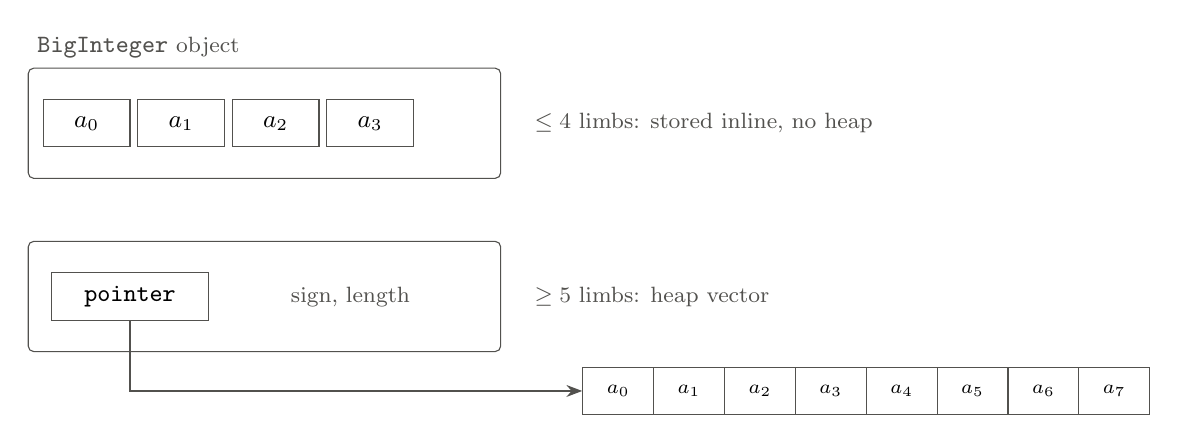
\begin{tikzpicture}
  \node[box,minimum width=60mm,minimum height=14mm,anchor=west] (obj) at (0,0) {};
  \node[lbl,anchor=south west] at (obj.north west) {\code{BigInteger} object};
  \foreach \i in {0,1,2,3} \node[limb,minimum width=11mm] at (0.75+\i*1.2,0) {$a_\i$};
  \node[lbl,anchor=west] at (obj.east) {\quad $\le 4$ limbs: stored inline, no heap};
  \node[box,minimum width=60mm,minimum height=14mm,anchor=west] (obj2) at (0,-2.2) {};
  \node[limb,minimum width=20mm] (p) at (1.3,-2.2) {pointer};
  \node[lbl] at (4.1,-2.2) {sign, length};
  \foreach \i in {0,...,7} \node[limb,minimum width=9mm] (h\i) at (7.5+\i*0.9,-3.4) {\scriptsize$a_{\i}$};
  \draw[arr] (p.south) |- (h0.west);
  \node[lbl,anchor=west] at (obj2.east) {\quad $\ge 5$ limbs: heap vector};
\end{tikzpicture}
\caption{Inline storage for short values, heap storage for long ones.}
\end{figure}

The operators go one step further. When both operands have at most 16 limbs
(\code{BIGMATH\_SMALL\_OPS\_MAX\_LIMBS}), \code{+}, \code{-}, \code{*}, \code{/}
and \code{\%} compute the result in a buffer on the stack using the limb kernels of
\cref{ch:basics}, then build the result object directly. No temporary vectors are
created; the only possible allocation is the result itself when it has more than four
limbs.

\begin{perfnote}
Before inline storage, a one-limb product took 5.7 times as long as GMP's, and copying
a small value 5.3 times as long. After it, the product takes 2.1 times GMP's time and a
copy 0.12 times (it is cheaper than GMP's because GMP has to allocate). For 1--16 limb
operands the cost is now dominated by the arithmetic, not by memory management.
\end{perfnote}

\begin{practice}
You do not need to do anything to benefit: the fast path is automatic. But it does
mean that code full of small \code{BigInteger} temporaries is fine; there is no reason
to fall back to \code{int64\_t} ``for speed'' unless you are in a very tight loop.
\end{practice}

\section{Two layers: operators and algorithms}

The code is split into two layers, and the split matters when you read the rest of
this guide.

\begin{figure}[ht]
\centering
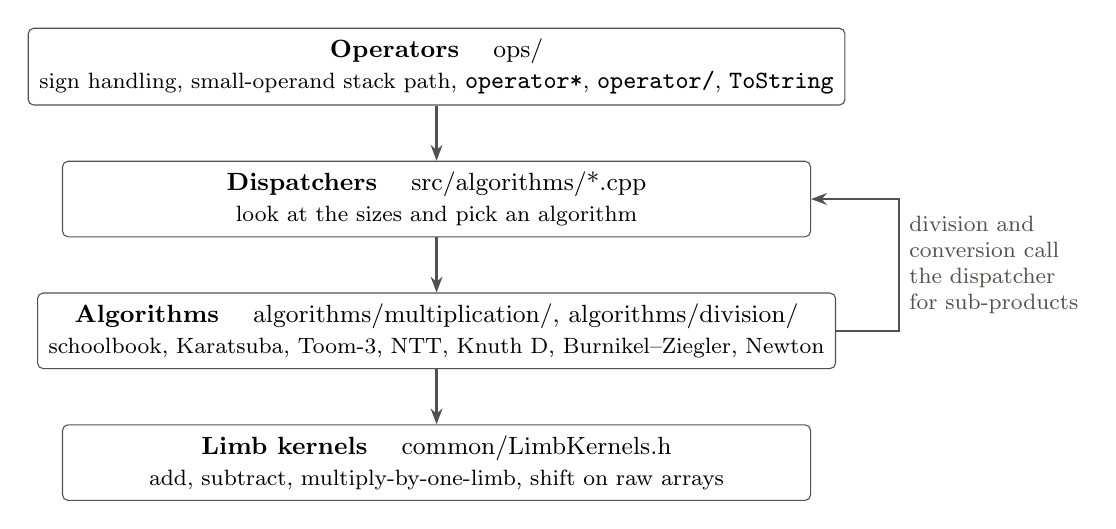
\begin{tikzpicture}[node distance=7mm]
  \node[box,minimum width=95mm] (ops) {\textbf{Operators} \quad \file{ops/}\\ \footnotesize sign handling, small-operand stack path, \code{operator*}, \code{operator/}, \code{ToString}};
  \node[box,minimum width=95mm,below=of ops] (disp) {\textbf{Dispatchers} \quad \file{src/algorithms/*.cpp}\\ \footnotesize look at the sizes and pick an algorithm};
  \node[box,minimum width=95mm,below=of disp] (alg) {\textbf{Algorithms} \quad \file{algorithms/multiplication/}, \file{algorithms/division/}\\ \footnotesize schoolbook, Karatsuba, Toom-3, NTT, Knuth D, Burnikel--Ziegler, Newton};
  \node[box,minimum width=95mm,below=of alg] (ker) {\textbf{Limb kernels} \quad \file{common/LimbKernels.h}\\ \footnotesize add, subtract, multiply-by-one-limb, shift on raw arrays};
  \draw[arr] (ops) -- (disp);
  \draw[arr] (disp) -- (alg);
  \draw[arr] (alg) -- (ker);
  \draw[arr] (alg.east) -- ++(0.8,0) |- node[pos=0.25,right,lbl,align=left]{division and\\conversion call\\the dispatcher\\for sub-products} (disp.east);
\end{tikzpicture}
\caption{Layers of the library. The upward arrow matters: a division step or a decimal
conversion calls the multiplication dispatcher for its sub-products, so each sub-product
gets the best algorithm for its own size.}
\label{fig:layers}
\end{figure}

Arithmetic operators borrow read-only limb ranges through \code{BigInteger::Limbs()}.
A view holds an address and a length. It can cover inline limbs, heap-backed limbs,
or a slice of either while the original storage stays valid. Kernels keep their
writable output and workspace separate. The upward arrow in \cref{fig:layers} lets
the dispatcher choose the method for each sub-product.

\chapter{Building blocks: add, subtract, multiply by one limb}
\label{ch:basics}

Every big algorithm in this library eventually does the same few things over and over:
add two arrays of limbs, subtract one from another, and add a multiple of one array to
another. These operations are called \emph{kernels}. They live in
\file{include/biginteger/common/LimbKernels.h}. This chapter shows how they work and
why the way they are written matters so much.

\section{Addition with carries}

Adding big numbers is grade-school addition. Add the lowest digits, write down the
result, carry one if it overflowed, move left.

\begin{example}[: the same idea in base 10 and base $2^{64}$]
Base 10, $478 + 256$:
\[
\begin{array}{r@{\quad}l}
8 + 6 = 14 & \text{write } 4, \text{ carry } 1\\
7 + 5 + 1 = 13 & \text{write } 3, \text{ carry } 1\\
4 + 2 + 1 = 7 & \text{write } 7
\end{array}
\qquad\Rightarrow\qquad 734
\]
Base $2^{64}$, adding $[\,2^{64}-1,\ 1\,]$ and $[\,1\,]$ (that is, $(2^{64}+2^{64}-1) + 1$):
\[
\begin{array}{r@{\quad}l}
(2^{64}-1) + 1 = 2^{64} & \text{write } 0, \text{ carry } 1\\
1 + 0 + 1 = 2 & \text{write } 2
\end{array}
\qquad\Rightarrow\qquad [\,0,\ 2\,] = 2 \cdot 2^{64}.
\]
\end{example}

A carry is never more than 1, because the largest possible sum,
$(B-1) + (B-1) + 1 = 2B - 1$, is less than $2B$. Subtraction works the same way with a
\emph{borrow} of 0 or 1.

\section{Multiply an array by one limb}

The workhorse of multiplication and division is ``add $b$ times the array $a$ into the
array $r$'', written \code{AddMul1(r, a, n, b)}. Each step multiplies one limb $a_j$ by
$b$, which gives a two-limb (128-bit) product: a low half and a high half. The low half
goes into position $j$; the high half spills into position $j+1$.

\begin{example}[: $987 \times 6$, digit by digit]
Little-endian digits of 987 are $[7, 8, 9]$. Multiply each by 6:
\[
7\cdot 6 = 42,\qquad 8 \cdot 6 = 48,\qquad 9 \cdot 6 = 54 .
\]
Each product has a low digit (2, 8, 4) and a high digit (4, 4, 5). Position $k$ of the
answer is low digit $k$ plus high digit $k-1$ plus any carry:
\[
\begin{array}{c|cccc}
\text{position} & 0 & 1 & 2 & 3\\ \hline
\text{low of } p_k & 2 & 8 & 4 & \\
\text{high of } p_{k-1} & 0 & 4 & 4 & 5\\
\text{carry in} & 0 & 0 & 1 & 0\\ \hline
\text{digit} & 2 & 2 & 9 & 5
\end{array}
\]
Result $[2,2,9,5] = 5922 = 987 \times 6$. In the library the ``digits'' are 64-bit limbs
and the products are 128-bit, but the bookkeeping is identical.
\end{example}

\section{Why the way you write the loop matters}
\label{sec:flagchain}

The obvious C++ for \code{AddMul1} is

\begin{lstlisting}
unsigned __int128 p = (unsigned __int128)a[j] * b + r[j] + carry;
r[j]  = (uint64_t)p;          // low 64 bits
carry = (uint64_t)(p >> 64);  // high 64 bits feed the next limb
\end{lstlisting}

It is correct, and it was in the library for years. The trouble is the
\code{carry} variable. It holds a whole limb, and the next step cannot begin adding until
it is known. Every step waits for the previous step's 128-bit arithmetic to finish. A
modern processor can start a new multiplication every cycle, but this loop forces it to
work one limb at a time, at 2.5--3.3 cycles per limb.

The kernels in \file{LimbKernels.h} split the work into \textbf{two separate carry
chains}, as in the worked example above:

\begin{enumerate}
  \item \textbf{Chain A} forms the product row: $t_k = \text{low}(p_k) + \text{high}(p_{k-1})$,
        with a one-bit carry.
  \item \textbf{Chain B} adds that row into the result: $r_k \mathrel{+}= t_k$, with its own
        one-bit carry.
\end{enumerate}

Neither chain waits on a full 128-bit value. Both carries are single bits, and the code is
written in straight-line blocks of four limbs with the compiler's carry builtins
(\code{\_\_builtin\_addcll}), so the carry bit stays in the processor's flags register from
one limb to the next. On ARM this compiles to a run of \code{adcs} (add with carry)
instructions, the same instructions a hand-written assembly routine would use.

\begin{figure}[ht]
\centering
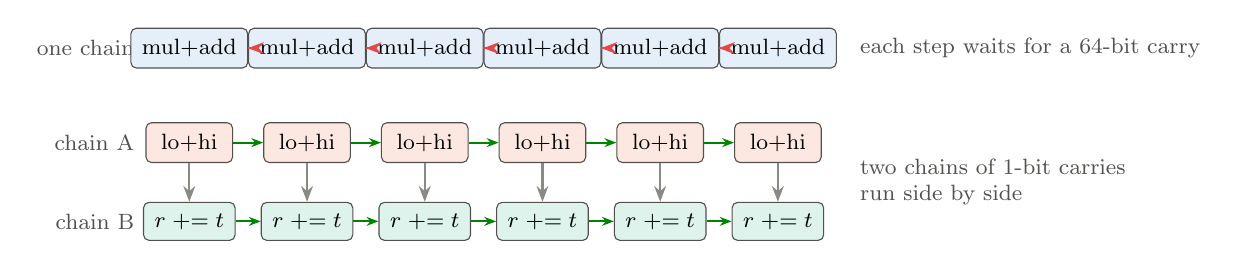
\begin{tikzpicture}[x=1.15cm,y=1cm]
  \node[lbl,anchor=east] at (-0.5,1.6) {one chain};
  \foreach \k in {0,...,5} {
    \node[box,fill=sBlue!12,minimum width=11mm] (o\k) at (\k*1.3,1.6) {\footnotesize mul+add};
  }
  \foreach \k [evaluate=\k as \n using int(\k+1)] in {0,...,4} \draw[arr,sRed] (o\k) -- (o\n);
  \node[lbl,anchor=west] at (7.3,1.6) {each step waits for a 64-bit carry};
  \node[lbl,anchor=east] at (-0.5,0.4) {chain A};
  \node[lbl,anchor=east] at (-0.5,-0.6) {chain B};
  \foreach \k in {0,...,5} {
    \node[box,fill=sOrange!15,minimum width=11mm] (a\k) at (\k*1.3,0.4) {\footnotesize lo+hi};
    \node[box,fill=sAqua!15,minimum width=11mm] (b\k) at (\k*1.3,-0.6) {\footnotesize $r \mathrel{+}= t$};
    \draw[arr,muted] (a\k) -- (b\k);
  }
  \foreach \k [evaluate=\k as \n using int(\k+1)] in {0,...,4} {
    \draw[-{Stealth[length=1.5mm]},sGreen,thick] (a\k) -- (a\n);
    \draw[-{Stealth[length=1.5mm]},sGreen,thick] (b\k) -- (b\n);
  }
  \node[lbl,anchor=west,align=left] at (7.3,-0.1) {two chains of 1-bit carries\\run side by side};
\end{tikzpicture}
\caption{Dependency chains in \code{AddMul1}. Red: the old loop passes a full limb from
step to step. Green: the new kernel passes only carry bits, along two independent
chains that the processor overlaps.}
\end{figure}

\begin{perfnote}
Cycles per limb on an M1 core:
\begin{center}
\begin{tabular}{lccc}
\toprule
kernel & old loop & GMP (hand assembly) & new kernel \\
\midrule
\code{addmul\_1} & 2.5--3.3 & 1.3--1.8 & 1.64--1.76 \\
\code{add\_n} & 2.2--3.3 & 0.65--0.9 & 1.1--1.7 \\
\code{submul\_1} (division) & 2.9--4.0 & 1.3--1.8 & 1.6--1.8 \\
\bottomrule
\end{tabular}
\end{center}
Schoolbook multiplication became 1.5--1.8 times faster, with no assembly language
anywhere in the library. Earlier the gap to GMP had been blamed on ``portable C++ cannot
match assembly''. It turned out the gap was mostly how the loop was written.
\end{perfnote}

\begin{pitfall}
Before this change, an attempt to speed up schoolbook by processing two rows at once
(``2-row unrolling'') measured no gain at all. It kept the same limb-valued carry, so
it kept the same bottleneck. Speed came from changing the \emph{dependency structure}, not
from doing more work per loop iteration.
\end{pitfall}

\section{The kernel set}

\begin{center}
\small
\begin{tabularx}{\textwidth}{lX}
\toprule
kernel & what it computes \\
\midrule
\code{AddN}, \code{SubN} & $r = a \pm b$, arrays of equal length, returns carry / borrow \\
\code{Mul1} & $r = a \cdot b$ for a single limb $b$ \\
\code{AddMul1} & $r \mathrel{+}= a \cdot b$ (one row of schoolbook multiplication) \\
\code{SubMul1} & $r \mathrel{-}= a \cdot b$ (one step of long division) \\
\code{MulBasecase} & schoolbook product: one \code{Mul1} row then \code{AddMul1} rows \\
\code{SqrBasecase} & schoolbook square (\cref{sec:square}) \\
\code{Lshift}, \code{Rshift} & shift an array left or right by 0--63 bits \\
\bottomrule
\end{tabularx}
\end{center}

These kernels are used only with true 64-bit limbs. The legacy layout
(\code{-DBIGMATH\_LIMB\_64=0}) keeps its own simpler loops.

\newpage
\section{Parallel addition and subtraction}
\label{sec:paralleladdsub}

A carry or borrow can cross the entire number. BigMath splits the magnitude into
contiguous blocks and computes each block with an incoming flag of zero. It then
uses the provisional results to determine which blocks need correction. The sign
handling still happens in the operator layer, so adding opposite signs can use
the magnitude subtraction kernel.

\begin{enumerate}
  \item Each block runs the ordinary limb kernel and saves its outgoing carry
        or borrow. For addition it finds the run of all-ones limbs at the low end
        of its provisional result. For subtraction it finds the run of zeros.
  \item A short serial pass visits blocks from low to high. Each block passes
        along its own outgoing flag, or an incoming flag if the run covers the
        entire block. This determines the incoming flag for every block.
  \item A block receiving a carry turns its run of all-ones limbs into zeros
        and increments the next limb, if present. A block receiving a borrow
        turns its zeros into all-ones limbs and decrements the next limb. If at
        least two corrections have runs of 16\,384 limbs or more, the pool
        splits the fixup work again. Otherwise the caller applies the corrections.
\end{enumerate}

\begin{example}
Split $9999 + 1$ into two-digit blocks. The low block computes $99+1$, writes
$00$ and sends a carry. The high block provisionally writes $99$. Its incoming
carry turns both digits to zero and continues beyond the high block, giving $10000$.
\end{example}

In a threaded 64-bit build, the dispatcher considers this path for equal-length
magnitudes above the stack-buffer path, with at least 2\,048 limbs per block.
Addition and subtraction each have a warm and a parked cutoff, measured in
limbs per operand. The checked-in profiles inherit zero for all four cutoffs,
so their magnitude addition and subtraction run serially. The kernel is in
\file{include/biginteger/algorithms/ParallelAddSub.h}.

\subsection*{Choosing the cutoffs}

The tuner requires a speedup of at least $1.05\times$ on both random operands and
full carry or borrow chains at two adjacent sizes and every larger sampled size.
The workflow selects the highest cutoff supported by all three surveys. The hosted
survey selected zero on all five release targets. A native M1 Max survey gave
these machine-specific cutoffs, in limbs per operand.

\begin{center}
\small
\begin{tabular}{lrr}
\toprule
Magnitude operation & Warm & Parked \\
\midrule
Addition    & 24\,576 & 98\,304 \\
Subtraction & 16\,384 & 1\,048\,576 \\
\bottomrule
\end{tabular}
\end{center}

In the native holdout on random equal-length inputs, the public operators' geometric
mean speedups for addition and subtraction were $1.77\times$ and $2.24\times$ in
bursts and $1.54\times$ and $1.09\times$ with parked workers. The parked borrow-chain
group averaged $0.97\times$. See \file{BENCHMARK.md}, \file{docs/PLATFORM\_TUNING.md}
and the build macros in \cref{app:ref}.

\newpage
\section{Comparison and shifts}

For numeric ordering, \code{CompareTo} checks the signs first and reverses
the magnitude order when both values are negative. The relational operators
\code{>}, \code{>=}, \code{<}, and \code{<=} use this same result.

The raw \code{Compare} routine treats high zero limbs as padding. If the
stored lengths differ, any nonzero limb in the longer operand's excess
range decides the comparison. Otherwise, compare the common width. Check
its two highest limbs individually, then scan the remaining limbs in
blocks of 16 when the range is long enough. In each block, XOR corresponding
limbs and OR the differences together. A zero result skips the entire block.
In the first differing block, compare whole limbs from most to least
significant. The same block scan can recognize shared storage, and raw
comparison with a scalar can skip blocks of high zeros.

\begin{example}
Suppose the highest difference is $0\mathrm{x}0100$ on the left and
$0\mathrm{x}00\mathrm{ff}$ on the right, and a lower limb is smaller on
the left. The left value is larger because the highest differing limb
decides. Comparing the first unequal bytes in memory would give a
different result on a little-endian machine.
\end{example}

The worst case remains $O(n)$ time and $O(1)$ extra space.
In the M1 Max benchmark, an ordered comparison of 4,096 limbs with a
low-limb mismatch took about 0.45\,\textmu s, down from
1.30\,\textmu s. Comparisons settled by different lengths took
about $0.7$\,ns longer. See \file{BENCHMARK.md} for the cases and commands.

For \code{a == b}, comparing an object with itself takes constant time. For distinct
objects, the operator checks the signs, stored lengths and outermost limbs. If lengths
differ and the longer value has a high zero limb, it compares the magnitudes to account
for padding. For long values of the same width, it checks the lowest eight limbs as a
block, then compares eight limbs at a time from the high end. This catches small
low-order changes immediately and still exits early for differences near the top.
Equal copies require an exact scan of all $n$ limbs, taking $O(n)$ time and $O(1)$
extra space. The \code{!=} operator uses the same equality check.

The public shift operators count whole limbs. \code{a << k} multiplies
by $B^k$, and \code{a >> k} drops the lowest $k$ limbs while preserving
the sign of a nonzero result. Internally, a shift by $s$ bits splits into
$\floor{s/64}$ whole limbs and $s\bmod 64$ bits in the default radix.
Division uses those bit shifts to normalize the divisor
(\cref{sec:normalize}).

The shared limb utilities use \code{DataT} for stored limb values and
\code{SizeT} for the library's limb counts. Container offsets use
\code{std::size\_t}. Division shares a leading-zero count for
normalization and a trimmed limb count for padded operands.

\chapter{Multiplication I: schoolbook, Karatsuba, and Toom}
\label{ch:mul}

Multiplication is the operation that matters most. Division, square roots, decimal
conversion, and powers are all built out of multiplications, so their speed follows
multiplication's speed. The default dispatcher starts with schoolbook, then uses
Karatsuba (which can split three ways), then switches to the NTT.

\begin{center}
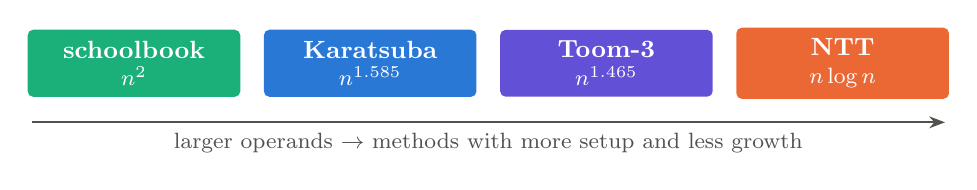
\begin{tikzpicture}
  \foreach \x/\c/\t/\s in {0/sAqua/schoolbook/{$n^2$},1/sBlue/Karatsuba/{$n^{1.585}$},2/sViolet/Toom-3/{$n^{1.465}$},3/sOrange/NTT/{$n\log n$}} {
    \node[algo,fill=\c,minimum width=27mm] at (\x*3,0) {\t\\[-1pt]\footnotesize\s};
  }
  \draw[arr] (-1.3,-0.75) -- node[below,lbl]{larger operands $\rightarrow$ methods with more setup and less growth} (10.3,-0.75);
\end{tikzpicture}
\end{center}

This chapter explains the direct multiplication methods, including the
experimental higher-degree Toom splits. \Cref{ch:ntt,ch:fermat} cover transform methods.
\Cref{ch:muldispatch} explains how the library chooses.

\section{Schoolbook multiplication}
\label{sec:schoolbook}

This is long multiplication as taught in school: multiply the first number by each limb
of the second, shift each partial product one limb further left, and add them all up.

\begin{example}[: $123 \times 45$ in base 10]
\[
\begin{array}{c@{\,}c@{\,}c@{\,}c@{\,}c@{\qquad}l}
 & & 1 & 2 & 3 & \\
\times & & & 4 & 5 & \\ \cline{1-5}
 & & 6 & 1 & 5 & \text{row 1: } 123 \times 5 \\
 & 4 & 9 & 2 & & \text{row 2: } 123 \times 4, \text{ shifted one place} \\ \cline{1-5}
 & 5 & 5 & 3 & 5 & \text{sum of the rows}
\end{array}
\]
Each row is one call of the \code{AddMul1} kernel from \cref{ch:basics}: ``add 123 times
one digit into the running total, at the right offset''.
\end{example}

\begin{figure}[ht]
\centering
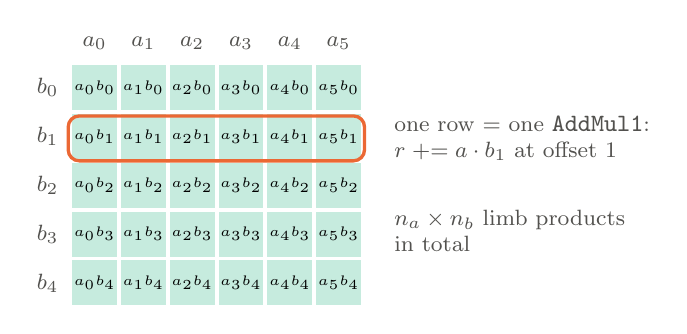
\begin{tikzpicture}[scale=0.62]
  \foreach \i in {0,...,5} \foreach \j in {0,...,4} {
    \fill[sAqua!25] (\i,-\j) rectangle +(0.92,-0.92);
    \node[font=\tiny] at (\i+0.46,-\j-0.46) {$a_{\i}b_{\j}$};
  }
  \foreach \i in {0,...,5} \node[lbl] at (\i+0.46,0.45) {$a_\i$};
  \foreach \j in {0,...,4} \node[lbl] at (-0.5,-\j-0.46) {$b_\j$};
  \draw[sOrange,very thick,rounded corners] (-0.08,-1.04) rectangle (5.99,-1.96);
  \node[lbl,anchor=west,align=left] at (6.4,-1.5) {one row = one \code{AddMul1}:\\$r \mathrel{+}= a \cdot b_1$ at offset 1};
  \node[lbl,anchor=west,align=left] at (6.4,-3.4) {$n_a \times n_b$ limb products\\in total};
\end{tikzpicture}
\caption{Schoolbook multiplication computes every product $a_i b_j$ once. With $n$-limb
operands that is $n^2$ limb multiplications.}
\end{figure}

Schoolbook needs $n_a \times n_b$ limb products. For two 1000-limb numbers that is a
million. The 64-bit Classic path calls \code{MulBasecase} on the original limb ranges.
It writes the first row to the product buffer with \code{Mul1} and accumulates the
rest with \code{AddMul1}. The inner loop scans the longer operand. A one-limb
operand uses the scalar path.

\section{Squaring: half the work}
\label{sec:square}

When both operands are the same number, half of the products are duplicates:
$a_i a_j$ and $a_j a_i$ are equal. A square therefore needs only the products above the
diagonal, doubled, plus the diagonal terms $a_i^2$.

\begin{figure}[ht]
\centering
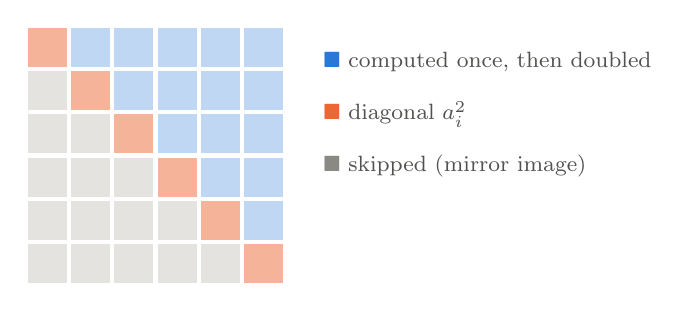
\begin{tikzpicture}[scale=0.55]
  \foreach \i in {0,...,5} \foreach \j in {0,...,5} {
    \ifnum\i>\j \fill[sBlue!30] (\i,-\j) rectangle +(0.9,-0.9);
    \else\ifnum\i=\j \fill[sOrange!50] (\i,-\j) rectangle +(0.9,-0.9);
    \else \fill[rule] (\i,-\j) rectangle +(0.9,-0.9); \fi\fi
  }
  \node[lbl,anchor=west,align=left] at (6.6,-0.8) {\textcolor{sBlue}{$\blacksquare$} computed once, then doubled};
  \node[lbl,anchor=west,align=left] at (6.6,-2.0) {\textcolor{sOrange}{$\blacksquare$} diagonal $a_i^2$};
  \node[lbl,anchor=west,align=left] at (6.6,-3.2) {\textcolor{muted}{$\blacksquare$} skipped (mirror image)};
\end{tikzpicture}
\caption{Schoolbook squaring: about $n^2/2$ products instead of $n^2$.}
\end{figure}

\code{SqrBasecase} computes the off-diagonal rows with \code{AddMul1}, then doubles them
(a one-bit left shift) and adds the diagonal in a single pass. Every faster method in this
chapter also has a squaring version that exploits the same symmetry.

\section{Karatsuba: three multiplications instead of four}
\label{sec:karatsuba}

Split each number into a high half and a low half. In base 10 with 4-digit numbers,
$1234 = 12 \cdot 100 + 34$. Then
\[
(a_1 X + a_0)(b_1 X + b_0) = a_1 b_1 X^2 + (a_1 b_0 + a_0 b_1) X + a_0 b_0 .
\]
Done directly, that is four half-size multiplications: $a_1b_1$, $a_1b_0$, $a_0b_1$, $a_0b_0$.
Anatoly Karatsuba noticed in 1960 that the middle term can be had with \emph{one}
multiplication instead of two:
\[
a_1 b_0 + a_0 b_1 = (a_1 + a_0)(b_1 + b_0) - a_1 b_1 - a_0 b_0 .
\]
The two products on the right, $a_1b_1$ and $a_0b_0$, are needed anyway. So three
half-size multiplications are enough, plus a few additions and subtractions, which are
cheap.

\begin{example}[: $1234 \times 5678$ with three multiplications]
Split at $X = 100$: $a_1 = 12$, $a_0 = 34$, $b_1 = 56$, $b_0 = 78$.
\begin{align*}
z_2 &= a_1 b_1 = 12 \times 56 = 672\\
z_0 &= a_0 b_0 = 34 \times 78 = 2652\\
z_1 &= (a_1 + a_0)(b_1 + b_0) - z_2 - z_0 = 46 \times 134 - 672 - 2652 = 6164 - 3324 = 2840
\end{align*}
Put the pieces together:
\[
672 \cdot 10^4 + 2840 \cdot 10^2 + 2652 = 6\,720\,000 + 284\,000 + 2\,652 = 7\,006\,652 .
\]
And indeed $1234 \times 5678 = 7\,006\,652$, using three two-digit multiplications
instead of four.
\end{example}

The trick is applied \emph{recursively}: each of the three half-size products is itself
computed with Karatsuba, until the pieces are small enough that schoolbook is faster.

\begin{figure}[ht]
\centering
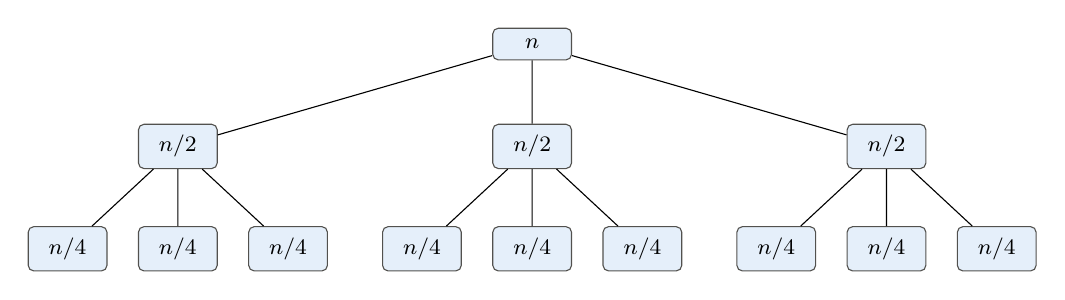
\begin{tikzpicture}[level distance=13mm,
  level 1/.style={sibling distance=45mm},
  level 2/.style={sibling distance=14mm},
  every node/.style={box,fill=sBlue!12,font=\footnotesize,minimum width=10mm}]
  \node {$n$}
    child {node {$n/2$} child {node {$n/4$}} child {node {$n/4$}} child {node {$n/4$}}}
    child {node {$n/2$} child {node {$n/4$}} child {node {$n/4$}} child {node {$n/4$}}}
    child {node {$n/2$} child {node {$n/4$}} child {node {$n/4$}} child {node {$n/4$}}};
\end{tikzpicture}
\caption{Karatsuba's recursion. Each level has three times as many sub-products, each
half as long. Schoolbook would have four times as many at each level.}
\end{figure}

\paragraph{How much does it save?} Halving the size cuts a schoolbook product's cost by 4
but Karatsuba only needs 3 of them. After $k$ levels there are $3^k$ products of size
$n/2^k$, so the total is about $n^{\log_2 3} \approx n^{1.585}$ instead of $n^2$.
\Cref{fig:mulcounts} shows the exact count of limb products for the library's actual
recursion: at 1000 limbs Karatsuba needs about a fifth of schoolbook's products, at 8000
limbs under a tenth.

\begin{figure}[ht]
\centering
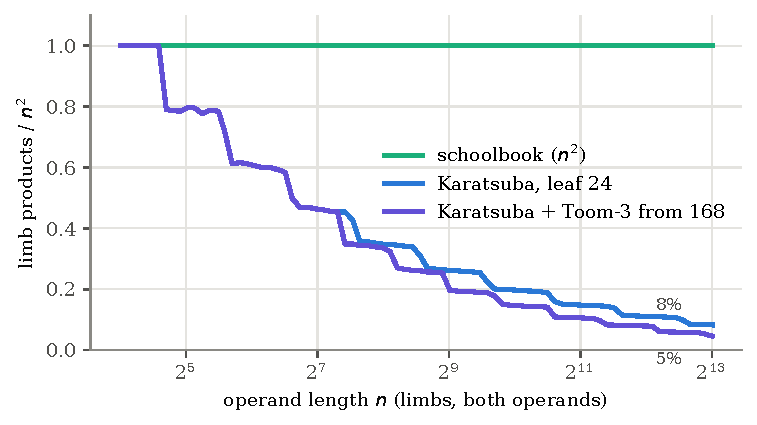
\includegraphics[width=0.8\textwidth]{figures/mul_counts.pdf}
\caption{Limb products needed, as a fraction of schoolbook's $n^2$, for the library's
recursion (leaf at 24 limbs, Toom-3 levels from 168 limbs). Computed exactly by
\file{figures/make\_figures.py}. Fewer products is not the whole story: the extra
additions and memory traffic are why the crossover sizes have to be measured.}
\label{fig:mulcounts}
\end{figure}

\subsection{Where the recursion stops}

Each Karatsuba level costs some additions, subtractions and bookkeeping. For short
pieces that overhead is larger than the multiplication it saves. The recursion therefore
stops at \code{BIGMATH\_KARATSUBA\_THRESHOLD} $= 24$ limbs and hands the piece to the
schoolbook kernel.

This cutoff has moved over time, which shows how measurement-driven it is: 48 limbs in
May 2026, 32 in June after the NTT got faster, and 24 in November after the flag-chain
kernels (\cref{sec:flagchain}) made Karatsuba's own additions cheaper. Cheaper overhead
means one more level of recursion pays off.

\subsection{Unequal sizes: slicing}

What if one number is much longer than the other, say $5000 \times 100$ limbs? Splitting
both ``in half'' makes no sense, because the short one has no high half. When one operand
is at least twice as long as the other, BigMath \emph{slices} the long operand into pieces
as long as the short one, multiplies each piece by the short operand (a balanced product),
and adds the pieces at their offsets.

\begin{figure}[ht]
\centering
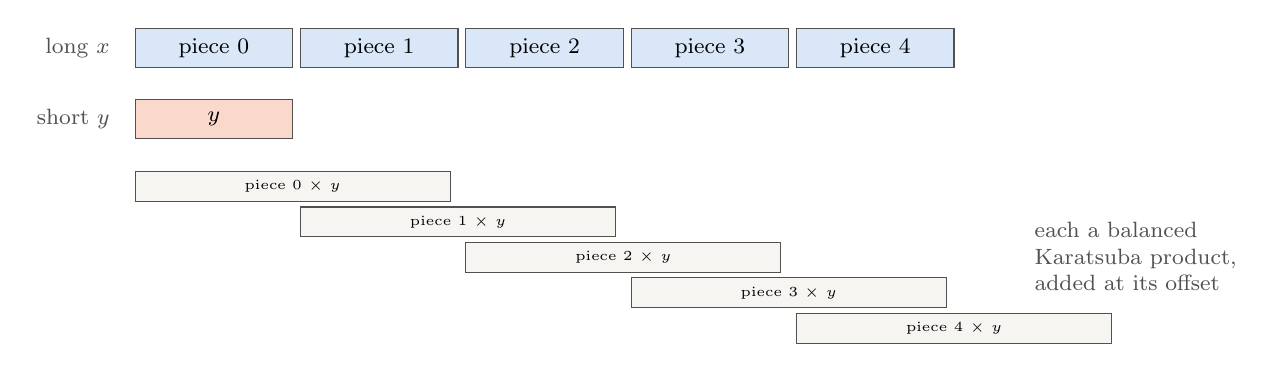
\begin{tikzpicture}[x=1cm,y=1cm]
  \foreach \k in {0,...,4} {
    \fill[sBlue!18,draw=ink2] (\k*2.1,0) rectangle +(2,0.5);
    \node[font=\footnotesize] at (\k*2.1+1,0.25) {piece \k};
  }
  \node[lbl,anchor=east] at (-0.2,0.25) {long $x$};
  \fill[sOrange!25,draw=ink2] (0,-0.9) rectangle +(2,0.5);
  \node[font=\footnotesize] at (1,-0.65) {$y$};
  \node[lbl,anchor=east] at (-0.2,-0.65) {short $y$};
  \foreach \k in {0,...,4} {
    \draw[draw=ink2,fill=paper] (\k*2.1,-1.7-\k*0.45) rectangle +(4,0.38);
    \node[font=\tiny] at (\k*2.1+2,-1.51-\k*0.45) {piece \k\ $\times\ y$};
  }
  \node[lbl,anchor=west,align=left] at (11.3,-2.4) {each a balanced\\Karatsuba product,\\added at its offset};
\end{tikzpicture}
\caption{Slicing an unbalanced product into balanced ones.}
\end{figure}

The cost is the number of pieces times the cost of one balanced product: roughly
$n_{\max} \cdot K(n_{\min}) / n_{\min}$, where $K(m)$ is the cost of an $m \times m$
Karatsuba product. It grows \emph{linearly} with the long operand, at a rate set by the
short one. This is the key to choosing between Karatsuba and the NTT for lopsided shapes
(\cref{sec:arearule}).

\begin{pitfall}
Before slicing, the code just clamped the split point. For very lopsided shapes the
recursion then peeled off only a few limbs per level, ran $n_{\max}/n_{\min}$ levels deep
instead of $\log_2 n$, and its scratch space grew like $n_{\max}^2/n_{\min}$. On shapes the
dispatcher really sent there (for example $1214 \times 65$ limbs) that overflowed the
workspace buffer. Slicing fixed both the speed and the memory bound (about $4 n_{\max}$).
\end{pitfall}

\begin{perfnote}
The recursive multiplier reads operand ranges through pointers and partitions a
workspace sized before recursion starts. Requests of up to 2\,048 scratch limbs
use a stack buffer. Larger requests use heap storage. Inner calls write the
output and middle term directly. An earlier vector-based Karatsuba square lost
to plain multiplication at 128 limbs because of allocation and zero-fill costs.
\end{perfnote}

\section{Toom-3: split in three}
\label{sec:toom}

Karatsuba splits into halves. Why not thirds? Splitting into three parts gives
nine sub-products done naively; Toom-Cook (Andrei Toom 1963, Stephen Cook 1966) gets by
with \emph{five}. The cost becomes $n^{\log_3 5} \approx n^{1.465}$.

\subsection{The polynomial view}

Write each operand as a polynomial in the split point $X$:
\[
a = a_2 X^2 + a_1 X + a_0 \quad\longrightarrow\quad p(x) = a_2 x^2 + a_1 x + a_0 .
\]
Then $a \cdot b$ is the polynomial product $r(x) = p(x)\,q(x)$ evaluated at $x = X$. The
product has degree 4, so it has five unknown coefficients $r_0,\dots,r_4$. A degree-4
polynomial is fixed by its values at any five points. So:

\begin{enumerate}
  \item \textbf{Evaluate} $p$ and $q$ at five points. BigMath uses $0, 1, -1, 2$ and
        ``$\infty$'' (which simply means the top coefficient).
  \item \textbf{Multiply} the values pairwise: five products, each about one third as long
        as the inputs. These are done recursively.
  \item \textbf{Interpolate}: recover $r_0,\dots,r_4$ from the five values.
  \item \textbf{Recompose}: $a b = r_4 X^4 + r_3 X^3 + r_2 X^2 + r_1 X + r_0$, adding the
        overlapping pieces with carries.
\end{enumerate}

\begin{figure}[ht]
\centering
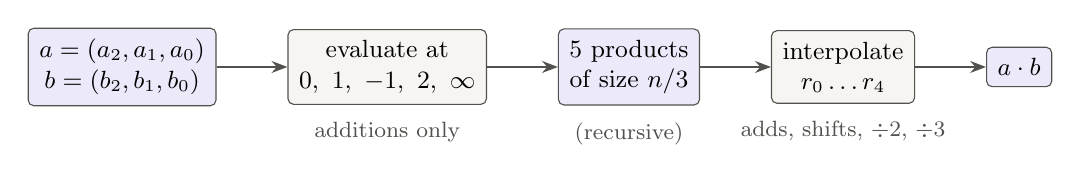
\begin{tikzpicture}[node distance=4mm and 9mm]
  \node[box,fill=sViolet!12] (in) {$a = (a_2, a_1, a_0)$\\$b = (b_2, b_1, b_0)$};
  \node[box,right=of in,fill=paper] (ev) {evaluate at\\$0,\ 1,\ -1,\ 2,\ \infty$};
  \node[box,right=of ev,fill=sViolet!12] (mul) {5 products\\of size $n/3$};
  \node[box,right=of mul,fill=paper] (int) {interpolate\\$r_0 \dots r_4$};
  \node[box,right=of int,fill=sViolet!12] (out) {$a \cdot b$};
  \draw[arr] (in) -- (ev); \draw[arr] (ev) -- (mul); \draw[arr] (mul) -- (int); \draw[arr] (int) -- (out);
  \node[lbl,below=1mm of mul] {(recursive)};
  \node[lbl,below=1mm of ev] {additions only};
  \node[lbl,below=1mm of int] {adds, shifts, $\div 2$, $\div 3$};
\end{tikzpicture}
\caption{Evaluate, multiply, interpolate. Only the middle step multiplies.}
\label{fig:evalinterp}
\end{figure}

\begin{example}[: $123 \times 456$ with Toom-3]
Split at $X = 10$: $p(x) = x^2 + 2x + 3$ and $q(x) = 4x^2 + 5x + 6$.

\textbf{Evaluate} (additions only):
\begin{center}
\begin{tabular}{lccccc}
\toprule
point & $0$ & $1$ & $-1$ & $2$ & $\infty$ \\
\midrule
$p$ & 3 & 6 & 2 & 11 & 1 \\
$q$ & 6 & 15 & 5 & 32 & 4 \\
\midrule
product $v$ & $v_0 = 18$ & $v_1 = 90$ & $v_{-1} = 10$ & $v_2 = 352$ & $v_\infty = 4$ \\
\bottomrule
\end{tabular}
\end{center}

\textbf{Interpolate} with Bodrato's sequence, the one the library uses. Every line is an
addition, a subtraction, or an exact division by 2 or 3:
\begin{align*}
v_2 &\leftarrow (v_2 - v_{-1})/3 = (352 - 10)/3 = 114 && = r_1 + r_2 + 3r_3 + 5r_4\\
v_{-1} &\leftarrow (v_1 - v_{-1})/2 = (90 - 10)/2 = 40 && = r_1 + r_3\\
v_1 &\leftarrow v_1 - v_0 = 90 - 18 = 72 && = r_1 + r_2 + r_3 + r_4\\
v_2 &\leftarrow (v_2 - v_1)/2 = (114 - 72)/2 = 21 && = r_3 + 2 r_4\\
v_1 &\leftarrow v_1 - v_{-1} - v_\infty = 72 - 40 - 4 = 28 && = r_2\\
v_2 &\leftarrow v_2 - 2 v_\infty = 21 - 8 = 13 && = r_3\\
v_{-1} &\leftarrow v_{-1} - v_2 = 40 - 13 = 27 && = r_1
\end{align*}
So $r = (r_4, r_3, r_2, r_1, r_0) = (4, 13, 28, 27, 18)$.

\textbf{Recompose} at $x = 10$: $40000 + 13000 + 2800 + 270 + 18 = 56088$, and
$123 \times 456 = 56088$. Five small products replaced nine.
\end{example}

\begin{another}[: Karatsuba is Toom-2]
The product $(a_1x + a_0)(b_1x + b_0)$ has degree 2. At $0$, $1$ and $\infty$ it
gives Karatsuba's three products $a_0b_0$, $(a_0 + a_1)(b_0 + b_1)$ and $a_1b_1$.
Subtracting $z_0$ and $z_2$ gives the middle coefficient. Toom-$k$ uses $2k-1$
points. More pieces lower the exponent and raise evaluation and interpolation
costs. \Cref{ch:ntt} takes the same idea further.
\end{another}

\subsection{Why the sequence runs on unsigned numbers}

Look at the right-hand column of the interpolation: every intermediate value is a
combination of the $r_i$ with non-negative weights, and the $r_i$ themselves are never
negative (they are sums of products of limbs). So no intermediate value is ever negative,
and the whole interpolation runs on plain unsigned limb arrays with the fast kernels. Only
$v_{-1}$ can be negative, since $p(-1)$ and $q(-1)$ can be; its sign is tracked separately
and folded into the first two steps. The exact division by 3 is a multiplication by the
inverse of 3 modulo $2^{64}$ (\code{0xAAAA\ldots AAB}), which is much cheaper than a real
division.

\subsection{Where Toom-3 is used}

Toom-3 lives \emph{inside} the Karatsuba recursion: at each level, if the shorter operand
has at least \code{BIGMATH\_MUL\_TOOM33\_THRESHOLD} $= 168$ limbs (160 for squares) and both
operands have a non-empty top third, the level splits three ways; otherwise it halves as
usual. Because the choice is made at every level, every sub-product picks the best split
for its own size, including the pieces of sliced unbalanced products and the products
inside division.

Measured on balanced products (microseconds):

\begin{center}
\begin{tabular}{lrrrrrrr}
\toprule
limbs & 160 & 176 & 192 & 224 & 384 & 512 & 768 \\
\midrule
Karatsuba only & 7.38 & 9.20 & 10.21 & 13.40 & 31.60 & 48.76 & 96.44 \\
with Toom-3 & 7.37 & 8.60 & 9.55 & 12.64 & 28.76 & 45.73 & 86.53 \\
\bottomrule
\end{tabular}
\end{center}

A 5--10\% gain. Modest, because balanced products from about 310 limbs go to the NTT when
the thread pool is awake. Toom-3 matters most for cold calls and for the unbalanced pieces
and division sub-products that stay below the NTT.

\begin{practice}
The public multiplication operator reaches the limb-based Toom-3 through
Karatsuba. The optional four-way split has a default cutoff of $10^6$ limbs,
effectively out of reach before the NTT takes over.
\end{practice}

\clearpage
\section{Toom-5: nine products from five pieces}
\label{sec:toomfive}

Take five chunks from each operand, keeping them in order from low to high.
Divide the longer length by five and round up to get the chunk width $k$
in limbs. Missing high chunks are zero. Each chunk's place value is a
power of $X=B^k$.
For example, the first operand is $a_0+a_1X+\cdots+a_4X^4$. Think of
that expression as a recipe. Replace $X$ temporarily by a small number
$x$ and you can mix the five chunks using additions and short integer
multiplications. Mix both inputs with the same $x$, then multiply the
two mixed values.

\begin{figure}[H]
\centering
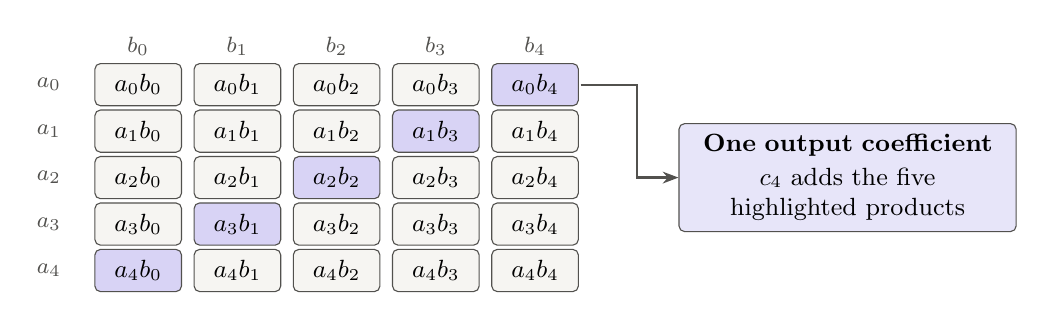
\begin{tikzpicture}[x=1.26cm,y=0.59cm]
  \foreach \i in {0,...,4} {
    \node[lbl] at (\i,0.83) {$b_{\i}$};
    \node[lbl] at (-0.9,-\i) {$a_{\i}$};
    \foreach \j in {0,...,4} {
      \pgfmathtruncatemacro{\degree}{\i+\j}
      \ifnum\degree=4
        \node[box,minimum width=11mm,fill=sViolet!25] at (\j,-\i) {$a_{\i}b_{\j}$};
      \else
        \node[box,minimum width=11mm,fill=paper] at (\j,-\i) {$a_{\i}b_{\j}$};
      \fi
    }
  }
  \node[box,fill=sViolet!15,text width=40mm] (middle) at (7.15,-2)
    {\textbf{One output coefficient}\\[1pt]$c_4$ adds the five\\highlighted products};
  \draw[arr] (4.46,0) -- (5.03,0) |- (middle.west);
\end{tikzpicture}
\caption{Direct multiplication makes 25 chunk products. All entries with
$i+j=4$ contribute to the same power of the chunk base. The whole grid gives
nine coefficients, $c_0$ through $c_8$.}
\end{figure}

Toom-5 recovers those same nine coefficients from nine products of mixed
values. Two come straight from the ends. The low chunks give $c_0$ and
the high chunks give $c_8$, written as the values at $0$ and $\infty$.
Seven other points each supply one equation in the seven middle
coefficients. Solving those equations is called \emph{interpolation}.
The hand example uses integer points. The limb implementation uses
$\pm1/2,\pm1,\pm2$ and $4$, so it can scale the evaluations by powers of two.

\begin{figure}[H]
\centering
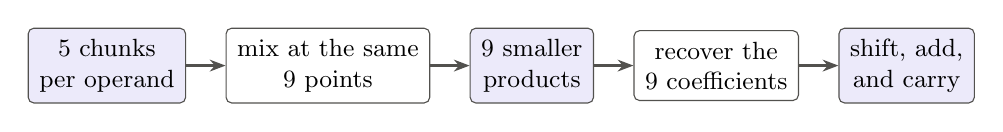
\begin{tikzpicture}[node distance=5mm]
  \node[box,fill=sViolet!12] (input) {5 chunks\\per operand};
  \node[box,right=of input] (mix) {mix at the same\\9 points};
  \node[box,fill=sViolet!12,right=of mix] (mul) {9 smaller\\products};
  \node[box,right=of mul] (solve) {recover the\\9 coefficients};
  \node[box,fill=sViolet!12,right=of solve] (out) {shift, add,\\and carry};
  \draw[arr] (input) -- (mix);
  \draw[arr] (mix) -- (mul);
  \draw[arr] (mul) -- (solve);
  \draw[arr] (solve) -- (out);
\end{tikzpicture}
\caption{Each mixed product replaces work on the original chunks. Interpolation
puts the products back into their original place values.}
\end{figure}

Ideally a five-way recursion grows like $n^{\log_5 9}\approx n^{1.365}$,
versus $n^{\log_3 5}\approx n^{1.465}$ for Toom-3. Evaluation and
interpolation involve many extra passes over the pieces, which matter
at the sizes where the two methods compete.

\newpage
\subsection{Worked example with five decimal chunks}

Multiply $12345$ by $12121$ using one decimal digit per chunk, so $X=10$.
At $x=1$ each mixed value is just the sum of its digits. At $x=-1$ the
second input gives $1-2+1-2+1=-1$. The sign travels with the product.
The final column uses the two high digits.

\begin{center}
\small
\begin{tabular}{lrrrrrrrrr}
\toprule
point $x$ & $0$ & $1$ & $-1$ & $2$ & $-2$ & $3$ & $-3$ & $4$ & $\infty$ \\
\midrule
first input & 5 & 15 & 3 & 57 & 9 & 179 & 47 & 453 & 1 \\
second input & 1 & 7 & $-1$ & 41 & 1 & 151 & 31 & 409 & 1 \\
product $r(x)$ & 5 & 105 & $-3$ & 2337 & 9 & 27029 & 1457 & 185277 & 1 \\
\bottomrule
\end{tabular}
\end{center}

The endpoints give $c_0=5$ and $c_8=1$. Subtract their contributions to get
$h(x)=r(x)-5-x^8$. At $x$ and $-x$ the even powers have the same sign and
the odd powers have opposite signs. Half the sum isolates the even part,
and half the difference isolates the odd part. At $x=1$ these are
$(99-9)/2=45$ and $(99+9)/2=54$. Dividing the even part by $x^2$ and the
odd part by $x$ leaves two short polynomials in $t=x^2$.

\begin{center}
\small
\begin{tabular}{lrrrr}
\toprule
$t=x^2$ & 1 & 4 & 9 & 16 \\
\midrule
$E(t)=c_2+c_4t+c_6t^2$ & 45 & 228 & 853 & $2400$ \\
$O(t)=c_1+c_3t+c_5t^2+c_7t^3$ & 54 & 582 & 4262 & $20334$ \\
\bottomrule
\end{tabular}
\end{center}

Here is one way to solve the equations by hand. The first two slopes of
$E$ are $(228-45)/3=61$ and $(853-228)/5=125$. Their difference divided
by $9-1$ is $8$. Thus
$E(t)=45+61(t-1)+8(t-1)(t-4)=16+21t+8t^2$. This gives $E(16)=2400$.
The extra reading at $x=4$ gives $O(16)=(119736-16\cdot2400)/4=20334$.
Applying the same slope calculation to $O$ gives
\[
O(t)=54+176(t-1)+70(t-1)(t-4)+4(t-1)(t-4)(t-9)
    =14+22t+14t^2+4t^3 .
\]
The limb implementation uses the same slope calculation. It scales its
fractional samples by powers of two so the grid and the polynomial
coefficients are integers. Each division in interpolation is exact.

\begin{center}
\small
\begin{tabular}{lrrrrrrrrr}
\toprule
place, low to high & 0 & 1 & 2 & 3 & 4 & 5 & 6 & 7 & 8 \\
\midrule
raw coefficient & 5 & 14 & 16 & 22 & 21 & 14 & 8 & 4 & 1 \\
carry in & 0 & 0 & 1 & 1 & 2 & 2 & 1 & 0 & 0 \\
digit after carry & 5 & 4 & 7 & 3 & 3 & 6 & 9 & 4 & 1 \\
\bottomrule
\end{tabular}
\end{center}

At place 2, $16+1=17$ writes $7$ and sends a carry of $1$. Read the final
digits from high to low to get $149\,633\,745$.

\begin{practice}
\file{Toom5Multiplication.h} provides a direct call to the limb-based
implementation. It uses Karatsuba below 512 limbs in the longer operand
and for the legacy radix. The automatic dispatcher uses the existing
recursive and NTT paths. See \file{BENCHMARK.md} for the higher Toom sweep.
\end{practice}

\newpage
\section{Toom-6.5 and Toom-8.5: unequal splits}
\label{sec:toomhalf}

In the half-step variants, one operand gets an extra chunk slot. Toom-6.5
uses seven slots for the longer operand and six for the shorter.
Toom-8.5 uses nine and eight. Both operands use the same chunk width.
When the extra high slot lies beyond the end of an operand, it contributes
zero. For example, a $700\times600$-limb Toom-6.5 product uses 100 limbs
per slot. Each input fits its row exactly.

\begin{figure}[H]
\centering
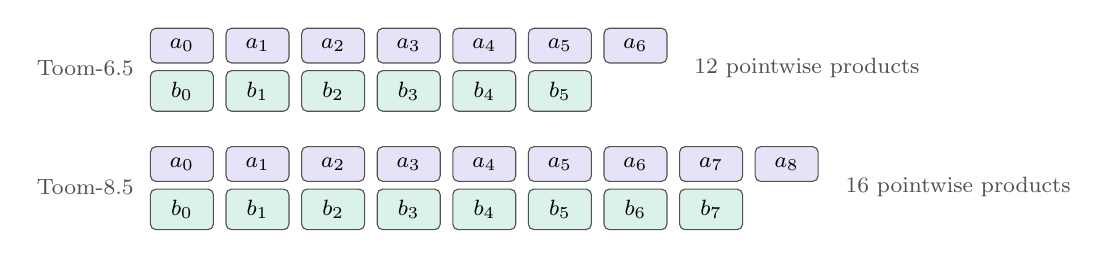
\begin{tikzpicture}[x=0.96cm,y=0.64cm]
  \node[lbl,anchor=east] at (-0.51,0) {Toom-6.5};
  \node[lbl,anchor=east] at (-0.51,-2.35) {Toom-8.5};
  \foreach \i in {0,...,8} {
    \ifnum\i<7
      \node[box,fill=sViolet!16,minimum width=8mm] at (\i,0.45) {\footnotesize $a_{\i}$};
    \fi
    \ifnum\i<6
      \node[box,fill=sAqua!16,minimum width=8mm] at (\i,-0.45) {\footnotesize $b_{\i}$};
    \fi
    \node[box,fill=sViolet!16,minimum width=8mm] at (\i,-1.9) {\footnotesize $a_{\i}$};
    \ifnum\i<8
      \node[box,fill=sAqua!16,minimum width=8mm] at (\i,-2.8) {\footnotesize $b_{\i}$};
    \fi
  }
  \node[lbl,anchor=west] at (6.65,0) {12 pointwise products};
  \node[lbl,anchor=west] at (8.65,-2.35) {16 pointwise products};
\end{tikzpicture}
\caption{The extra slot makes the product degree odd. Two products come
from the ends of the input rows. The remaining products come in pairs
evaluated at a positive point and its negative.}
\end{figure}

For seven by six slots, the two input recipes have degrees six and five,
so their product has degree eleven. Twelve readings determine its
coefficients. Two are the endpoints. The other ten come from
$\pm1/4,\pm1/2,\pm1,\pm2,\pm4$. Adding paired results isolates the even
powers and subtracting them isolates the odd powers. After removing the
endpoints, five even and five odd coefficients are left.

With nine by eight slots the degrees are eight and seven, so there are
sixteen readings. The extra pairs are $\pm1/8$ and $\pm8$. Squaring the
positive points gives a grid whose neighboring values differ by a factor
of four. The code scales it to $1,4,16,\ldots$ and uses the divided
differences from the Toom-5 example to recover the coefficients. Shifts
handle the powers of two. Multiplication by an inverse modulo the limb
base handles each remaining odd divisor exactly.

BigMath's two half-step kernels share the buffer and interpolation code
with limb-based Toom-5. Each forces one outer split, then uses the existing
Karatsuba and Toom-3 recursion for its smaller products. The design uses
the paired powers-of-two idea described in the
\href{https://gmplib.org/manual/Higher-degree-Toom_0027n_0027half}{GNU MP manual}.

\chapter{Multiplication II: the number-theoretic transform}
\label{ch:ntt}

For large numbers BigMath multiplies with a \emph{number-theoretic transform} (NTT), a
version of the fast Fourier transform (FFT) that works with whole numbers modulo a prime
instead of floating-point complex numbers. Its cost grows like $n \log n$, so it beats
every method of \cref{ch:mul} once the numbers are large enough. This chapter builds it up
in steps: first what has to be computed, then why a transform helps, then the tricks that
make BigMath's implementation fast.

\section{Multiplication is a convolution}

Treat each number as a list of digits. When you multiply, digit position $k$ of the
answer (before carrying) collects every product $a_i b_j$ with $i + j = k$:
\[
c_k = \sum_{i + j = k} a_i\, b_j .
\]
This sum-over-diagonals is called a \emph{convolution}. Carrying comes afterwards.

\begin{example}[: $12 \times 34$ as a convolution]
Little-endian digits: $a = (2, 1)$, $b = (4, 3)$.
\begin{align*}
c_0 &= a_0 b_0 = 8\\
c_1 &= a_0 b_1 + a_1 b_0 = 6 + 4 = 10\\
c_2 &= a_1 b_1 = 3
\end{align*}
Now carry: $c_1 = 10$ becomes digit 0 with a carry of 1 into $c_2$, giving digits
$(8, 0, 4)$, that is $408 = 12 \times 34$.
\end{example}

Computing the convolution directly is schoolbook multiplication again: $n^2$ products.
The FFT idea is to compute it a completely different way.

\section{Why a transform helps}

\Cref{sec:toom} showed the recipe ``evaluate at some points, multiply the values
pointwise, interpolate''. A product with $N$ coefficients needs $N$ points. Pointwise
multiplication then costs only $N$ multiplications. The problem is the evaluation and
interpolation: at arbitrary points they cost about $N^2$ each, which gains nothing.

The FFT fixes this by choosing very special points: the $N$-th \emph{roots of unity}, the
$N$ numbers $\omega^0, \omega^1, \dots, \omega^{N-1}$ where $\omega^N = 1$. Their powers
repeat in a pattern that lets an evaluation of size $N$ be split into two evaluations of
size $N/2$, which split again, and so on. That divide-and-conquer brings evaluation down
to about $N \log_2 N$ operations.

\begin{figure}[ht]
\centering
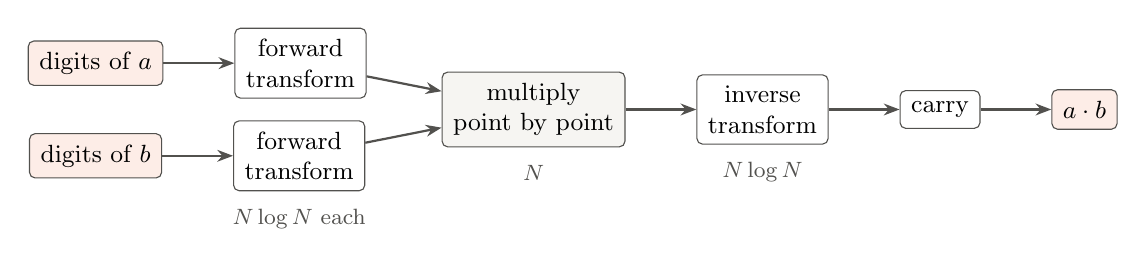
\begin{tikzpicture}[node distance=6mm and 9mm]
  \node[box,fill=sOrange!12] (a) {digits of $a$};
  \node[box,fill=sOrange!12,below=of a] (b) {digits of $b$};
  \node[box,right=of a] (fa) {forward\\transform};
  \node[box,right=of b] (fb) {forward\\transform};
  \node[box,fill=paper,right=18mm of $(fa)!0.5!(fb)$] (pw) {multiply\\point by point};
  \node[box,right=of pw] (inv) {inverse\\transform};
  \node[box,right=of inv] (car) {carry};
  \node[box,fill=sOrange!12,right=of car] (out) {$a\cdot b$};
  \draw[arr] (a) -- (fa); \draw[arr] (b) -- (fb);
  \draw[arr] (fa) -- (pw); \draw[arr] (fb) -- (pw);
  \draw[arr] (pw) -- (inv); \draw[arr] (inv) -- (car); \draw[arr] (car) -- (out);
  \node[lbl,below=1mm of inv] {$N\log N$};
  \node[lbl,below=1mm of pw] {$N$};
  \node[lbl,below=1mm of fb] {$N\log N$ each};
\end{tikzpicture}
\caption{Transform-based multiplication: three transforms, one cheap pointwise pass, one
carry pass.}
\end{figure}

\subsection{Why modulo a prime?}

The textbook FFT uses complex numbers such as $e^{2\pi i/N}$, computed in floating point.
Rounding errors then make it hard to guarantee exact integer results for very large
inputs. In arithmetic modulo a suitable prime $P$ there are also numbers with
$\omega^N = 1$, and every calculation is exact. The transform computes each $c_k$ modulo
$P$; if $P$ is larger than any possible $c_k$, that \emph{is} $c_k$.

\begin{example}[: a complete NTT by hand, modulo 17]
Multiply $12 \times 34$ again, with $N = 4$ points modulo $P = 17$. The number
$\omega = 4$ works as a 4th root of unity: $4^2 = 16 \equiv -1$ and $4^4 \equiv 1 \pmod{17}$.
Its powers are $\omega^0 = 1,\ \omega^1 = 4,\ \omega^2 = 16,\ \omega^3 = 13$.

\textbf{Forward transform}: $A_k = \sum_j a_j\, \omega^{jk} \bmod 17$, with $a = (2,1,0,0)$
and $b = (4,3,0,0)$ padded to length 4:
\begin{center}
\begin{tabular}{lcccc}
\toprule
$k$ & 0 & 1 & 2 & 3 \\
\midrule
$A_k$ & $2+1 = 3$ & $2+4 = 6$ & $2+16 \equiv 1$ & $2+13 \equiv 15$ \\
$B_k$ & $4+3 = 7$ & $4+12 = 16$ & $4+48 \equiv 1$ & $4+39 \equiv 9$ \\
$C_k = A_k B_k$ & $21 \equiv 4$ & $96 \equiv 11$ & $1$ & $135 \equiv 16$ \\
\bottomrule
\end{tabular}
\end{center}

\textbf{Inverse transform}: $c_j = N^{-1} \sum_k C_k\, \omega^{-jk}$. Here $N^{-1} = 4^{-1} = 13$
(since $4 \cdot 13 = 52 \equiv 1$) and the inverse powers are $\omega^{-1} = 13$,
$\omega^{-2} = 16$, $\omega^{-3} = 4$:
\begin{align*}
c_0 &= 13\,(4 + 11 + 1 + 16) = 13 \cdot 32 \equiv 8\\
c_1 &= 13\,(4 + 11\cdot 13 + 1 \cdot 16 + 16 \cdot 4) = 13 \cdot 227 \equiv 10\\
c_2 &= 13\,(4 + 11 \cdot 16 + 1 + 16 \cdot 16) = 13 \cdot 437 \equiv 3\\
c_3 &= 13\,(4 + 11 \cdot 4 + 1 \cdot 16 + 16 \cdot 13) = 13 \cdot 272 \equiv 0
\end{align*}
The result $(8, 10, 3, 0)$ is exactly the convolution from the previous example. Carrying
gives 408.
\end{example}

\subsection{Wrap-around: the transform length must be long enough}

A length-$N$ transform computes the convolution \emph{cyclically}: coefficients past
position $N-1$ wrap around and are added to the start. In the language of polynomials it
computes the product modulo $x^N - 1$. That is why the transform must be at least as long
as the product: with $N = 2$ above, $c_2 = 3$ would have landed on top of $c_0$.

\begin{another}[: wrap-around is not always a bug]
With $N = 2$ the transform gives $(c_0 + c_2,\ c_1) = (11, 10)$, which reads as
$11 + 10 \cdot 10 = 111$. That is not $408$, but it \emph{is} $408$ modulo $10^2 - 1 = 99$
($408 = 4 \cdot 99 + 12$ and $111 = 99 + 12$). In general a cyclic transform of length $L$
computes a product modulo $B^L - 1$ at half the price of the full product. Newton division
uses exactly this (\cref{sec:wrap}): when only the low part of a product is needed, a
wrapped product is enough.
\end{another}

\section{The butterfly: how the transform is fast}

The forward transform of length $N$ splits into two transforms of length $N/2$, joined by
$N/2$ \emph{butterflies}. A butterfly takes two values $u, v$ and a twiddle factor $w$
(a power of $\omega$) and produces $u + v$ and $(u - v)\,w$. After $\log_2 N$ layers of
butterflies the transform is done.

\begin{figure}[ht]
\centering
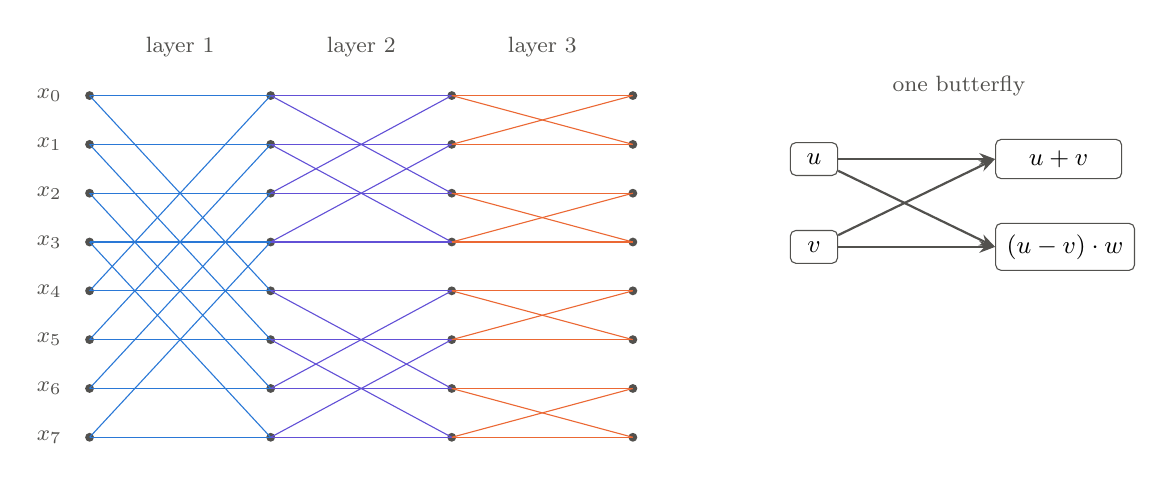
\begin{tikzpicture}[x=2.3cm,y=0.62cm]
  \foreach \s in {0,1,2,3} \foreach \i in {0,...,7} \fill[ink2] (\s,-\i) circle (1.6pt);
  \foreach \i in {0,...,7} \node[lbl,anchor=east] at (-0.1,-\i) {$x_\i$};
  % stage 1: span 4
  \foreach \i in {0,...,3} {
    \pgfmathtruncatemacro{\j}{\i+4}
    \draw[sBlue] (0,-\i) -- (1,-\i); \draw[sBlue] (0,-\j) -- (1,-\j);
    \draw[sBlue] (0,-\i) -- (1,-\j); \draw[sBlue] (0,-\j) -- (1,-\i);
  }
  % stage 2: span 2
  \foreach \b in {0,4} \foreach \o in {0,1} {
    \pgfmathtruncatemacro{\i}{\b+\o} \pgfmathtruncatemacro{\j}{\b+\o+2}
    \draw[sViolet] (1,-\i) -- (2,-\i); \draw[sViolet] (1,-\j) -- (2,-\j);
    \draw[sViolet] (1,-\i) -- (2,-\j); \draw[sViolet] (1,-\j) -- (2,-\i);
  }
  % stage 3: span 1
  \foreach \b in {0,2,4,6} {
    \pgfmathtruncatemacro{\j}{\b+1}
    \draw[sOrange] (2,-\b) -- (3,-\b); \draw[sOrange] (2,-\j) -- (3,-\j);
    \draw[sOrange] (2,-\b) -- (3,-\j); \draw[sOrange] (2,-\j) -- (3,-\b);
  }
  \node[lbl] at (0.5,1) {layer 1}; \node[lbl] at (1.5,1) {layer 2}; \node[lbl] at (2.5,1) {layer 3};
  \begin{scope}[shift={(4.0,-2.2)}]
    \node[box,minimum width=6mm] (u) at (0,0.9) {$u$};
    \node[box,minimum width=6mm] (v) at (0,-0.9) {$v$};
    \node[box,minimum width=16mm,anchor=west] (s) at (1.0,0.9) {$u + v$};
    \node[box,minimum width=16mm,anchor=west] (d) at (1.0,-0.9) {$(u - v)\cdot w$};
    \draw[arr] (u) -- (s.west); \draw[arr] (v) -- (d.west);
    \draw[arr] (u) -- (d.west); \draw[arr] (v) -- (s.west);
    \node[lbl] at (0.8,2.4) {one butterfly};
  \end{scope}
\end{tikzpicture}
\caption{A length-8 transform: three layers of four butterflies each. In general
$\log_2 N$ layers of $N/2$ butterflies, so about $\tfrac12 N\log_2 N$ modular
multiplications.}
\label{fig:butterfly}
\end{figure}

\subsection{Fewer passes over memory: radix-4 and radix-8}

Each layer in \cref{fig:butterfly} reads and writes the whole array once. For large
transforms the array does not fit in cache, so each pass is a trip to main memory.
BigMath fuses three layers into one \emph{radix-8} step: it loads 8 values, does all 12
butterflies of those three layers in registers, and writes 8 values back. The arithmetic
is unchanged, but the number of passes over memory drops by a factor of three. One or two
leftover layers are handled by radix-4 or radix-2 steps. This alone gave about 1.5 times
on large products.

\subsection{No reordering pass}

A textbook FFT has to permute its data into ``bit-reversed'' order before or after the
butterflies. BigMath avoids this: the forward transform is written so that it
\emph{leaves} the output in bit-reversed order (decimation in frequency), and the inverse
is written to \emph{accept} bit-reversed input and produce natural order (decimation in
time). Both operands are scrambled the same way, so the pointwise multiplication still
lines up. The permutation pass simply disappears (about 15\% saved).

\section{Three primes and the Chinese remainder theorem}
\label{sec:crt}

How large can a convolution coefficient get? BigMath splits each 64-bit limb into two
32-bit coefficients. A product coefficient is a sum of up to $N$ products of two 32-bit
numbers, so it can approach $N \cdot 2^{64}$. For $N = 2^{26}$ that is about $2^{90}$: far
larger than any 32-bit or even 64-bit prime.

Instead of one huge prime, the library uses three primes that each fit in 31 bits, and
computes the whole convolution three times, once modulo each:

\begin{center}
\begin{tabular}{rrc}
\toprule
prime & form & longest transform \\
\midrule
$P_1 = 2\,013\,265\,921$ & $15 \cdot 2^{27} + 1$ & $2^{27}$ \\
$P_2 = 469\,762\,049$ & $7 \cdot 2^{26} + 1$ & $2^{26}$ \\
$P_3 = 1\,811\,939\,329$ & $27 \cdot 2^{26} + 1$ & $2^{26}$ \\
\bottomrule
\end{tabular}
\end{center}

Each prime has the form $k \cdot 2^m + 1$; that is what guarantees roots of unity for every
power-of-two length up to $2^m$. Knowing a number modulo three primes determines it
modulo their product $P_1 P_2 P_3 \approx 2^{90.5}$, which is larger than any coefficient.
Recovering it is the \emph{Chinese remainder theorem}; the library uses Garner's form of it.

\begin{example}[: rebuilding 52 from its remainders mod 3, 5, 7]
Suppose we only know $x \bmod 3 = 1$, $x \bmod 5 = 2$, $x \bmod 7 = 3$, and that
$x < 3 \cdot 5 \cdot 7 = 105$. Garner builds $x = r_1 + 3\,u_2 + 15\,u_3$ one prime at a time:
\begin{itemize}
  \item Start with $r_1 = 1$.
  \item Choose $u_2$ so that the value is right mod 5: $1 + 3u_2 \equiv 2$, so
        $3u_2 \equiv 1$, so $u_2 = 2$. Now $x \equiv 7$.
  \item Choose $u_3$ so that it is right mod 7: $7 + 15u_3 \equiv 3$. Since
        $15 \equiv 1 \pmod 7$ this is $u_3 \equiv 3 - 7 \equiv 3$. Now $x = 7 + 45 = 52$.
\end{itemize}
Check: $52 = 17\cdot 3 + 1 = 10 \cdot 5 + 2 = 7 \cdot 7 + 3$.
\end{example}

The library does the same with $P_1, P_2, P_3$ for every coefficient, then adds the
$\approx 90$-bit coefficients into the output limbs with carries. This last pass is called
\emph{finalize}.

\begin{keyidea}
Three transforms with small primes are cheaper than one with a huge prime: small primes fit
in 32-bit lanes, and the three transforms are independent, so they run on different cores
at the same time.
\end{keyidea}

The largest transform is $2^{26}$ coefficients, which bounds a product at about 646 million
decimal digits; past that the library throws an exception rather than return a wrong
answer. A single-prime alternative (the ``Goldilocks'' prime $2^{64} - 2^{32} + 1$ with
16-bit pieces) is still in the source as the \code{-DBIGMATH\_NTT\_CRT=0} build, but the
three-prime version is faster at every measured size.

\begin{pitfall}
The first prime set had one prime that only supported transforms up to $2^{22}$. Above
that length the computed ``root of unity'' was not a true root, one of the three residues
was silently wrong, and products of about 22 million digits came out incorrect. It was
caught by comparing against GMP and fixed by choosing the primes above. The test suites
now compare NTT products limb for limb against Karatsuba and against GMP.
\end{pitfall}

\section{Fast modular multiplication: Shoup's trick}

Every butterfly multiplies a value $x$ by a twiddle $w$ modulo $P$. A real division by $P$
would be slow. But $w$ is fixed (it comes from a table), so the library precomputes a
companion value
\[
w' = \floor{\frac{w \cdot 2^{31}}{P}}
\]
and then computes $q = \floor{w' x / 2^{31}}$, which is $\floor{wx/P}$ or one less. The
remainder $t = wx - qP$ is then between $0$ and $2P$, and one conditional subtraction
finishes the job. No division anywhere.

\begin{example}[: Shoup multiplication with small numbers]
Use $P = 17$ and, to keep numbers small, scale by $2^8 = 256$ instead of $2^{31}$.
For $w = 5$: $w' = \floor{5 \cdot 256 / 17} = \floor{75.3} = 75$.
\begin{itemize}
  \item $x = 13$: $q = \floor{75 \cdot 13 / 256} = \floor{975/256} = 3$, and
        $t = 5 \cdot 13 - 3 \cdot 17 = 65 - 51 = 14$. Indeed $65 \bmod 17 = 14$.
  \item $x = 16$: $q = \floor{1200/256} = 4$, $t = 80 - 68 = 12 = 80 \bmod 17$.
\end{itemize}
\end{example}

On ARM processors the library runs four of these at once with NEON vector instructions.
Scaling the companion by $2^{31}$ (not the classic $2^{32}$) lets one instruction,
\code{vqdmulhq\_s32} (``doubling multiply, keep high half''), compute $q$ for four lanes.
The conditional subtraction uses an unsigned minimum: for $t \in [0, 2P)$, $\min(t, t - P)$ is
the reduced value, because $t - P$ wraps around to a huge number exactly when $t < P$.
These two changes cut a butterfly from about 19 vector instructions to 11.

\begin{perfnote}
The vector butterflies run about 4 times faster than scalar code. Twiddles and their
companions are stored interleaved, so each pair is one cache line. Special ``tail'' kernels
handle the last layers of every transform size four lanes wide, so every transform with
$N \ge 16$ is vectorized end to end. Each step was checked bit-for-bit against the plain
scalar transform for all three primes at every length from $2^1$ to $2^{16}$.
\end{perfnote}

\section{Big transforms and the cache: the matrix (six-step) method}
\label{sec:mfa}

A transform of $2^{22}$ coefficients uses 16\,MB per array, far more than the processor's
caches. Even with radix-8 fusion, each pass goes to main memory.

The \emph{matrix Fourier algorithm} (Bailey's six-step FFT) rearranges a length
$N = N_1 \times N_2$ transform as a grid:

\begin{figure}[ht]
\centering
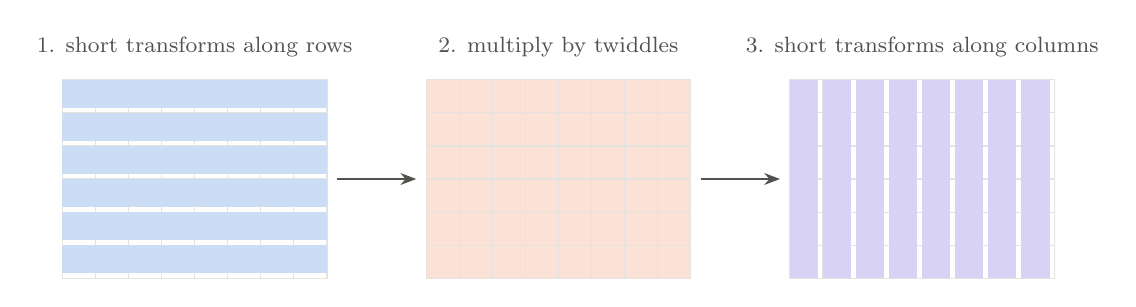
\begin{tikzpicture}[scale=0.42]
  \foreach \r in {0,...,5} \foreach \c in {0,...,7} \draw[rule,fill=white] (\c,-\r) rectangle +(1,-1);
  \foreach \r in {0,...,5} \fill[sBlue!25] (0,-\r) rectangle (8,-\r-0.85);
  \node[lbl] at (4,1) {1. short transforms along rows};
  \begin{scope}[shift={(11,0)}]
    \foreach \r in {0,...,5} \foreach \c in {0,...,7} \draw[rule,fill=sOrange!20] (\c,-\r) rectangle +(1,-1);
    \node[lbl] at (4,1) {2. multiply by twiddles};
  \end{scope}
  \begin{scope}[shift={(22,0)}]
    \foreach \r in {0,...,5} \foreach \c in {0,...,7} \draw[rule,fill=white] (\c,-\r) rectangle +(1,-1);
    \foreach \c in {0,...,7} \fill[sViolet!25] (\c,0) rectangle (\c+0.85,-6);
    \node[lbl] at (4,1) {3. short transforms along columns};
  \end{scope}
  \draw[arr] (8.3,-3) -- (10.7,-3);
  \draw[arr] (19.3,-3) -- (21.7,-3);
\end{tikzpicture}
\caption{The matrix method: one long transform becomes many short ones that fit in cache,
plus a twiddle pass and transposes.}
\end{figure}

Each short transform (at most $2^{13}$ entries, \code{BIGMATH\_NTT\_MFA\_LEAF}) fits in the
fastest cache, so the butterflies run at cache speed. BigMath goes further and
\emph{fuses} the transposes, the packing of input limbs, and even the pointwise
multiplication into these passes, so the second operand's transform never gets written to
memory at all. The method is used from transform length $2^{20}$
(\code{BIGMATH\_NTT\_MFA\_THRESHOLD}); at $2^{22}$ it made products 3 times faster.

\section{The power-of-two staircase and the $H + L$ trick}
\label{sec:trunc}

The transform length is a power of two at least as long as the product. A product needing
$c = 4100$ coefficients therefore uses length 8192: almost double the work of a product
needing 4096. Plotted against size, the cost is a staircase (\cref{fig:trunc}).

\begin{figure}[ht]
\centering
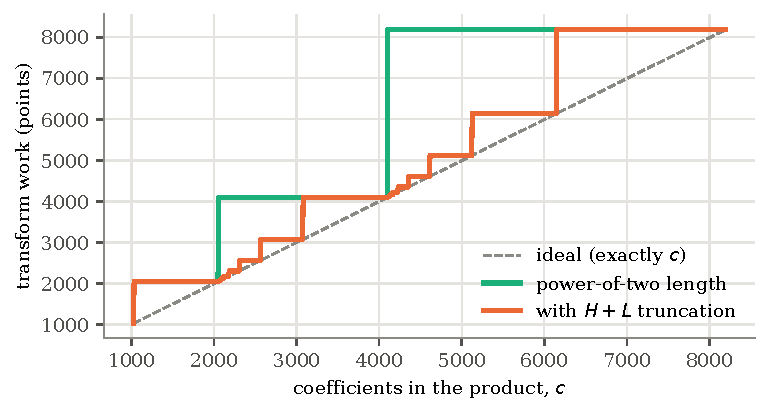
\includegraphics[width=0.8\textwidth]{figures/trunc_staircase.pdf}
\caption{Transform work against product size. Green: plain power-of-two lengths. Orange:
with the $H+L$ scheme, which fills in the steps just above each power of two (for
$2048 \le H \le 2^{20}$, up to $1.5H$). Computed from the length rules in the source.}
\label{fig:trunc}
\end{figure}

For a product just above a power of two $H$, BigMath computes it in two smaller pieces and
glues them together:

\begin{enumerate}
  \item The product \emph{modulo $x^H + 1$}, using a length-$H$ transform. (This is a
        ``negacyclic'' transform: coefficients that wrap around come back with a minus
        sign. It is a normal transform with the inputs pre-multiplied by powers of a
        $2H$-th root of unity; those weights are exactly the twiddle tables of the length-$2H$
        transform, so nothing new is needed.)
  \item The product \emph{modulo $x^L - 1$}, using a short cyclic transform of length $L$,
        the smallest power of two covering the overflow $c - H$.
\end{enumerate}

Because $x^H + 1$ and $x^L - 1$ share no factor, the two residues determine the product,
and a simple formula recovers it: if $C = C_{\text{lo}} + x^H C_{\text{hi}}$, the first
residue is $C_{\text{lo}} - C_{\text{hi}}$ and the second determines $C_{\text{hi}}$, so
$C_{\text{hi}} = (\text{second} - \text{folded first})/2$ and
$C_{\text{lo}} = \text{first} + C_{\text{hi}}$. Total transform work is $H + L$ instead of
$2H$.

\begin{center}
\small
\begin{tabular}{rrrrrr}
\toprule
$H$ & $c \approx H$ & $c = 1.0625H$ & $c = 1.125H$ & $c = 1.25H$ & full $2H$ \\
\midrule
$2^{13}$ & 87.7 & 90.5 & 95.7 & 103.7 & 143.5 \\
$2^{16}$ & 519.6 & 536.6 & 572.9 & 621.6 & 1\,132.6 \\
$2^{18}$ & 2\,891 & 3\,064 & 3\,657 & 3\,951 & 6\,839 \\
\bottomrule
\end{tabular}

\smallskip
{\footnotesize Microseconds per multiply, threaded, M1 Max.}
\end{center}

In single-threaded builds the scheme continues up to $H = 2^{25}$ for the whole octave,
processing one prime at a time to keep the working set small (0.45--0.88 times the full
transform's time). Multithreaded builds keep the full transform above $2^{20}$ because its
fused stages split better across cores.

\section{Using all the cores}
\label{sec:nttthreads}

A product needs six forward transforms (two operands times three primes), and they are
independent. BigMath runs them as six work units on its thread pool, then the pointwise
products, then the inverse transforms. Three inverse transforms would leave cores idle, so
each is split into two halves (a length-$N$ inverse is two length-$N/2$ inverses plus one
combining layer), giving six units again. Finally the carry pass is cut into per-thread
ranges: each range runs with carry-in zero and reports its carry-out, and a quick ripple
adds the carry-outs at the range boundaries.

\begin{figure}[ht]
\centering
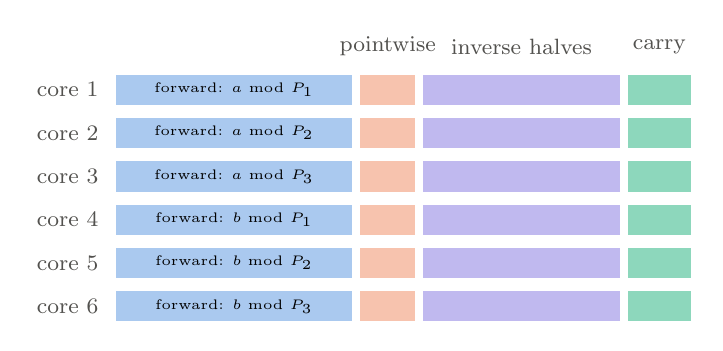
\begin{tikzpicture}[x=1cm,y=0.55cm]
  \foreach \t/\l in {0/$a$ mod $P_1$,1/$a$ mod $P_2$,2/$a$ mod $P_3$,3/$b$ mod $P_1$,4/$b$ mod $P_2$,5/$b$ mod $P_3$} {
    \node[lbl,anchor=east] at (-0.1,-\t) {core \the\numexpr\t+1\relax};
    \fill[sBlue!40] (0,-\t-0.35) rectangle (3,-\t+0.35);
    \node[font=\tiny] at (1.5,-\t) {forward: \l};
    \fill[sOrange!40] (3.1,-\t-0.35) rectangle (3.8,-\t+0.35);
    \fill[sViolet!40] (3.9,-\t-0.35) rectangle (6.4,-\t+0.35);
    \fill[sAqua!50] (6.5,-\t-0.35) rectangle (7.3,-\t+0.35);
  }
  \node[lbl] at (3.45,1) {pointwise};
  \node[lbl] at (5.15,1) {inverse halves};
  \node[lbl] at (6.9,1) {carry};
\end{tikzpicture}
\caption{Work units of one threaded NTT product: six forward transforms, pointwise
products, six inverse half-transforms, and a range-split carry pass.}
\end{figure}

Small transforms (under 2048 coefficients, \code{BIGMATH\_NTT\_PARALLEL\_MIN}) run on the
calling thread, because waking threads for a 25\,\textmu s product is not worth it. Larger
ones use up to eight threads (\code{BIGMATH\_MAX\_THREADS}). The result is bit-for-bit the
same whether one or eight threads run; threads change only the time.

\begin{center}
\small
\begin{tabular}{lrrr}
\toprule
transform length & serial-era original (\textmu s) & now, threaded (\textmu s) & speedup \\
\midrule
$2^{12}$ & 136 & 42 & 3.2$\times$ \\
$2^{16}$ & 1\,374 & 646 & 2.1$\times$ \\
$2^{20}$ & 24\,557 & 11\,358 & 2.2$\times$ \\
$2^{24}$ & 649\,997 & 443\,428 & 1.5$\times$ \\
\bottomrule
\end{tabular}
\end{center}

\section{Squares and reused operands}

\textbf{Squares.} When both operands are the same object, only three forward transforms are
needed instead of six, and the pointwise step squares each value. The square dispatcher
(\cref{sec:sqdispatch}) sends large squares here.

\textbf{Reused operands.} If you multiply many numbers by the same large number, its
transforms can be computed once:

\begin{lstlisting}
#include "biginteger/ops/Multiplication.h"
// Prepare once, for partners of up to 200000 limbs.
PreparedMultiplication pm = PrepareMultiplication(bigConstant, 200000);
for (auto const &x : values)
    results.push_back(pm * x);   // only x is transformed each time
\end{lstlisting}

Single-threaded this saved about a third of the time at $100\,000 \times 100\,000$ limbs; with
threads the gain is smaller (about 7\%), because the six forward transforms already run in
parallel.

\section{Summary of the NTT pipeline}

\begin{figure}[ht]
\centering
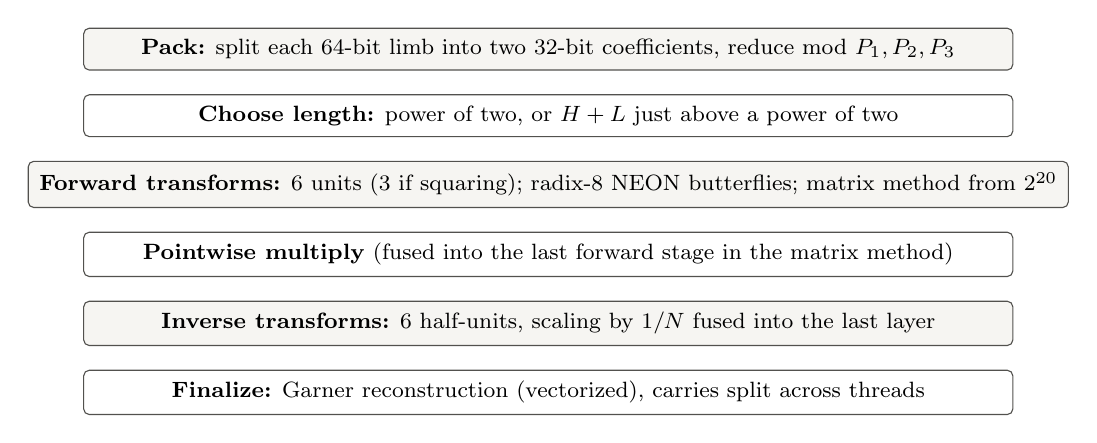
\begin{tikzpicture}[node distance=3mm,every node/.style={box,font=\footnotesize,minimum width=118mm,align=left}]
  \node[fill=paper] (s1) {\textbf{Pack:} split each 64-bit limb into two 32-bit coefficients, reduce mod $P_1, P_2, P_3$};
  \node[below=of s1] (s2) {\textbf{Choose length:} power of two, or $H + L$ just above a power of two};
  \node[fill=paper,below=of s2] (s3) {\textbf{Forward transforms:} 6 units (3 if squaring); radix-8 NEON butterflies; matrix method from $2^{20}$};
  \node[below=of s3] (s4) {\textbf{Pointwise multiply} (fused into the last forward stage in the matrix method)};
  \node[fill=paper,below=of s4] (s5) {\textbf{Inverse transforms:} 6 half-units, scaling by $1/N$ fused into the last layer};
  \node[below=of s5] (s6) {\textbf{Finalize:} Garner reconstruction (vectorized), carries split across threads};
\end{tikzpicture}
\caption{The whole NTT product, as implemented in \file{NTTMultiplicationCrt.h}.}
\end{figure}

\chapter{Multiplication III: Fermat FFT}
\label{ch:fermat}

A huge product can exceed the limits of a single wide CRT residue product.
One option is to cut each input into blocks, multiply every pair, and add the
overlapping results. BigMath also has an experimental path that transforms
the blocks first. It does fewer large inner products as the number of blocks
grows, at the cost of moving and mixing arrays of large values. The transform
is called \emph{outer} because the values it multiplies are themselves large
integers. BigMath uses its ordinary multiplier inside that step.

\begin{figure}[H]
\centering
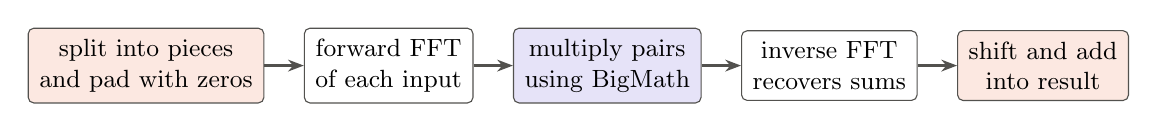
\begin{tikzpicture}[node distance=5mm]
  \node[box,fill=sOrange!15] (in) {split into pieces\\and pad with zeros};
  \node[box,right=of in] (forward) {forward FFT\\of each input};
  \node[box,fill=sViolet!16,right=of forward] (multiply) {multiply pairs\\using BigMath};
  \node[box,right=of multiply] (inverse) {inverse FFT\\recovers sums};
  \node[box,fill=sOrange!15,right=of inverse] (out) {shift and add\\into result};
  \draw[arr] (in) -- (forward);
  \draw[arr] (forward) -- (multiply);
  \draw[arr] (multiply) -- (inverse);
  \draw[arr] (inverse) -- (out);
\end{tikzpicture}
\caption{The outer FFT rearranges the chunk products. Each inner product
is reduced modulo $2^n+1$ before the inverse transform.}
\end{figure}

\section{Why this modulus makes shifts cheap}

All the arithmetic inside the outer FFT uses remainders modulo $M=2^n+1$.
In this arithmetic, $2^n$ is one less than $M$, so it acts like $-1$.
If you shift a value and some bits spill over position $n$, split at
that position and subtract the high part from the low part:
\[
\text{low}+2^n\cdot\text{high}
   \equiv \text{low}-\text{high}\pmod{2^n+1}.
\]

\begin{figure}[H]
\centering
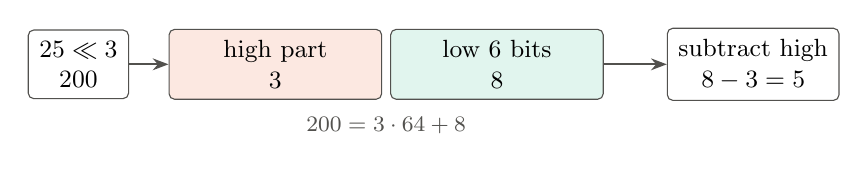
\begin{tikzpicture}[node distance=5mm]
  \node[box] (start) {$25\ll 3$\\$200$};
  \node[box,fill=sOrange!15,right=of start,minimum width=27mm] (high)
    {high part\\$3$};
  \node[box,fill=sAqua!13,right=1mm of high,minimum width=27mm] (low)
    {low 6 bits\\$8$};
  \node[box,right=8mm of low] (fold) {subtract high\\$8-3=5$};
  \draw[arr] (start) -- (high);
  \draw[arr] (low) -- (fold);
  \node[lbl,below=1mm of $(high.south)!0.5!(low.south)$] {$200=3\cdot64+8$};
\end{tikzpicture}
\caption{A shift by three bits followed by a fold, here modulo $65=2^6+1$.
If the subtraction is negative, add the modulus to get a nonnegative remainder.}
\end{figure}

Twiddle factors are the fixed multipliers in the butterfly steps
(\cref{ch:ntt}). The FFT chooses them to be powers of two, so applying one
is a shift and fold. A general pointwise product still requires the
ordinary multiplier. The implementation takes that full product and
folds its high half using the same subtraction. This style of exact FFT
uses integer remainders throughout. For the broader technique, see the
\href{https://gmplib.org/manual/FFT-Multiplication}{GNU MP manual on Fermat-style FFTs}.

\newpage
\section{A four-point product you can check by hand}

Multiply $13$ by $15$ in base 4, with one base-4 digit per piece. The inputs
are $(1,3)$ and $(3,3)$, low piece first. Choose four slots and fill the
unused input slots with zeros. The three sums that contribute to the
product occupy positions 0, 1, and 2, with room for all of them before
the transform's index would wrap back to 0.

\begin{figure}[H]
\centering
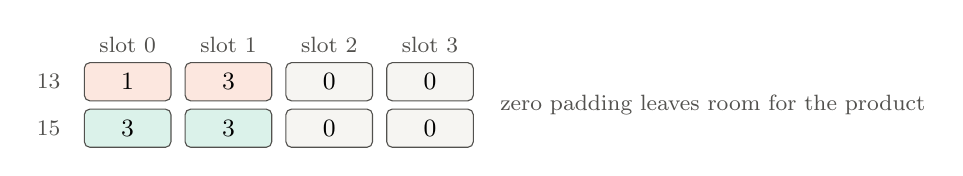
\begin{tikzpicture}[x=1.28cm,y=0.59cm]
  \foreach \i/\a/\b in {0/1/3,1/3/3,2/0/0,3/0/0} {
    \node[lbl] at (\i,1.55) {slot \i};
    \ifnum\i<2
      \node[box,minimum width=11mm,fill=sOrange!16] at (\i,0.75) {\a};
      \node[box,minimum width=11mm,fill=sAqua!16] at (\i,-0.25) {\b};
    \else
      \node[box,minimum width=11mm,fill=paper] at (\i,0.75) {\a};
      \node[box,minimum width=11mm,fill=paper] at (\i,-0.25) {\b};
    \fi
  }
  \node[lbl,anchor=east] at (-0.57,0.75) {$13$};
  \node[lbl,anchor=east] at (-0.57,-0.25) {$15$};
  \node[lbl,anchor=west] at (3.6,0.25) {zero padding leaves room for the product};
\end{tikzpicture}
\caption{The example uses four FFT slots. Their indices hold the powers of the piece
base after the inverse FFT recovers the coefficients.}
\end{figure}

Work modulo $65$. The four transform points are the powers of $8$:
$1,8,-1,-8$. They repeat after four steps because $8^2=64\equiv-1$ and
$8^4\equiv1$. Evaluate the two input recipes $1+3x$ and $3+3x$ at each point
and multiply the remainders.

\begin{center}
\small
\begin{tabular}{lrrrr}
\toprule
point & $1$ & $8$ & $-1$ & $-8$ \\
\midrule
$1+3x$ modulo $65$ & 4 & 25 & 63 & 42 \\
$3+3x$ modulo $65$ & 6 & 27 & 0 & 44 \\
pointwise product modulo $65$ & 24 & 25 & 0 & 28 \\
\bottomrule
\end{tabular}
\end{center}

At point 8, $25\cdot27=675=10\cdot64+35$. Folding gives $35-10=25$.
To undo the transform, weight each product by the inverse power of its
point, then divide the sum by four in the same modular arithmetic.
Here $4\cdot49\equiv1$, so division by four means multiplication by 49.
For example, the weights for coefficient 1 are $1,-8,-1,8$, giving
$24-8\cdot25+8\cdot28=48$ before scaling. These weights make four copies
of the coefficient we want. Contributions from the other coefficients
cancel, just as $1+8-1-8=0$.

\begin{center}
\small
\begin{tabular}{lrrrr}
\toprule
coefficient index & 0 & 1 & 2 & 3 \\
\midrule
weighted sum modulo $65$ & 12 & 48 & 36 & 0 \\
after multiplying by 49 modulo $65$ & 3 & 12 & 9 & 0 \\
\bottomrule
\end{tabular}
\end{center}

These are the integer coefficients. Each sums at most two products of
digits at most 3, so all are at most $18<65$. Now carry in base 4.
The $12$ at position 1 writes $0$ and sends $3$ to the $9$ at position 2.
That $12$ again writes $0$ and sends $3$ to position 3.
The resulting digits $(3,0,0,3)$ give $3+3\cdot4^3=195$.

\begin{figure}[H]
\centering
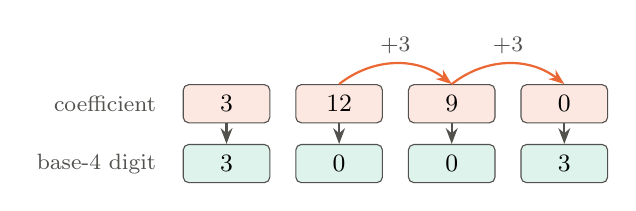
\begin{tikzpicture}[x=1.43cm,y=0.76cm]
  \foreach \i/\raw/\digit in {0/3/3,1/12/0,2/9/0,3/0/3} {
    \node[box,fill=sOrange!15,minimum width=11mm] (raw\i) at (\i,0) {\raw};
    \node[box,fill=sAqua!15,minimum width=11mm] (digit\i) at (\i,-1) {\digit};
    \draw[arr] (raw\i) -- (digit\i);
  }
  \node[lbl,anchor=east] at (-0.54,0) {coefficient};
  \node[lbl,anchor=east] at (-0.54,-1) {base-4 digit};
  \draw[arr,sOrange] (raw1.north) to[bend left=38] node[lbl,above] {$+3$} (raw2.north);
  \draw[arr,sOrange] (raw2.north) to[bend left=38] node[lbl,above] {$+3$} (raw3.north);
\end{tikzpicture}
\caption{Carry moves from low to high. A coefficient plus its incoming
carry supplies the digit below it and any carry to the next position.}
\end{figure}

\newpage
\section{How BigMath sets up a real product}
\label{sec:fermatparams}

Pieces in the library are whole runs of 64-bit limbs. Two choices make
the result exact.

\begin{enumerate}
  \item \textbf{Leave room for every position.} Choose a power-of-two number
        of slots $K=2^k$. With $a$ and $b$ limbs in the two operands, each
        piece holds $m=\ceil{(a+b)/(K-1)}$ limbs. The total number of output
        coefficients is one less than the sum of the input piece counts,
        and fits in $K$ slots.
  \item \textbf{Leave room for the value in each position.} A product of two
        $m$-limb pieces fits in $128m$ bits. Adding up to $K$ terms needs at
        most $k$ more bits. BigMath starts with $128m+k+1$ bits and rounds up
        to a multiple of $\max(64,K/2)$ for the modulus exponent $n$.
        That aligns residues to limb boundaries and makes $2^{2n/K}$ an
        available root for the FFT.
\end{enumerate}

The automatic selector starts at $k=6$ (64 slots) and takes the first fit
through $k=14$ with $n\le2^{28}$ bits. The forward and inverse FFTs share
the same shuffled slot order, saving a reordering pass. Large butterfly
layers use the pool. The caller does the pointwise products one at a time
so each inner multiplication can use that same pool. Each product reads the
significant limbs of its two residues in place. The caller can reuse the product
buffer at the next point after folding the result modulo $2^n+1$. For a square,
one forward transform serves both inputs. After the inverse FFT, add each
coefficient at its starting limb offset $im$, where $i$ is its position.
The coefficients can span several pieces, so the shifted additions
carry across their overlaps.

\section{When the dispatcher can use it}
\label{sec:fermatdispatch}

The build must use 64-bit limbs and the fused wide-CRT path. After both
CRT residue sets fail their size checks, the dispatcher
can try Fermat before splitting into overlap-add blocks
(\cref{sec:hugeproductdispatch}). It also checks the threshold
\code{BIGMATH\_NTT\_FERMAT\_MIN\_COEFFS}, counted in 32-bit product
coefficients, and checks whether the parameter selector found a fit.
The default threshold disables the path. See \file{FermatOuterMultiplication.h}.

\begin{table}[H]
\centering
\small
\begin{tabular}{lrrrr}
\toprule
Digits per input & \multicolumn{2}{c}{Warm time (s)} & \multicolumn{2}{c}{Peak RSS (GiB)} \\
\cmidrule(lr){2-3}\cmidrule(lr){4-5}
& Forced blocks & Fermat & Forced blocks & Fermat \\
\midrule
250 million & 3.39 & 2.88 & 1.49 & 1.71 \\
2.5 billion & 27.66 & 29.12 & 10.26 & 14.34 \\
5 billion & 55.65 & 77.79 & 19.30 & 20.12 \\
\bottomrule
\end{tabular}
\caption{Local comparisons on a 32\,GiB Apple M1 Max with up to eight
threads. Both modes were forced at these sizes. The forced-block control used
three blocks per input. Warm products matched GMP hashes. The 5-billion-digit
Fermat run incurred system swap.}
\end{table}

The crossover beyond the wide-CRT limits still needs measurements at
those sizes. The default build handles the balanced 2.5- and 5-billion-digit
cases in the table with single wide residue products. Full measurements and
reproduction commands are in \file{BENCHMARK.md}.

\chapter{Choosing a multiplication algorithm}
\label{ch:muldispatch}

\Cref{ch:mul,ch:ntt} described four methods. This chapter explains how
\code{Multiply} picks one. The implementation is in
\file{src/algorithms/Multiplication.cpp}.

\section{The decision, step by step}

\Cref{fig:muldispatch} shows the tests in the order the code applies them. The first one
matching the operands decides; the sections after the figures explain where each number
comes from.

\begin{figure}[tbp]
\centering
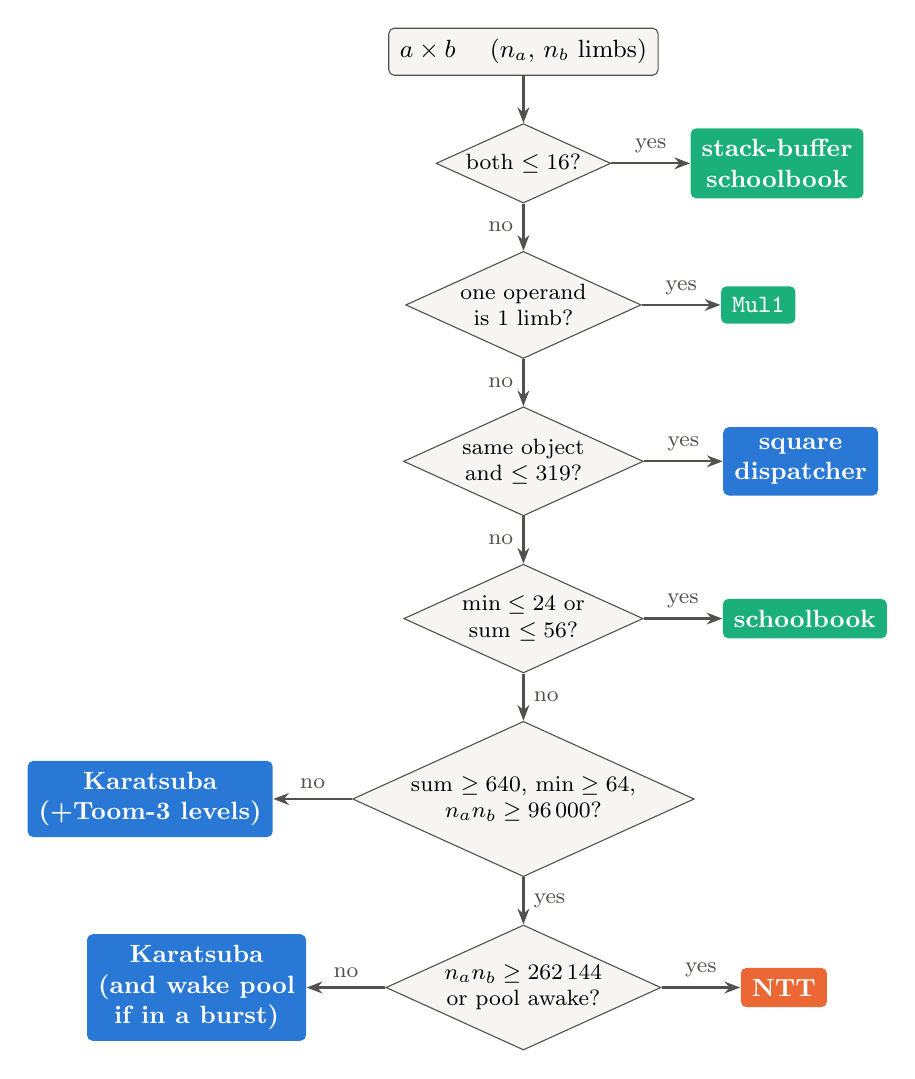
\begin{tikzpicture}[node distance=6mm and 10mm]
  \node[box,fill=paper] (start) {$a \times b$ \quad ($n_a$, $n_b$ limbs)};
  \node[dec,below=of start] (small) {both $\le 16$?};
  \node[algo,fill=sAqua,right=of small] (stack) {stack-buffer\\schoolbook};
  \node[dec,below=of small] (one) {one operand\\is 1 limb?};
  \node[algo,fill=sAqua,right=of one] (mul1) {\code{Mul1}};
  \node[dec,below=of one] (sq) {same object\\and $\le 319$?};
  \node[algo,fill=sBlue,right=of sq] (sqd) {square\\dispatcher};
  \node[dec,below=of sq] (cl) {$\min \le 24$ or\\sum $\le 56$?};
  \node[algo,fill=sAqua,right=of cl] (school) {schoolbook};
  \node[dec,below=of cl] (ntt) {sum $\ge 640$, $\min \ge 64$,\\$n_a n_b \ge 96\,000$?};
  \node[algo,fill=sBlue,left=of ntt] (kar) {Karatsuba\\(+Toom-3 levels)};
  \node[dec,below=of ntt] (cold) {$n_a n_b \ge 262\,144$\\or pool awake?};
  \node[algo,fill=sOrange,right=of cold] (nttx) {NTT};
  \node[algo,fill=sBlue,left=of cold] (kar2) {Karatsuba\\(and wake pool\\if in a burst)};
  \draw[arr] (start) -- (small);
  \draw[arr] (small) -- node[above,lbl]{yes} (stack);
  \draw[arr] (small) -- node[left,lbl]{no} (one);
  \draw[arr] (one) -- node[above,lbl]{yes} (mul1);
  \draw[arr] (one) -- node[left,lbl]{no} (sq);
  \draw[arr] (sq) -- node[above,lbl]{yes} (sqd);
  \draw[arr] (sq) -- node[left,lbl]{no} (cl);
  \draw[arr] (cl) -- node[above,lbl]{yes} (school);
  \draw[arr] (cl) -- node[right,lbl]{no} (ntt);
  \draw[arr] (ntt) -- node[above,lbl]{no} (kar);
  \draw[arr] (ntt) -- node[right,lbl]{yes} (cold);
  \draw[arr] (cold) -- node[above,lbl]{yes} (nttx);
  \draw[arr] (cold) -- node[above,lbl]{no} (kar2);
\end{tikzpicture}
\caption{The multiplication dispatcher with 64-bit limbs and generic thresholds.
The stack-buffer test happens in the operator layer.}
\label{fig:muldispatch}
\end{figure}

\Cref{fig:muldispmap} draws the same rules as a map over operand shapes. Each point is a
pair of lengths; its colour is the algorithm that runs.

\begin{figure}[ht]
\centering
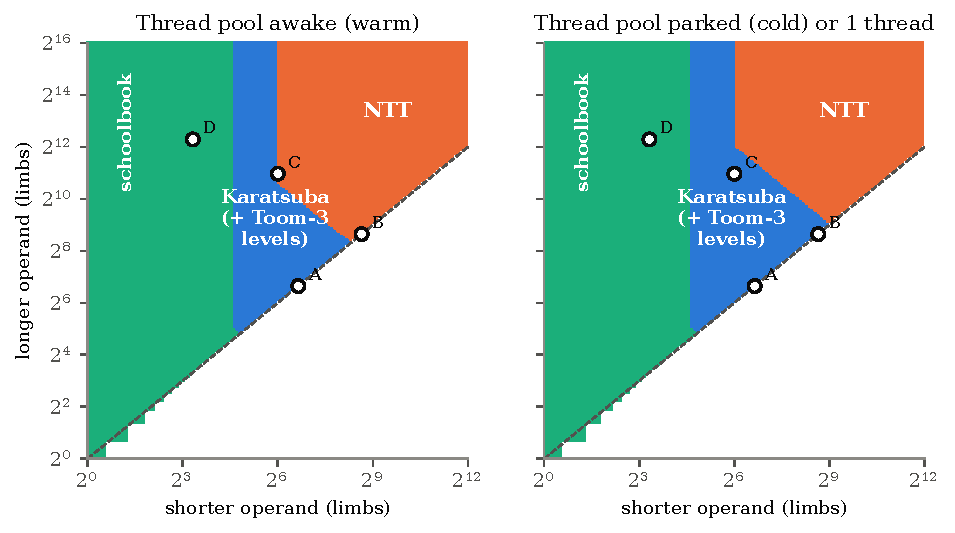
\includegraphics[width=\textwidth]{figures/mul_dispatch_map.pdf}
\caption{Which algorithm multiplies an $n_{\min} \times n_{\max}$ product, with the thread
pool awake (left) and parked or disabled (right), using the generic thresholds.
Points A--D are the worked examples in \cref{sec:mulexamples}.}
\label{fig:muldispmap}
\end{figure}

\section{Rule 1: schoolbook when the short operand is short}

Schoolbook runs when the shorter operand has at most 24 limbs, or both together have at most
56. The 24 is not a coincidence: it is the Karatsuba leaf size. If the shorter operand is
already at or below the leaf size, Karatsuba would just slice the long operand and hand every
piece to the schoolbook kernel anyway, so calling schoolbook directly skips the bookkeeping.

Note that this holds \emph{however long} the other operand is: $10 \times 100\,000$ limbs is a
schoolbook product. Its cost, $10 \times 100\,000$ limb products, is linear in the long
operand, and no fancier method can beat a single pass over the data by much.

\section{Rule 2: the NTT when the product is big \emph{in area}}
\label{sec:arearule}

For balanced products the NTT overtakes Karatsuba at about 310 limbs per operand. For
lopsided products the story is different, and this is where the shape map's slanted
boundary comes from.

Recall from \cref{sec:karatsuba} that sliced Karatsuba costs about
$n_{\max} \cdot K(n_{\min})/n_{\min}$: linear in the long operand, at a per-limb rate set by
the short one (measured 26\,ns per long-operand limb when $n_{\min} = 64$, 41\,ns at 128,
64\,ns at 256). The NTT's cost follows the \emph{total} length. So the shorter the short
operand, the longer the product must be before the NTT wins:

\begin{center}
\small
\begin{tabular}{rrr}
\toprule
shorter operand & NTT wins from (longer) & area $n_a n_b$ at crossover \\
\midrule
48 & never (at $48 \times 6144$: 139 vs 146\,\textmu s for Karatsuba) & --- \\
64 & $\approx$ 1500--2000 & 96k--128k \\
128 & $\approx$ 750 & 96k \\
160 & $\approx$ 630 & 101k \\
256 & $\approx$ 450 & 115k \\
balanced & 320 & 102k \\
\bottomrule
\end{tabular}
\end{center}

The crossover sits at a nearly constant \emph{area} $n_a \times n_b$, the number of limb
products schoolbook would need. That gives a simple rule with three conditions:
\[
n_a + n_b \ge 640, \qquad \min(n_a,n_b)\ge 64, \qquad n_a n_b \ge 96\,000.
\]
These generic floors make a product eligible for the NTT. The worker-state
rule below makes the final choice between the NTT and recursive multiplication.

\begin{another}
Think of the cost of each method as a surface over the $(n_{\min}, n_{\max})$ plane. The
dispatcher's job is to report which surface is lowest at each point. The boundaries in
\cref{fig:muldispmap} are where two surfaces cross. Measuring on a grid of shapes, not just
on balanced products, is what revealed that the Karatsuba/NTT boundary is a curve of
constant area rather than a line of constant total size.
\end{another}

\section{Rule 3: is the thread pool awake?}
\label{sec:poolrule}

The 96\,000 area threshold was measured with multiplications running back to back. In that
situation the pool's worker threads never fall asleep, and a small NTT spreads its six
transforms across six awake cores. An \emph{isolated} multiplication is different. Parked
threads take 20--30\,\textmu s to wake, which is as long as the whole product, so the
calling thread ends up doing nearly all the work itself.

\begin{figure}[ht]
\centering
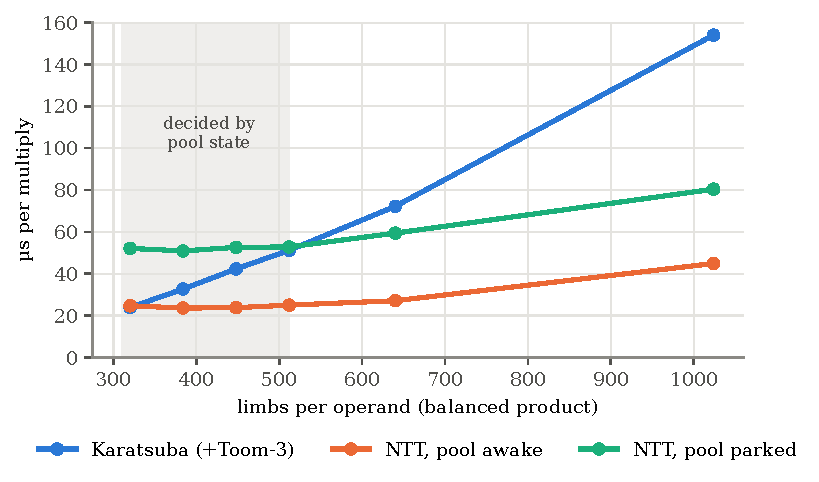
\includegraphics[width=0.8\textwidth]{figures/pool_temperature.pdf}
\caption{Time per balanced multiply. With the pool awake the NTT wins from about 320 limbs;
with the pool parked it costs about its serial time and only wins from about 512 limbs.
Data from \file{docs/MULTIPLICATION.md} (M1 Max).}
\label{fig:pool}
\end{figure}

So between area 96\,000 and 262\,144 ($\approx 512 \times 512$) the dispatcher asks the pool
whether it is awake. If yes, NTT; if not, Karatsuba. Above 262\,144 the NTT wins even cold.

There is one more twist. If a program does a \emph{burst} of mid-sized multiplications, the
first one finds the pool asleep and uses Karatsuba, which is right for it. But then every
later one would too, and the pool would never wake. To prevent this, a thread that finishes
two cold operations within 100\,\textmu s (\code{BIGMATH\_POOL\_SPIN\_US}) of each other
nudges the pool awake without giving it work. The third multiplication of the burst then
finds it warm and takes the NTT. An isolated multiplication wakes nothing.

\begin{practice}
Both paths compute the same exact product. With the generic profile,
\code{-DBIGMATH\_USE\_THREADS=0} uses the cold thresholds. The macOS Arm64
Clang profile adds a single-thread floor of 704 limbs for distinct operands
whose lengths differ by at most one limb. It leaves the threaded
worker-state rule in place.
\end{practice}

On the M1 Max, the one-thread recursive kernel took 40.0\,\textmu s
at $520\times520$ limbs, versus 46.5\,\textmu s for the NTT. At
$720\times720$, the NTT took 65.9\,\textmu s and recursion took
69.7\,\textmu s. The Apple silicon Clang kernel also specializes
schoolbook row widths from 12 through 24 limbs. Its NEON radix-8
butterflies reuse groups of twiddle factors and reduction constants
across blocks on short, repeated stages. See \file{BENCHMARK.md} for the
paired measurements through one million decimal digits.

\section{Squares}
\label{sec:sqdispatch}

When both operands are the same object (\code{x * x}) and have at most 319 limbs, the
multiplication goes straight to the square dispatcher, which exploits the symmetry of
\cref{sec:square}. Larger self-products go through the normal rules above. The ordinary
and truncated CRT transforms can reuse the spectrum of the shared operand
(\cref{sec:nttreuse}).

For a direct call to the square dispatcher, the generic thresholds are:

\begin{center}
\small
\begin{tabular}{ll}
\toprule
size (limbs) & square method \\
\midrule
1 & single-limb square \\
$< 48$ (inside Karatsuba square) & schoolbook square (\code{SqrBasecase}) \\
$48$--$351$ & Karatsuba square, Toom-3 levels from 160 \\
$352$--$607$ & NTT if the pool is awake, else Karatsuba square \\
$\ge 608$ & NTT self-product (see \cref{sec:nttreuse}) \\
\bottomrule
\end{tabular}
\end{center}

The profile can override the two NTT square floors
(\cref{sec:platformprofiles}). The ordinary CRT path saves three forward
transforms by reusing one spectrum per prime.

\section{Worked dispatch examples}
\label{sec:mulexamples}

\begin{example}[s: which algorithm runs?]
\begin{description}[leftmargin=1.2cm,style=nextline]
  \item[A: $100 \times 100$] Shorter operand $100 > 24$ and sum $200 > 56$: not schoolbook.
        Sum $200 < 640$: not NTT. $\Rightarrow$ \textbf{Karatsuba}. Its pieces (50, then 25)
        are below 168, so no Toom-3 level; the 25-limb pieces split once more to 13, which is
        under 24, so schoolbook leaves.
  \item[B: $400 \times 400$] Sum 800, minimum 400, area 160\,000: passes all three NTT tests.
        Area is below 262\,144, so it depends on the pool: \textbf{NTT} if awake (about
        24\,\textmu s), \textbf{Karatsuba} with a Toom-3 top level if parked (about 35\,\textmu s,
        better than a cold NTT's 51\,\textmu s).
  \item[C: $64 \times 2000$] Minimum 64 passes, sum 2064 passes, area 128\,000 passes.
        Warm: \textbf{NTT}. Cold: \textbf{Karatsuba}, slicing the long operand into 32 balanced
        $64 \times 64$ products.
  \item[D: $10 \times 5000$] Shorter operand $10 \le 24$: \textbf{schoolbook}, ten
        \code{AddMul1} rows over 5000 limbs.
  \item[E: $600 \times 600$] Area 360\,000 $\ge$ 262\,144: \textbf{NTT} regardless of the pool.
        The product has $2 \cdot 2 \cdot 600 = 2400$ coefficients, just above $H = 2048$, so the
        $H + L$ scheme runs with $L = 512$: transform work 2560 instead of 4096.
\end{description}
\end{example}

\section{How the rules were found}

The generic thresholds were re-measured on 20--21 November 2026, after the limb kernels,
Karatsuba slicing, and NTT improvements had all moved the crossovers. The procedure:
time every algorithm directly on a grid of shapes ($n_{\min}$ from 8 to 256 limbs,
ratios 1 to 128), find where each pair crosses, and fit the simplest rule that matches.
After the change the largest remaining mis-routes were near-ties within 17\% of the best
method.

\begin{perfnote}
End-to-end effect of that re-sweep, through the public API (M1 Max, warm):
multiplying two 20\,000-digit numbers went from 0.219\,ms to 0.048\,ms (4.6$\times$), and
from 2.7 times GMP's time to 0.6 times. 1\,000\,000-digit parsing and printing became
1.8 times faster without any change to their own code, because they are built on
\code{Multiply}.
\end{perfnote}

\chapter{Division I: short and long division}
\label{ch:div}

Division is harder than multiplication. Multiplying needs no guessing; dividing does. In
long division on paper you look at the leading digits, \emph{guess} the next quotient digit,
multiply back, and correct the guess if it was wrong. Every division algorithm in BigMath is
a refinement of that loop: make the guess cheaper, make it more accurate, or guess many
digits at once.

Given $a$ and $b > 0$, division produces a quotient $q$ and remainder $r$ with
\[
a = q \cdot b + r, \qquad 0 \le r < b .
\]
The tests check exactly this identity for every algorithm and every result.

\section{Dividing by a single limb}
\label{sec:shortdiv}

When the divisor fits in one limb, division is ``short division'': walk from the top limb
down, keeping a running remainder.

\begin{example}[: $9\,876 \div 7$ by short division]
\[
\begin{array}{l@{\qquad}l}
9 \div 7 = 1 \text{ rem } 2 & \\
(2\cdot 10 + 8) = 28 \div 7 = 4 \text{ rem } 0 & \\
(0 \cdot 10 + 7) = 7 \div 7 = 1 \text{ rem } 0 & \\
(0 \cdot 10 + 6) = 6 \div 7 = 0 \text{ rem } 6 & \Rightarrow\ q = 1410,\ r = 6 .
\end{array}
\]
In the library each step divides a two-limb value (remainder, next limb) by the one-limb
divisor.
\end{example}

The step ``divide a two-limb number by a one-limb number'' is the bottleneck: hardware
division of a 128-bit number is slow, or (on ARM) does not exist and becomes a library call.
But the divisor is the same at every step, so BigMath pays for one division up front and
then only multiplies.

\subsection{Dividing by multiplying with a precomputed reciprocal}

\begin{another}[: dividing by 7 without dividing]
To divide many numbers by 7, work out $1/7 \approx 0.14$ once. Then:
\begin{itemize}
  \item $93 \times 0.14 = 13.02$, guess $q = 13$; check $93 - 13 \cdot 7 = 2$, which is
        less than 7, so $q = 13$, $r = 2$.
  \item $98 \times 0.14 = 13.72$, guess $q = 13$; check $98 - 91 = 7$, which is \emph{not} less
        than 7, so correct once: $q = 14$, $r = 0$.
\end{itemize}
The guess may be slightly low, but a cheap check-and-correct step fixes it. Multiplication
replaced division.
\end{another}

The library uses the Möller--Granlund method (2011), which makes this exact for limbs: from
the divisor $d$ it precomputes $v = \floor{(B^2 - 1)/d} - B$. Each step is then one
$64 \times 64 \to 128$ multiplication, a few additions, and at most two small corrections.
Before the precomputation the divisor is \emph{normalized}: shifted left so its top bit is set.
\code{ClassicDivision::DivRem1} keeps the running remainder in that shifted form throughout and
shifts each dividend limb on the fly, so nothing is shifted back and forth on the critical
path.

\begin{perfnote}
Replacing the 128-bit hardware/library division with the reciprocal made printing small
numbers 2.1 times faster (printing divides by $10^{19}$ repeatedly). Keeping the remainder
normalized brought the per-limb cost from 6.4 to 4.9\,ns.
\end{perfnote}

\section{Normalization}
\label{sec:normalize}

Long division needs a good guess for each quotient digit, and the guess is made from the
leading digits. If the divisor's leading digit is tiny, the guess can be far off: dividing by
$10\ldots$ looks the same as dividing by $19\ldots$ when you only see one digit. The fix is to
scale both numbers so the divisor's leading digit is large.

\begin{keyidea}
Shift the dividend and divisor left by the same number of bits so the divisor's top limb has
its highest bit set. The quotient does not change (both were scaled by the same factor), the
remainder comes out scaled and is shifted back at the end. After normalization, a
quotient-digit guess from the leading limbs is never too small and at most two too large
(Knuth's theorem).
\end{keyidea}

In base 10 the equivalent is ``multiply both numbers so the divisor's first digit is at
least 5''.

\section{Long division: Knuth's Algorithm D}
\label{sec:knuth}

For divisors of 2 to 95 limbs BigMath uses classic long division in the form Donald Knuth
wrote down as ``Algorithm D''. Each round:

\begin{enumerate}
  \item \textbf{Guess} the next quotient digit $\hat q$ from the top of the current remainder.
  \item \textbf{Multiply and subtract}: remainder $\mathrel{-}= \hat q \cdot b$, shifted to the
        current position. This is one call of the \code{SubMul1} kernel.
  \item \textbf{Correct}: if the result went negative, the guess was one too big; add $b$
        back and decrement $\hat q$.
\end{enumerate}

\begin{example}[: $7369 \div 47$, the way Algorithm D does it]
\textbf{Normalize.} $47$ starts with 4; multiply both by 2: divide $14738$ by $94$.

\textbf{Round 1.} Window $147$. Guess from the leading digits: $14 \div 9 = 1$.
$147 - 1 \times 94 = 53$. Digit: 1.

\textbf{Round 2.} Bring down 3: window $533$. Guess $53 \div 9 = 5$.
$533 - 5 \times 94 = 63$. Digit: 5.

\textbf{Round 3.} Bring down 8: window $638$. Guess $63 \div 9 = 7$. But
$7 \times 94 = 658 > 638$: the guess was too big. Correct: digit 6, remainder
$638 - 564 = 74$.

\textbf{Un-normalize.} Quotient $156$; remainder $74 \div 2 = 37$.

Check: $47 \times 156 + 37 = 7332 + 37 = 7369$.
\end{example}

\subsection{A better guess: the 3-by-2 quotient digit}

In round 3 above the guess was wrong because it only looked at two digits of the remainder
and one of the divisor. Looking at \emph{three} digits of the remainder and \emph{two} of the
divisor gives $638 \div 94 = 6$: correct immediately. BigMath does exactly that with limbs. It
divides the top three limbs of the remainder by the top two limbs of the divisor, using a
Möller--Granlund \emph{3-by-2} reciprocal precomputed once per division. The guess is then
almost always exact; it is at most one too big, and that happens with probability about
$2/B \approx 10^{-19}$, so the add-back branch practically never runs.

\begin{perfnote}
The library's division loop used to be
\begin{lstlisting}
ULong128 product = (ULong128)v[i] * qhat + borrow;
if (u[j + i] < (DataT)product) { ...borrow... }   // a branch per limb
\end{lstlisting}
with a limb-sized borrow chain and an unpredictable branch on every limb: 2.9--4.0 cycles per
limb. The \code{SubMul1} kernel uses the two-chain layout of \cref{sec:flagchain}: products
along one chain, subtraction along another, no branches: 1.6--1.8 cycles per limb, level with
GMP's assembly from 128 limbs. The routine also works on raw buffers: both operands are
shifted into one workspace (on the stack up to 192 limbs), so a division allocates only its
two results. Divisions with 2- to 256-limb divisors got 1.7 to 2.5 times faster.
\end{perfnote}

\subsection{Cost}

Each quotient limb costs one pass over the divisor, so dividing an $n_a$-limb number by an
$n_b$-limb number costs about $(n_a - n_b + 1) \times n_b$ limb operations. That is fine for a
short divisor or a short quotient, but for two 10\,000-limb numbers with a 10\,000-limb
quotient it is 100 million operations. \Cref{ch:fastdiv} shows how to turn division into a
handful of multiplications instead.

\begin{practice}
For a one-limb divisor, use the scalar overloads (\code{a / uint64\_t}, \code{a \% uint64\_t}):
they go straight to \code{DivRem1}. If you need many divisions by the same multi-limb divisor,
see \code{CachedDivision} in \cref{sec:cached}.
\end{practice}

\chapter{Division II: turning division into multiplication}
\label{ch:fastdiv}

Long division costs (quotient length) $\times$ (divisor length). The methods in this chapter
reduce division to a small number of multiplications, so that division automatically
inherits Karatsuba, Toom-3 and the NTT. There are three ideas:

\begin{description}[leftmargin=2.8cm,style=sameline]
  \item[Burnikel--Ziegler] Do long division, but with each ``digit'' a large block, and the
        block steps done recursively.
  \item[Newton] Compute $1/b$ once, very accurately; then $a/b$ is $a \times (1/b)$ plus a
        small correction.
  \item[Top limbs] When the quotient is short, only the leading limbs of $a$ and $b$ matter.
\end{description}

\section{Burnikel--Ziegler: long division with big digits}
\label{sec:bz}

Go back to the long division of \cref{sec:knuth}, but imagine the ``digits'' are blocks of
many limbs. Each round still guesses a quotient block, multiplies it back, and corrects. The
guessing step is itself a division, of a smaller size, so it can be done by the same method,
recursively. The multiply-back step is a block-by-block multiplication, so it uses the fast
multipliers. This is Christoph Burnikel and Joachim Ziegler's recursive division (1998).

\subsection{One level of the recursion}

Split the normalized divisor into a high and a low half, $d = d_{\text{hi}} X + d_{\text{lo}}$.
To divide a $2n$-limb number by the $n$-limb $d$, compute the quotient in two halves. For each
half:

\begin{enumerate}
  \item Divide the top of the current remainder by $d_{\text{hi}}$ \emph{only}. This is a
        half-size division, done recursively. It gives a quotient guess $\hat q$ and a partial
        remainder.
  \item Subtract $\hat q \cdot d_{\text{lo}}$, the part of the divisor that step 1 ignored. This is
        one half-size multiplication.
  \item If the result is negative, the guess was too big: add $d$ back and decrement $\hat q$.
        Because $d$ is normalized, this happens at most a couple of times.
\end{enumerate}

\begin{example}[: $31\,415\,926 \div 5678$ with two-digit blocks]
The divisor $5678$ is normalized (leading digit $\ge 5$). Its halves are
$d_{\text{hi}} = 56$, $d_{\text{lo}} = 78$. The quotient will have two 2-digit blocks.

\textbf{High block.}
\begin{itemize}
  \item Divide the top four digits by $d_{\text{hi}}$: $3141 \div 56 = 56$ remainder $5$.
  \item Bring down the next block (59) and subtract $\hat q \cdot d_{\text{lo}}$:
        $5 \cdot 100 + 59 - 56 \times 78 = 559 - 4368 = -3809$.
  \item Negative, so add $d$ back: $-3809 + 5678 = 1869$, and $\hat q = 55$.
\end{itemize}

\textbf{Low block.}
\begin{itemize}
  \item Divide $1869$ by $d_{\text{hi}}$: $1869 \div 56 = 33$ remainder $21$.
  \item Bring down the last block (26): $21 \cdot 100 + 26 - 33 \times 78 = 2126 - 2574 = -448$.
  \item Negative: $-448 + 5678 = 5230$, and $\hat q = 32$.
\end{itemize}

Result: $q = 5532$, $r = 5230$. Check: $5532 \times 5678 + 5230 = 31\,410\,696 + 5230 = 31\,415\,926$.

Every step used a division of half the size ($4 \div 2$ digits) and a multiplication of half
the size ($2 \times 2$ digits). With large blocks those become recursive divisions and
Karatsuba or NTT products.
\end{example}

\begin{figure}[ht]
\centering
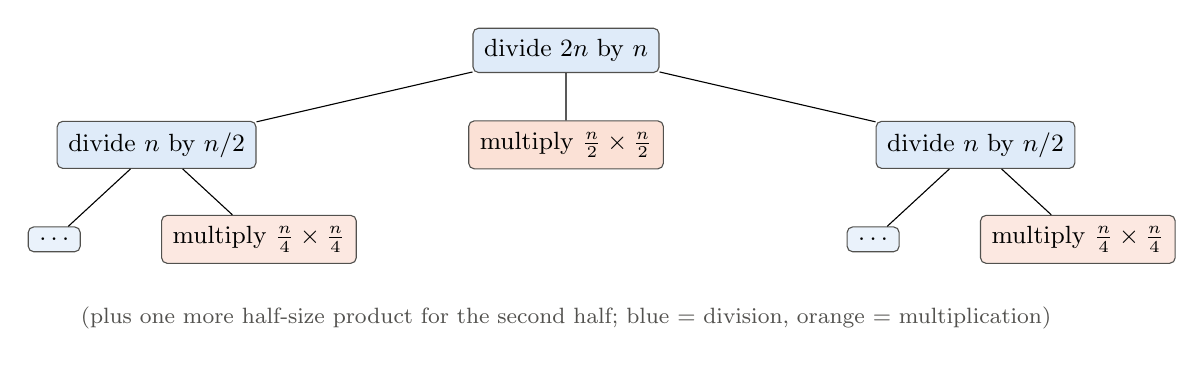
\begin{tikzpicture}[level distance=12mm,
  level 1/.style={sibling distance=52mm},
  level 2/.style={sibling distance=26mm},
  every node/.style={font=\footnotesize}]
  \node[box,fill=sBlue!15] {divide $2n$ by $n$}
    child {node[box,fill=sBlue!15] {divide $n$ by $n/2$}
      child {node[box,fill=sBlue!10] {$\ldots$}}
      child {node[box,fill=sOrange!15] {multiply $\tfrac n4\times\tfrac n4$}}}
    child {node[box,fill=sOrange!20] {multiply $\tfrac n2 \times \tfrac n2$}}
    child {node[box,fill=sBlue!15] {divide $n$ by $n/2$}
      child {node[box,fill=sBlue!10] {$\ldots$}}
      child {node[box,fill=sOrange!15] {multiply $\tfrac n4\times\tfrac n4$}}};
  \node[lbl] at (0,-3.4) {(plus one more half-size product for the second half; blue = division, orange = multiplication)};
\end{tikzpicture}
\caption{Burnikel--Ziegler recursion: two half-size divisions and two half-size
multiplications per level. The recursion bottoms out in Algorithm D at 64 limbs.}
\end{figure}

\paragraph{Cost.} $T(n) = 2\,T(n/2) + 2\,\M(n/2)$, which works out to about $\M(n) \log n$: a
logarithmic factor more than one multiplication, but far less than long division's $n^2$.

\paragraph{BigMath's version.} The implementation follows the in-place shape of GMP's
\code{mpn\_dcpi1\_div\_qr}. It works directly inside the shifted dividend buffer; the halves of
the divisor are just pointer offsets, not copies. An odd length splits into unequal halves,
so no zero padding is needed. A dividend longer than $2n$ is processed block by block from the
top. Recursion stops at 64 limbs (\code{BIGMATH\_DC\_DIV\_THRESHOLD}) and finishes with
Algorithm D.

\begin{pitfall}
The previous version copied operands into fresh vectors at every level and padded the divisor
with zero limbs so it halved evenly. Rewriting it in place made it 1.5--2.4 times faster. An
even older version had a worse problem: for odd divisor sizes it silently fell back to
quadratic long division one level down, costing 1.3--10 times on about half of all sizes.
\end{pitfall}

A useful property: when the quotient is shorter than the divisor, the recursion only uses
the divisor's top limbs plus one multiplication by the rest. So Burnikel--Ziegler already
costs about what ``quotient-sized'' division (below) costs for thin quotients.

\section{Newton's method: computing $1/b$}
\label{sec:newton}

\subsection{The idea, with ordinary numbers}

Newton's method finds $1/d$ using only multiplication and subtraction. Start from a rough
guess $x_0$ and repeat
\[
x_{k+1} = x_k \,(2 - d\, x_k) .
\]
If $x_k$ is close to $1/d$, the error of $x_{k+1}$ is about $d$ times the \emph{square} of the
error of $x_k$. So the number of correct digits roughly \emph{doubles} with every step.

\begin{example}[: $1/7$ from a guess of 0.1]
\begin{center}
\begin{tabular}{rlll}
\toprule
$k$ & $x_k$ & $7\,x_k$ & error $1/7 - x_k$ \\
\midrule
0 & 0.1 & 0.7 & $4.3 \times 10^{-2}$ \\
1 & $0.1\,(2 - 0.7) = 0.13$ & 0.91 & $1.3 \times 10^{-2}$ \\
2 & $0.13\,(2 - 0.91) = 0.1417$ & 0.9919 & $1.2 \times 10^{-3}$ \\
3 & $0.1417\,(2 - 0.9919) = 0.14284777$ & 0.99993439 & $9.4 \times 10^{-6}$ \\
4 & $0.142857142\ldots$ & & $6.1 \times 10^{-10}$ \\
\bottomrule
\end{tabular}
\end{center}
The true value is $0.142857142857\ldots$; correct digits go 1, 2, 3, 5, 9, 18, \ldots
(\cref{fig:newton}).
\end{example}

\begin{figure}[ht]
\centering
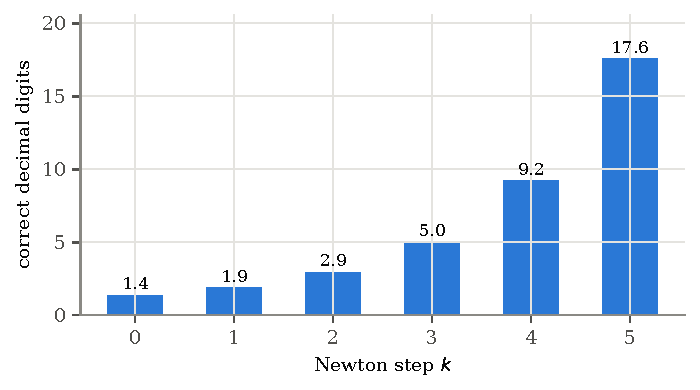
\includegraphics[width=0.7\textwidth]{figures/newton_convergence.pdf}
\caption{Correct digits of $1/7$ after each Newton step, starting from $0.1$. Each step
roughly doubles them. Computed with exact fractions by \file{figures/make\_figures.py}.}
\label{fig:newton}
\end{figure}

\subsection{Why the whole computation costs about two multiplications}

Because accuracy doubles each step, the early steps only need low precision. To get $n$
limbs, the last step works with $n$ limbs, the one before with $n/2$, the one before that
with $n/4$, and so on. The costs form a halving series: $\M(n) + \M(n/2) + \M(n/4) + \dots$,
which adds up to less than $2\,\M(n)$ for each multiplication in a step. Getting the
reciprocal costs a small constant number of full-size multiplications, not $\log n$ of them.

\subsection{In integers}

The library never uses fractions. For an $n$-limb normalized divisor $D$ it computes an
integer $R$ approximating $B^{2n}/D$, which is $1/D$ ``scaled up'' by $B^{2n}$. BigMath's
\code{ApproxReciprocal} guarantees
\[
0 \le \floor{B^{2n}/D} - R \le 3 ,
\]
that is, $R$ is never too large and at most 3 too small.

Two details make this work cheaply:

\begin{itemize}
  \item \textbf{A guarded precision schedule.} A Newton step on a $p$-limb estimate gives
        \emph{almost} $2p$ limbs, a few bits short. If each step asks for exactly double, the
        shortfall doubles too, and the final result can be off by a lot. BigMath instead works
        out the precisions \emph{backwards} from $n$: each earlier precision is
        $\ceil{(p + 2)/2}$, so each step has two guard limbs to spare. The first estimate is an
        exact reciprocal of the divisor's top (at most 32) limbs, computed with long division.
        This removed an extra full-size ``cleanup'' iteration the old code needed.
  \item \textbf{Only the new limbs are computed.} A step can be rewritten as
        ``old value, shifted, plus a correction'', where the correction depends on a small error
        term. Only the top limbs of the correction product are needed, so the step multiplies
        shorter numbers than the textbook formula.
\end{itemize}

\subsection{From the reciprocal to the quotient}

With $R \approx B^{2n}/D$ in hand, dividing a chunk of at most $2n$ limbs is:

\begin{enumerate}
  \item \textbf{Estimate}: $\hat q = \floor{\text{(top limbs of the chunk)} \times R / B^{2n}}$,
        one multiplication. Only the top $n+1$ limbs of the chunk can affect $\hat q$ (the rest
        contributes less than one unit), so only those are multiplied.
  \item \textbf{Remainder}: $r = \text{chunk} - \hat q \cdot D$, a second multiplication.
  \item \textbf{Fix up}: $\hat q$ is at most a few units too small; while $r \ge D$, subtract $D$
        and increase $\hat q$.
\end{enumerate}

\begin{figure}[ht]
\centering
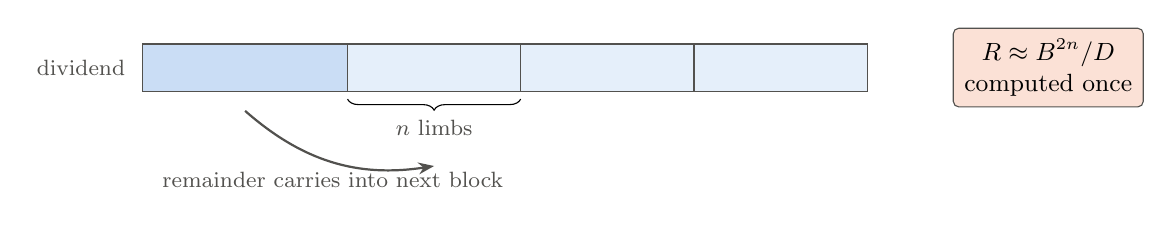
\begin{tikzpicture}[x=1cm,y=1cm]
  \fill[sBlue!25,draw=ink2] (0,0) rectangle (2.6,0.6) node[midway,font=\footnotesize] {leading chunk};
  \foreach \k in {1,2,3} \fill[sBlue!12,draw=ink2] ({2.6+(\k-1)*2.2},0) rectangle +(2.2,0.6) node[midway,font=\footnotesize] {block \k};
  \node[lbl,anchor=east] at (-0.1,0.3) {dividend};
  \draw[decorate,decoration={brace,amplitude=4pt,mirror}] (2.6,-0.1) -- (4.8,-0.1) node[midway,below=4pt,lbl] {$n$ limbs};
  \draw[arr] (1.3,-0.25) to[bend right=25] node[below,lbl] {remainder carries into next block} (3.7,-0.95);
  \node[box,fill=sOrange!20] at (11.5,0.3) {$R \approx B^{2n}/D$\\computed once};
\end{tikzpicture}
\caption{Blockwise Newton division: the reciprocal is computed once and reused for every
block of the dividend. Each block's remainder becomes the top of the next block.}
\end{figure}

For a long dividend the library processes it in blocks of $n$ limbs from the top, carrying
each remainder into the next block, and reusing the same $R$ throughout. The cost is the
reciprocal (a few $\M(n)$) plus about two $\M(n)$ per block. The more blocks there are, the
more the reciprocal is amortized: this is why Newton wins for lopsided divisions.

\subsection{The wrap-around remainder}
\label{sec:wrap}

Step 2 computes the full product $\hat q \cdot D$, about $2n$ limbs, only to subtract it from
the chunk and get a remainder that is known to be small (less than a few times $D$, so about
$n + 1$ limbs). Most of the product cancels.

Here the wrap-around of \cref{ch:ntt} becomes useful. A cyclic transform of length $L$
computes the product modulo $B^L - 1$ at about half the cost of the full product. If
$L \ge n + 2$, the remainder is small enough to be recovered exactly from
$(\text{chunk} - \hat q D) \bmod (B^L - 1)$, and whether it is negative can be read from its
size. The same trick computes the error term inside the reciprocal's Newton steps. Each of
these changes (wrapped remainder, wrapped reciprocal error, multiplying only the chunk's top
limbs) cut 10--25\% from large one-off divisions; together they took a 5-million by
1-million-digit division from 206\,ms to 111\,ms.

\subsection{Small leading blocks go to long division}

A dividend of exactly $k \cdot n$ limbs often gains one limb when it is normalized. That
leading block then has a one-limb quotient, but a full Newton chunk would cost two $n$-limb
multiplications to produce it. Leading blocks with at most 32 quotient limbs
(\code{BIGMATH\_NEWTON\_SCHOOLBOOK\_HEAD}) go to Algorithm D instead, which costs about 1.3\,ns
per divisor limb per quotient limb against 60--75\,ns for a chunk.

\begin{pitfall}
If a Newton quotient estimate is ever off by more than the fix-up loop allows, the code
falls back to long division. The answer is still correct, just quadratic, so nothing in the
correctness tests would notice. Once, a too-tight error bound in the reciprocal triggered
this fallback on every divide inside \code{ToString}, an 8-fold slowdown that was invisible
except in timings. \code{NewtonDivision::FallbackCount()} now counts fallbacks and the unit
tests assert it stays at zero.
\end{pitfall}

\section{Short quotients: only the top limbs matter}
\label{sec:toplimbs}

Suppose $a$ has 10\,010 limbs and $b$ has 10\,000. The quotient has only 11 limbs. Does
computing it really need all 20\,010 input limbs? No. A short quotient is decided by the
leading limbs of the operands; the rest can only move it by a tiny fraction.

\begin{example}[: estimating a quotient from the leading digits]
$a = 98\,765\,432\,198$ and $b = 123\,456\,789$. The quotient has about $11 - 9 + 1 = 3$ digits.
Keep the quotient length plus two guard digits of $b$, that is 4 digits, and the matching
digits of $a$:
\[
a' = 987\,654, \qquad b' = 1234, \qquad a' \div b' = 800 \text{ remainder } 454 .
\]
The true answer: $123\,456\,789 \times 800 = 98\,765\,431\,200$, remainder $998$. So $q = 800$,
found from a 6-digit by 4-digit division.
\end{example}

BigMath uses this in two places.

\paragraph{Quotient only (\code{a / b}).} When you ask only for the quotient and it is shorter
than the divisor, the dispatcher keeps $t = \delta + 4$ top limbs of $b$ (where
$\delta = n_a - n_b$) and the matching top limbs of $a$, and divides those. A short argument
shows the true quotient is either $q'$ or $q' - 1$, and it is $q'$ whenever the top remainder
$r'$ is at least $B^{\delta + 2}$, which for random inputs fails with probability about
$2^{-128}$. Only in that rare case (or when $a$ is an exact multiple of $b$, which always lands
there) is one $\delta \times n_b$ product computed to decide. The work drops from
$\delta \times n_b$ to a $(2\delta + 4)$-by-$(\delta + 4)$ division.

\begin{center}
\small
\begin{tabular}{rrrrr}
\toprule
divisor limbs & quotient limbs & before (\textmu s) & now (\textmu s) & GMP \code{mpz\_tdiv\_q} \\
\midrule
512 & 11 & 3.56 & 0.29 & 0.17 \\
1024 & 103 & 44.0 & 7.27 & 3.97 \\
4096 & 83 & 89.7 & 4.94 & 2.74 \\
16384 & 329 & 332 & 47.3 & 25.7 \\
\bottomrule
\end{tabular}
\end{center}

\paragraph{Quotient-sized division (with remainder).} When the remainder is also wanted and the
quotient is long (at least 3072 limbs) but still shorter than the divisor,
\code{QuotientSizedDivision} divides the operand tops (with Newton for large sizes), then
computes the remainder with one $\delta \times n_b$ multiplication and a few corrections. Its
cost scales with the \emph{quotient}, not the divisor.

\section{Reusing a divisor}
\label{sec:cached}

The reciprocal is the expensive part of Newton division, and it depends only on the divisor.
If you divide many numbers by the same divisor, compute it once:

\begin{lstlisting}
#include "biginteger/ops/Division.h"
CachedDivision div = CacheDivision(modulus);   // computes and stores the reciprocal
for (auto const &x : values) {
    auto [q, r] = div.DivideAndRemainder(x);    // reuses it every time
}
\end{lstlisting}

For five divisions by the same large divisor, the cached form measured 27--31 times faster
than five independent divisions (12--25 times including the one-time setup). Decimal printing
(\cref{ch:conv}) is built on exactly this.

\chapter{Choosing a division algorithm}
\label{ch:divdispatch}

Division has two size parameters: how long the divisor is ($n_b$ limbs) and how long the
quotient is ($\delta + 1$ limbs, where $\delta = n_a - n_b$). The best method depends on both.
The rules are in \file{src/algorithms/Division.cpp}; the numbers in
\file{include/biginteger/build/DispatchThresholds.h}.

\section{The decision, step by step}

\Cref{fig:divdispatch} shows the tests in the order the code applies them. The first
matching test decides; \cref{fig:divmap} draws the result as a map.

\begin{figure}[tbp]
\centering
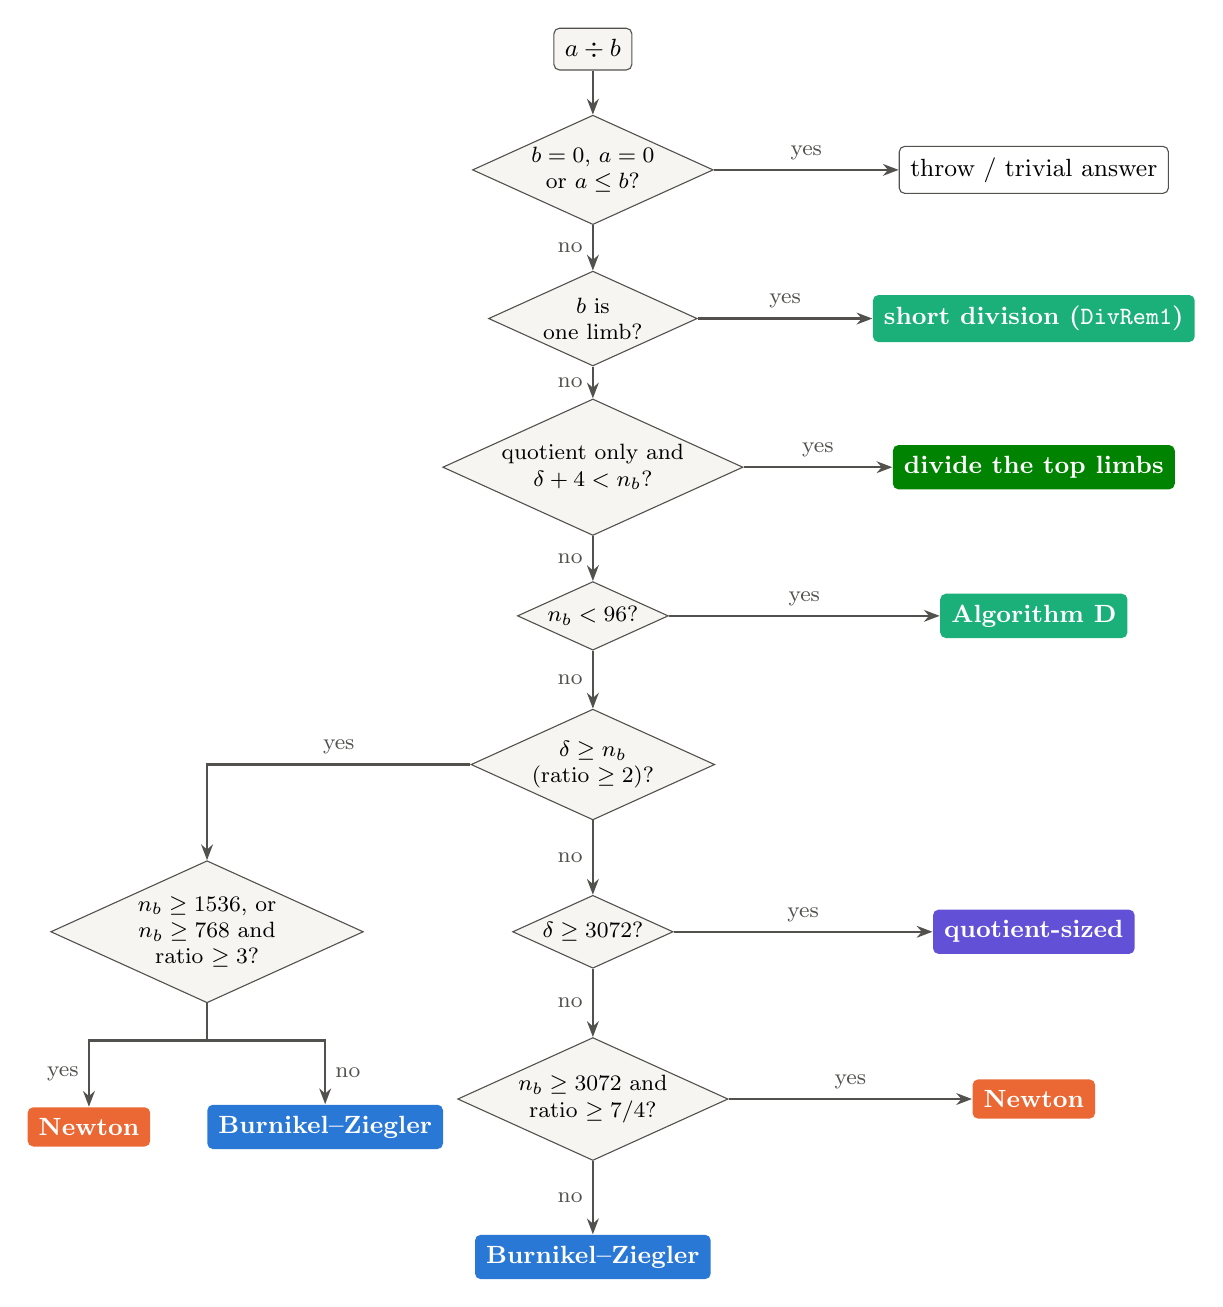
\begin{tikzpicture}[x=1cm,y=1.18cm]
  \node[box,fill=paper] (start) at (0,0) {$a \div b$};
  \node[dec] (triv) at (0,-1.3) {$b = 0$, $a = 0$\\or $a \le b$?};
  \node[box] (trivr) at (5.6,-1.3) {throw / trivial answer};
  \node[dec] (one) at (0,-2.9) {$b$ is\\one limb?};
  \node[algo,fill=sAqua] (sd) at (5.6,-2.9) {short division (\code{DivRem1})};
  \node[dec] (qo) at (0,-4.5) {quotient only and\\$\delta + 4 < n_b$?};
  \node[algo,fill=sGreen] (top) at (5.6,-4.5) {divide the top limbs};
  \node[dec] (small) at (0,-6.1) {$n_b < 96$?};
  \node[algo,fill=sAqua] (kn) at (5.6,-6.1) {Algorithm D};
  \node[dec] (ratio) at (0,-7.7) {$\delta \ge n_b$\\(ratio $\ge 2$)?};
  % ratio >= 2 branch, to the left
  \node[dec] (n2) at (-4.9,-9.5) {$n_b \ge 1536$, or\\$n_b \ge 768$ and\\ratio $\ge 3$?};
  \node[algo,fill=sOrange] (newt1) at (-6.4,-11.6) {Newton};
  \node[algo,fill=sBlue] (bz1) at (-3.4,-11.6) {Burnikel--Ziegler};
  % ratio < 2 branch, downward
  \node[dec] (q1) at (0,-9.5) {$\delta \ge 3072$?};
  \node[algo,fill=sViolet] (qs) at (5.6,-9.5) {quotient-sized};
  \node[dec] (q2) at (0,-11.3) {$n_b \ge 3072$ and\\ratio $\ge 7/4$?};
  \node[algo,fill=sOrange] (newt2) at (5.6,-11.3) {Newton};
  \node[algo,fill=sBlue] (bz2) at (0,-13.0) {Burnikel--Ziegler};
  \draw[arr] (start) -- (triv);
  \draw[arr] (triv) -- node[above,lbl]{yes} (trivr);
  \draw[arr] (triv) -- node[left,lbl]{no} (one);
  \draw[arr] (one) -- node[above,lbl]{yes} (sd);
  \draw[arr] (one) -- node[left,lbl]{no} (qo);
  \draw[arr] (qo) -- node[above,lbl]{yes} (top);
  \draw[arr] (qo) -- node[left,lbl]{no} (small);
  \draw[arr] (small) -- node[above,lbl]{yes} (kn);
  \draw[arr] (small) -- node[left,lbl]{no} (ratio);
  \draw[arr] (ratio.west) -| node[pos=0.25,above,lbl]{yes} (n2.north);
  \draw[arr] (ratio) -- node[left,lbl]{no} (q1);
  \draw[arr] (n2.south) -- ++(0,-0.4) -| node[pos=0.75,left,lbl]{yes} (newt1.north);
  \draw[arr] (n2.south) -- ++(0,-0.4) -| node[pos=0.75,right,lbl]{no} (bz1.north);
  \draw[arr] (q1) -- node[above,lbl]{yes} (qs);
  \draw[arr] (q1) -- node[left,lbl]{no} (q2);
  \draw[arr] (q2) -- node[above,lbl]{yes} (newt2);
  \draw[arr] (q2) -- node[left,lbl]{no} (bz2);
\end{tikzpicture}
\caption{The division dispatcher (64-bit limbs). ``Ratio'' is $n_a / n_b$ and $\delta = n_a - n_b$.
Operands of at most 16 limbs each are handled earlier, on the stack, by the operator layer.}
\label{fig:divdispatch}
\end{figure}

\begin{figure}[ht]
\centering
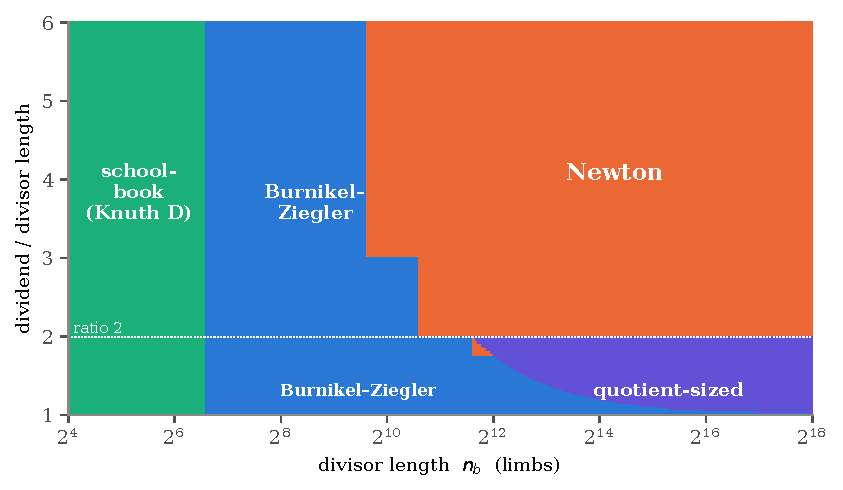
\includegraphics[width=0.88\textwidth]{figures/div_dispatch_map.pdf}
\caption{Which algorithm computes quotient and remainder, by divisor length and length
ratio. Computed from the dispatcher's rules. (Quotient-only calls with ratio below 2 first
shrink the problem to the operands' top limbs, \cref{sec:toplimbs}.)}
\label{fig:divmap}
\end{figure}

\section{The reasoning behind each region}

\paragraph{Divisor under 96 limbs: long division.} Burnikel--Ziegler bottoms out in the same
Algorithm D kernel, so below about 96 limbs the two tie, and the simpler one wins on
overhead. Above it, Burnikel--Ziegler wins at \emph{every} ratio.

\paragraph{Quotient at least as long as the divisor (ratio $\ge 2$).} Here the reciprocal can be
reused across several blocks, so Newton pays off once the divisor is large enough to make
its multiplications NTT-sized: from 1536 limbs, or from 768 limbs when there are at least
three blocks (ratio $\ge 3$) to share the reciprocal's cost. Below that, Burnikel--Ziegler.

\paragraph{Quotient shorter than the divisor (ratio $< 2$).} Now a full reciprocal of the divisor
is wasteful: it is computed to produce a quotient that only the divisor's top limbs
determine. So:
\begin{itemize}
  \item a long quotient ($\ge 3072$ limbs) uses quotient-sized division, Newton on the operands'
        tops plus one back-multiplication;
  \item a large divisor with ratio at least $7/4$ (almost two blocks) still uses Newton;
  \item everything else uses Burnikel--Ziegler, which for a thin quotient already does
        ``divide the tops, multiply back once''.
\end{itemize}

\begin{keyidea}
Long division when the divisor is short; recursive block division in the middle; Newton when
a reciprocal can be reused over several blocks; and when the quotient is short, work only
with the top limbs.
\end{keyidea}

\section{Worked dispatch examples}

\begin{example}[s: which algorithm divides?]
\begin{description}[leftmargin=1.2cm,style=nextline]
  \item[$5000 \div 50$ limbs] Divisor below 96: \textbf{Algorithm D}. Cost about
        $4951 \times 50$ limb steps.
  \item[$2000 \div 1000$] Ratio 2, divisor below 1536, ratio below 3:
        \textbf{Burnikel--Ziegler}.
  \item[$4000 \div 1000$] Ratio 4, divisor $\ge 768$: \textbf{Newton}; one reciprocal shared
        by about three blocks.
  \item[$20\,000 \div 15\,000$, with remainder] $\delta = 5000 \ge 3072$ and smaller than the
        divisor: \textbf{quotient-sized}. Divides the top $\approx 10\,004$ by $5004$ limbs,
        then one $5000 \times 15\,000$ product.
  \item[$10\,500 \div 10\,000$, with remainder] $\delta = 500$, ratio 1.05:
        \textbf{Burnikel--Ziegler}.
  \item[$10\,500 \div 10\,000$, quotient only] $\delta + 4 = 504 < 10\,000$:
        \textbf{top limbs}. Divides the top $1004$ limbs of $a$ by the top $504$ of $b$ (through
        the dispatcher again, which picks Burnikel--Ziegler), and almost never needs the
        confirming product.
  \item[$a \div 7$] One-limb divisor: \textbf{short division}.
\end{description}
\end{example}

\section{How good are the choices?}

The rule was fitted on a grid of divisor lengths from 32 to 262\,144 limbs times
11 ratios from 1.02 to 10, with every algorithm timed directly. Before the re-sweep the
dispatcher was more than 10\% slower than the best algorithm on 69 of 232 grid cells (up to
2.8 times); after it, 3 cells (all under 16\%).

Dispatcher time relative to GMP 6.3, geometric mean over the 11 ratios (single run, M1 Max):

\begin{center}
\small
\begin{tabular}{rcc}
\toprule
divisor limbs & before the 2026-11 re-sweep & after \\
\midrule
32--96 & 1.24--1.27$\times$ & 1.24--1.26$\times$ \\
384 & 1.83$\times$ & 1.35$\times$ \\
768 & 2.19$\times$ & 1.37$\times$ \\
2048 & 1.11$\times$ & 1.08$\times$ \\
4096 & 0.90$\times$ & 0.85$\times$ \\
12288 & 0.61$\times$ & 0.55$\times$ \\
32768 & 0.69$\times$ & 0.61$\times$ \\
\bottomrule
\end{tabular}
\end{center}

Below about 2000 limbs GMP's hand-written assembly is still 1.25--1.4 times faster; from about
4000 limbs BigMath's threaded NTT puts it ahead.

\begin{practice}
\begin{itemize}
  \item Use \code{a / b} when you only need the quotient. For a quotient shorter than the
        divisor it can be dozens of times faster than \code{DivideAndRemainder}, because only the
        top limbs are divided.
  \item Use \code{DivideAndRemainder(a, b)} when you need both: one division gives both, which is
        cheaper than \code{a / b} followed by \code{a \% b}.
  \item Use \code{CachedDivision} when the divisor repeats.
\end{itemize}
\end{practice}

\chapter{Radices and decimal arithmetic}
\label{ch:conv}

Numbers are stored in base $2^{64}$ but read and written in base 10. Because 10 is not a power
of two, converting is real arithmetic: every output digit depends on every input limb. Done
the obvious way it costs $n^2$; BigMath does it with a divide-and-conquer scheme that costs
a logarithmic factor more than one multiplication. The code is in \file{src/common/Parser.cpp}.

\section{Why the obvious method is slow}

The schoolbook way to parse is ``for each digit: $r \leftarrow 10r + \text{digit}$''. With $L$
digits that is $L$ big-number operations, each on a number of up to $L/19$ limbs: about
$L^2/19$ limb operations. Printing the schoolbook way (``divide by 10, emit the remainder'') is
equally quadratic. At a million digits that is around $10^{10}$ operations.

The library removes this cost in two layers: a constant-factor speedup (handle 18--19 digits
at a time) and an asymptotic one (divide and conquer).

\section{Small numbers: 18 or 19 digits at a time}
\label{sec:linparse}

\textbf{Parsing.} Instead of one digit, take 18 at a time: $10^{18} < 2^{63}$, so 18 digits fit in
one limb with headroom. Each step is $r \leftarrow r \cdot 10^{18} + \text{chunk}$: one
multiply-by-one-limb and one add over the current value. That is 18 times fewer big-number
operations than digit by digit.

\begin{example}[: parsing a 25-digit number]
\code{"1234567890123456789012345"} has 25 digits. $25 = 7 + 18$, so the first chunk is the
leading 7 digits and then one full 18-digit chunk:
\begin{align*}
r &= 1\,234\,567\\
r &= 1\,234\,567 \cdot 10^{18} + 890\,123\,456\,789\,012\,345 .
\end{align*}
Two steps instead of 25.
\end{example}

\textbf{Printing.} Divide by $10^{19}$ (the largest power of ten that fits in a limb) repeatedly;
each remainder is a block of 19 digits. Each division is the fast single-limb division of
\cref{sec:shortdiv}.

\begin{example}[: printing $2^{64}$]
$2^{64}$ is the limbs $[0, 1]$. Dividing by $10^{19}$ gives quotient $1$ and remainder
$8\,446\,744\,073\,709\,551\,616$. The quotient is printed without padding and the remainder is
padded to 19 digits: \code{"1" + "8446744073709551616"} $= 18\,446\,744\,073\,709\,551\,616$.
\end{example}

These ``linear'' routines are still quadratic overall, but with a small constant. They handle
numbers up to 2048 digits for parsing (\code{BIGMATH\_PARSE\_DC\_THRESHOLD}) and below 1024
digits for printing (\code{BIGMATH\_TOSTR\_DC\_THRESHOLD}), and the leaves of the
divide-and-conquer recursion below.

\section{Large numbers: divide and conquer}

\subsection{Parsing}

Split the digit string in the middle. Parse each half (recursively), then combine:
\[
\text{value} = \text{high} \times 10^{\,\text{digits in low half}} + \text{low} .
\]
Each level costs one big multiplication of about half the total size, and the recursion has
$\log_2 L$ levels: $T(L) = 2\,T(L/2) + \M(L)$, about $\M(L)\log L$ in total.

\begin{figure}[ht]
\centering
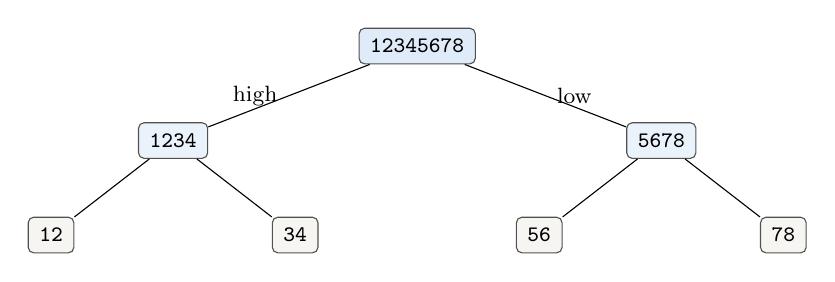
\begin{tikzpicture}[level distance=12mm,
  level 1/.style={sibling distance=62mm},
  level 2/.style={sibling distance=31mm},
  every node/.style={box,font=\footnotesize\ttfamily}]
  \node[fill=sBlue!15] {12345678}
    child {node[fill=sBlue!10] {1234}
      child {node[fill=paper] {12}}
      child {node[fill=paper] {34}}
      edge from parent node[draw=none,fill=none,left,font=\footnotesize\rmfamily] {high}}
    child {node[fill=sBlue!10] {5678}
      child {node[fill=paper] {56}}
      child {node[fill=paper] {78}}
      edge from parent node[draw=none,fill=none,right,font=\footnotesize\rmfamily] {low}};
\end{tikzpicture}

\smallskip
{\small Parse upward: $12 \cdot 10^2 + 34 = 1234$, \ $56\cdot 10^2 + 78 = 5678$, \
$1234 \cdot 10^4 + 5678 = 12\,345\,678$.}
\caption{Divide-and-conquer parsing. Leaves use the 18-digit method; each join is one
multiplication by a power of ten.}
\end{figure}

The powers of ten come from \code{Pow10}, which caches them per thread and builds even powers
by \emph{squaring} ($10^{2k} = (10^k)^2$, using the faster square path). After the first
conversion of a given size, the powers are free.

\subsection{Printing}

Printing is the same tree read downward: divide by $10^{k}$, where $k$ is half the digit count.
The quotient gives the top half of the digits, the remainder the bottom half. Recurse on both.

\begin{figure}[ht]
\centering
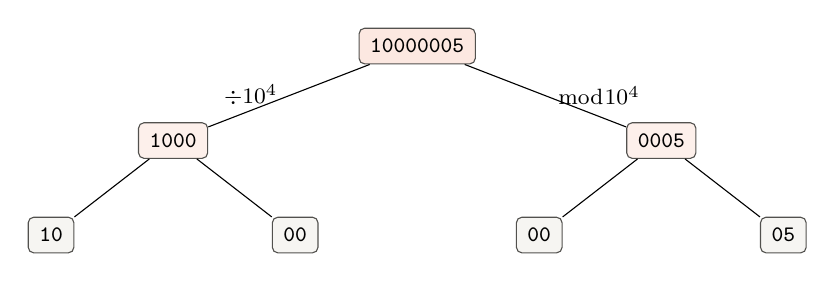
\begin{tikzpicture}[level distance=12mm,
  level 1/.style={sibling distance=62mm},
  level 2/.style={sibling distance=31mm},
  every node/.style={box,font=\footnotesize\ttfamily}]
  \node[fill=sOrange!15] {10000005}
    child {node[fill=sOrange!10] {1000}
      child {node[fill=paper] {10}}
      child {node[fill=paper] {00}}
      edge from parent node[draw=none,fill=none,left,font=\footnotesize\rmfamily] {$\div 10^4$}}
    child {node[fill=sOrange!10] {0005}
      child {node[fill=paper] {00}}
      child {node[fill=paper] {05}}
      edge from parent node[draw=none,fill=none,right,font=\footnotesize\rmfamily] {$\bmod 10^4$}};
\end{tikzpicture}
\caption{Divide-and-conquer printing of $10\,000\,005$. The remainder $5$ must be written as
\code{0005}: every lower half is padded with zeros to its full width. Only the very top
piece is printed without leading zeros.}
\end{figure}

The divisions are by the same few powers of ten again and again, which is exactly the case
for cached reciprocals (\cref{sec:cached}). For each level of the tree the library stores a
\emph{divider}: the power $10^{k}$ and its Newton reciprocal. The chain of dividers is cached
per thread and reused by later conversions of similar size: the chain's top size is rounded
up to a grid of 16 steps per doubling, so numbers of slightly different lengths share one
chain.

\begin{perfnote}
Before the cached dividers existed, every division in the tree rebuilt its reciprocal, and the
divide-and-conquer printer was \emph{slower} than the quadratic one; it had been tried and
reverted. With cached reciprocals, printing a 100\,000-digit number went from 383\,ms to
45.5\,ms; caching whole divider chains across calls halved warm times again. For small tree
levels (below 13\,000 digits single-threaded, 6\,500 with threads) a cached Newton reciprocal
does not pay, and those levels use the ordinary division dispatcher instead.
\end{perfnote}

\begin{pitfall}
An early version split by $10^{18}, 10^{36}, 10^{72}, \dots$, powers of two times 18 digits,
hoping fewer distinct divisors would help. The splits came out lopsided: a 500\,000-digit
number split into 363\,000 and 137\,000 digits instead of two halves. The recursion lost its
balance and became slower than the quadratic printer (1899\,ms against 1700\,ms). Splits must
be close to the middle; the current rounding keeps them within 56/44.
\end{pitfall}

\subsection{Using several cores}

From 100\,000 digits (\code{BIGMATH\_PARSE\_PARALLEL\_THRESHOLD},
\code{BIGMATH\_TOSTR\_PARALLEL\_THRESHOLD}), both directions descend three levels of the tree on
the calling thread, then hand the $2^3 = 8$ independent subtrees to the thread pool in one
batch. Each worker converts its subtree serially. The calling thread then does the remaining
joins (parsing) or assembles the string (printing). Because every lower half has a known,
fixed width, each subtree can write straight into its slot of the output string.

\section{Cost in practice}

\begin{center}
\small
\begin{tabular}{lrrr}
\toprule
operation & BigMath, 1 thread & GMP, 1 thread & default build $\div$ GMP \\
\midrule
parse 100\,000 digits & 1.644\,ms & 1.057\,ms & 0.52$\times$ \\
parse 20\,000\,000 digits & 910.3\,ms & 809.8\,ms & 0.21$\times$ \\
print 100\,000 digits & 3.186\,ms & 2.382\,ms & 0.52$\times$ \\
print 20\,000\,000 digits & 2\,546\,ms & 2\,118\,ms & 0.24$\times$ \\
\bottomrule
\end{tabular}

\smallskip
{\footnotesize Median warm times from three fresh processes on the M1 Max, revision \code{7b3cc04}. The last column is
time of the default build (up to eight threads) divided by single-thread GMP time.}
\end{center}

\begin{practice}
\begin{itemize}
  \item The first conversion at a new size builds powers of ten and dividers; later ones reuse
        them. Benchmark the second call, and expect the first to be slower.
  \item Workers share immutable CRT transform tables. Each thread reuses writable buffers
        across linear and cyclic products. For full fused matrix products, decimal conversion
        processes the three primes in sequence from length $2^{20}$, using two scratch
        buffers. Standalone multiplication uses this schedule from $2^{24}$.
  \item If no human needs to read the number (storage, hashing, sending it to another
        program), use its limbs directly (\code{x.Limbs()}): that needs no conversion at all.
\end{itemize}
\end{practice}

\newpage
\section{Converting digit vectors between radices}
\label{sec:convertbase}

\code{ConvertBase} takes a little-endian vector of digits or an inclusive
index range within that vector. An equal-radix conversion copies the selected
digits as stored. When the two radices are distinct powers of two, the digits
describe the same bit sequence in different group widths. The implementation
treats \code{Base2\_64}, the radix sentinel with value zero, as a 64-bit width.

The repacker appends each source digit to a 128-bit buffer, starting at the low
end. It emits a target digit whenever enough bits are available, taking the
low bits and shifting them out of the buffer. At most 63 bits are left before
the next source digit arrives. The repacker emits any final partial digit and
trims high zero digits. An empty or all-zero input repacks to \code{\{0\}}.
The work is linear in the combined input and output digit counts.

\begin{example}
In base $2^{31}$, the little-endian pair \code{[0x12345678, 3]} represents
$3\cdot 2^{31} + \texttt{0x12345678}$. In base $2^{16}$ the digits are
\code{[0x5678, 0x9234, 1]}. The high bit of the middle target digit
comes from the low bit of the second source digit.
\end{example}

The remaining radix changes use Horner's rule. Read source digits
from high to low, multiplying the accumulated result by the source radix and
adding the next digit. For a $2^{64}$ source, one step shifts each target digit
left by 64 in a 128-bit word, adds the carry (initially the next source limb),
and divides by the target radix. The remainder replaces the target digit and
the quotient becomes the next carry. See \file{src/algorithms/BaseConversion.cpp}.
Decimal strings use the parsing and formatting routines described above.

\section{Fixed-point decimal arithmetic}
\label{sec:bigdecimal}

A \code{BigDecimal} represents $u\cdot 10^{-s}$, where $u$ is a signed
\code{BigInteger} and $s$ is an integer scale. For example,
\code{12.340} has $u=12340$ and $s=3$. A negative scale represents
trailing integer zeros. Addition and subtraction align scales, and
multiplication multiplies the unscaled integers and adds their scales.
These operations are exact.

\code{a.Divide(b, scale, mode)} returns a value at the requested scale.
If the operands have scales $s_a,s_b$ and the requested scale is $t$,
scale the integer numerator or denominator so the unscaled quotient
represents $(u_a/u_b)\,10^{t+s_b-s_a}$. The integer division produces a
quotient magnitude $q$ and a remainder $r$. For rounding to nearest,
compare $2r$ with the positive divisor. On a tie, \code{HALF\_UP} increases
the magnitude, \code{HALF\_DOWN} leaves it, and \code{HALF\_EVEN} selects
the even result. \code{UP} moves away from zero, \code{DOWN} truncates
toward zero, and \code{CEILING} and \code{FLOOR} round toward the
respective infinities. \code{UNNECESSARY} requires a zero remainder.

\begin{example}
At scale 5, dividing the scaled numerator by 3 gives $100000=3\cdot33333+1$.
\code{BigDecimal("1").Divide(BigDecimal("3"), 5, RoundingMode::HALF\_EVEN)}
returns \code{0.33333}. With \code{UP} it returns \code{0.33334}.
With \code{UNNECESSARY} it throws. A repeating decimal such as $1/3$
is rounded to a finite value at every requested scale.
\end{example}

\code{SetScale} uses the same rounding rules when reducing the scale.
\code{CompareTo} compares numeric values. \code{Equals} also requires
the scales to match, so \code{1.20} and \code{1.2} compare as the same
value while preserving their distinct scales.

\chapter{Number theory and integer roots}
\label{ch:numbertheory}

Include \file{biginteger/ops/NumberTheory.h} or \file{biginteger/ops/Operations.h}
for the APIs in this chapter. The prime tests give exact answers below
$2^{64}$ and probabilistic answers above that range.

\section{Greatest common divisors and B\'ezout coefficients}
\label{sec:gcd}

\code{Gcd(a, b)} returns the nonnegative greatest common divisor of signed inputs.
\code{ExtendedGcd(a, b)} also returns coefficients $x$ and $y$ satisfying
$a x + b y = \gcd(a,b)$. Both functions accept zero. For two zero inputs, the
divisor and both coefficients are zero.

One Euclidean step replaces $(a,b)$ by $(b,a-qb)$, where $q$ is the quotient
of $a$ divided by $b$. The common divisors stay the same. Extended GCD applies
the same step to the coefficients of the two remainders, so they remain linear
combinations of the original inputs.

\begin{example}
$240=5\cdot46+10$, then $46=4\cdot10+6$, $10=6+4$, and
$6=4+2$. Substituting back gives $2=-9\cdot240+47\cdot46$.
The coefficient pair need only satisfy the identity.
\end{example}

BigMath uses Lehmer's algorithm to batch steps when both remainders have
the same limb count and have at least two limbs. It predicts quotients from
a common leading prefix of at most 62 bits and bounds what the omitted
low limbs could contribute. A batch is used only when those bounds certify
at least two steps. A two-by-two matrix applies the batch to the full
remainders and, for extended GCD, to the coefficient pairs. An exact
division step handles cases where a batch cannot be certified. Plain GCD
finishes with a scalar remainder and a single-limb GCD when the second
operand fits in one limb.

\subsection{Recursive half-GCD}
\label{sec:halfgcd}

For large inputs, BigMath uses \href{https://doi.org/10.1090/S0025-5718-07-02017-0}{M\"oller's difference-based half-GCD}.
Subtracting $q$ times one entry from the other is a determinant-one
matrix operation. It has an integer inverse, so the two entries keep
the same common divisors. A product of these matrices represents a
whole reduction and can also act on the B\'ezout coefficients.

With $N$ the larger bit length, the recursive step works on the leading
bits and applies the resulting matrix to the full operands. For two
entries wider than $s=\floor{N/2}+1$ bits, it preserves that lower bound
and reduces their absolute difference to at most $s$ bits. The difference
test and exact correction steps control the effect of the omitted low
bits. Below or at 2\,048 bits, the recursion uses bounded Lehmer batches
and exact steps.

The shorter operand must have at least 65\,536 bits for \code{Gcd} or
16\,384 bits for \code{ExtendedGcd}, and its bit length must exceed
$\floor{N/2}+1$. A wider imbalance falls through to exact division.
Plain GCD applies one high-half reduction at a time. Extended GCD
composes a larger transform and applies it to both coefficient pairs.
The recursive algorithm costs $\bigO(\M(N)\log N)$, with $\M(N)$ the
cost of multiplying $N$-bit integers.

\begin{perfnote}
For balanced 262\,144-bit operands, paired single-threaded tests on
the M1 Max measured 2.93$\times$ faster GCD and 4.58$\times$ faster
extended GCD versus the Lehmer-based implementation.
\href{https://github.com/mmurshed/biginteger/blob/main/BENCHMARK.md\#recursive-half-gcd}{Measurement details}
\end{perfnote}

\section{Integer square root with a remainder}
\label{sec:sqrtrem}

\code{SqrtRem(n)} returns $(s,r)$ such that
$s=\floor{\sqrt n}$, $n=s^2+r$, and $0\le r\le 2s$.
It accepts zero and throws for negative inputs. For example, \code{SqrtRem(80)}
gives $(8,16)$ because $80=8^2+16$ and $9^2=81$.

For one or two limbs, a floating-point estimate supplies a starting root.
The code checks it with integer arithmetic and corrects it by integer Newton
iteration when necessary. Inputs too small for a recursive split likewise
use Newton iteration, seeded from leading bits.

For larger inputs, BigMath uses Zimmermann's divide-and-conquer square root.
Choose a limb-aligned radix $D$ and write $n=aD^2+bD+c$. Recursively compute
$h=\floor{\sqrt a}$ and $r_h=a-h^2$. Divide $r_h D+b$ by $2h$ to get a quotient
$q$ and remainder $t$. Expanding the trial root $hD+q$ gives
\[
n-(hD+q)^2=tD+c-q^2 .
\]
The split keeps $h\ge D/2$, so if the trial remainder is negative, one
decrement of the trial root suffices. To update the remainder after the
decrement, add twice the trial root minus one.

\begin{example}[ with radix 10]
For $n=2759$, the blocks are $27$, $5$, and $9$. The high root is $5$ with
remainder $2$. Dividing $25$ by $10$ gives $q=2$ and $t=5$, so the
root is $52$ and the remainder is $50+9-4=55$.
\end{example}

\newpage
\section{Integer roots of other degrees}
\label{sec:nthroot}

\code{RootRem(n, degree)} returns $(x,r)$ with $r=n-x^e$ for degree
$e$. The root is rounded toward zero. Negative inputs require an odd
degree. For a nonnegative input, $x^e\le n<(x+1)^e$. Degree zero throws,
degree one returns the input with remainder zero, and degree two uses
\code{SqrtRem}.

\begin{example}
\code{RootRem(-80, 3)} returns $(-4,-16)$ since $(-4)^3=-64$ and
$(-5)^3=-125$.
\end{example}

Magnitudes that fit in 64 bits use native binary search for other
degrees. A nonzero magnitude has root one if the degree is at least
its bit length. For the other inputs, BigMath first finds an exact leading
prefix of the root by binary search. To find the prefix with $s$ low
root bits removed, take the integer $e$th root of
$\floor{|n|/2^{es}}$. A prefix $p$ then bounds the full root from
above by $(p+1)2^s$.

BigMath refines the prefix in stages of increasing precision. Each
stage starts just above the root for its truncated input $A$ and
uses the integer Newton step
\[
  x_{\mathrm{next}} =
  \floor{\frac{(e-1)x+\floor{A/x^{e-1}}}{e}} .
\]
The first step that would stay at $x$ or increase it signals that
$x$ is the integer root for that stage. Exponentiation stops early
when a trial power exceeds $A$. The final stage uses the full input
and forms the remainder from the final power.

\begin{perfnote}
On the M1 Max, the sampled 64-bit \code{RootRem} call at degree three
took 0.094\,\textmu s in BigMath and 0.106\,\textmu s in GMP. At
262\,144 bits, it took 1.55\,ms in BigMath and 0.75\,ms in GMP.
\href{https://github.com/mmurshed/biginteger/blob/main/BENCHMARK.md\#integer-nth-root-and-remainder}{Measurements and degree sweep}
\end{perfnote}

\newpage
\section{Modular powers}
\label{sec:powmod}

\code{PowMod(a, e, m)} returns $a^e\bmod m$ in $[0,m)$.
The base may be signed, the exponent must be nonnegative, and the
modulus must be positive. An exponent of zero returns $1\bmod m$,
which is zero when $m=1$.

Repeated squaring processes the binary digits of $e$ and reduces each
intermediate product modulo $m$. For a dense exponent, a sliding window
uses a table of odd powers to handle several bits at once. Sparse or short
exponents use the binary path. In $7^{13}\bmod 11$, the powers for
exponents $1,4,8$ have residues $7,3,9$ and their product has residue $2$.

\begin{itemize}
  \item A single-limb modulus uses machine-word arithmetic.
  \item An odd modulus of at least 64 limbs and an exponent of at least
        64 bits use FastREDC by default. Otherwise, odd multi-limb moduli
        through 128 limbs use limb-by-limb Montgomery reduction for
        exponents of at least 16 bits.
  \item An even modulus of at most 128 limbs with a power-of-two factor
        $2^k$, where $0<k<\log_2 B$, can use the Chinese remainder
        theorem for exponents of at least 16 bits. The implementation
        splits off $2^k$ and applies the usual dispatch to the odd part.
  \item Other cases use the usual multiplication and division dispatchers.
\end{itemize}

The runtime depends on the operands and the exponent's bits.

\subsection{Montgomery reduction and FastREDC}
\label{sec:fastredc}

For an odd $n$-limb modulus $m$, let $R=B^n$. Montgomery form represents
$x$ by $xR\bmod m$. Multiplying two encoded residues gives $T<m^2$.
Computing $T/R\bmod m$ restores the encoding. Let $m'=-m^{-1}\bmod R$.
Then
\[
q=(T m')\bmod R, \qquad u=\frac{T+qm}{R}.
\]
The low $n$ limbs of $T+qm$ cancel. Dropping them gives $u<2m$, so one
conditional subtraction puts the result in $[0,m)$.

The base case cancels one limb at a time. FastREDC doubles the known
width of the inverse to precompute $m'$ once and uses a low product for
$q$. The initial product or square goes through BigMath's usual
dispatcher. With CRT enabled, reductions from 512 limbs can recover
the high part of $qm$ from a cyclic product. Write $qm=\ell+RH$, where
$\ell=(-T)\bmod R$ is already known. If $W=qm\bmod(B^L-1)$, subtract
$\ell$ and multiply by $B^{L-n}$ modulo $B^L-1$, a limb rotation, to recover $H$.
The bound $H<m$ makes that recovery unique. The cyclic path rounds $L$
up to a power of two within the standard CRT transform limit.

\begin{perfnote}
In paired single-threaded M1 Max runs, FastREDC sped up dense
8\,192-bit powering by 1.23$\times$. A 65\,536-bit modulus with a
257-bit exponent sped up by 1.57$\times$. These ratios include setup.
\href{https://github.com/mmurshed/biginteger/blob/main/BENCHMARK.md\#subquadratic-montgomery-reduction}{Measurement details}
\end{perfnote}

\newpage
\section{Primality testing and finding the next prime}
\label{sec:prime}

\code{IsProbablePrime(n, rounds)} rejects values below 2 and screens small
factors before running Miller--Rabin. The test writes $n-1=2^s d$ with $d$
odd. For a witness base $a$, it computes $a^d\bmod n$ and squares the residue
up to $s-1$ times. The first value may be $1$ or $-1$ modulo $n$. Otherwise,
one of the later squares must reach $-1$ for the witness to pass.

The deterministic word path uses three fixed bases through 32 bits and
seven through the rest of the unsigned 64-bit range. For larger values it
screens base 2, then samples uniformly from $[2,n-2]$ by rejection.
With $k$ independent uniform random witnesses, the chance that any
fixed odd composite passes all $k$ is at most $4^{-k}$. The default is
32 random witnesses. Both prime APIs require a positive round count.
Miller--Rabin uses the FastREDC cutoff with $d$ as the exponent and
reuses the precomputed inverse across witnesses in the same test.
The default build can test witnesses in parallel when the candidate
has at least 1,024 bits and at most 128 limbs and the caller requests
at least eight random rounds. Wider candidates can use the pool inside
individual products.

\code{NextProbablePrime(n, rounds)} searches strictly above $n$ and returns
2 for $n<2$. For example, a search starting at 29 returns 31. For
word-size starting values it tests odd candidates directly. For larger
starting values, it marks multiples of small odd primes in segments of
1,024 odd candidates. Each small prime's next offset carries forward to the
next segment. The sieve uses primes below 4,096 through 512 bits and below
32,768 above that size.

The first sieve survivor is tested on its own. In the parallel size range
(at least 1,024 bits and at most 128 limbs), the search can then screen
up to eight survivors at a time with base 2. It applies the randomized
tests to the passing candidates in ascending order, so completion order
cannot select a later result.

\begin{practice}
\file{BENCHMARK.md} records separate GMP comparisons for these operations,
including dense and sparse exponents and ordinary and long prime gaps.
In a Release build with GMP available, build \code{number\_theory\_vs\_gmp}.
Use \code{gcd-large} for recursive GCD or \code{powmod-large} for FastREDC.
The \code{gcd}, \code{sqrtrem}, \code{powmod}, \code{prime}, and
\code{nextprime} modes isolate the other measurements.
\end{practice}

\newpage
\section{Factorials and binomial coefficients}
\label{sec:combinatorics}

\code{Factorial(n)} computes $n!$, including $0!=1$. A native table covers
$0$ through $20$. For larger inputs, a product tree packs consecutive
factors into limbs and multiplies the packed groups in balanced pairs.
The tree gives the multiplication dispatcher similarly sized operands.

\subsection{Prime swing}

Prime swing starts at $n=512$ with 64-bit limbs and at $64$ with
32-bit limbs. Let $O(n)$ be the odd part of $n!$. The recursion uses
\[
  O(n)=O(\floor{n/2})^2
  \prod_{\substack{p\le n\\p\ \mathrm{odd\ prime}}}
       p^{\,\sum_{j\ge1}(\floor{n/p^j}\bmod 2)}.
\]
For each odd prime, the exponent counts the powers $p^j$ for which
$\floor{n/p^j}$ is odd. BigMath sieves once up to $n$ and reuses
prefixes of the prime list at smaller recursive sizes. The product
tree combines the swing factors. A final shift restores the
$n-\operatorname{popcount}(n)$ factors of two.

\begin{example}
For $10!$, the odd part of $5!$ is $15$ and the swing is $3^2\cdot7$.
Thus $O(10)=15^2\cdot63=14\,175$. Shifting by eight bits gives
$10!=3\,628\,800$.
\end{example}

\subsection{Binomial coefficients by exact division or prime powers}

\code{Binomial(n, k)} returns zero for $k>n$ and otherwise replaces $k$
by $\min(k,n-k)$. Through 32 terms, it packs batches of numerator
and denominator factors into limbs. Each batch ends at a binomial
coefficient, so \code{DivideExact} can divide the accumulated product
(\cref{sec:exactdivision}). Wider off-center cases build two packed
product trees and divide once.

For $n\ge512$ and reduced $k\ge\floor{n/8}$, the central path builds
the answer from prime powers. The exponent of $p$ is
$v_p(n!)-v_p(k!)-v_p((n-k)!)$, where
$v_p(j!)=\sum_{i\ge1}\floor{j/p^i}$. This path reuses the factorial
sieve and packed product tree, then restores the power of two.

\begin{perfnote}
On the M1 Max, the default 64-bit build took 28.01\,ms for
$1\,000\,000!$ and 5.61\,ms for $\binom{1\,000\,000}{500\,000}$.
GMP took 78.47\,ms and 5.91\,ms on those fixtures.
Use \code{number\_theory\_vs\_gmp factorial} or
\code{number\_theory\_vs\_gmp binomial} to reproduce the comparisons.
\end{perfnote}

\newpage
\section{Chinese remaindering with a reusable product tree}
\label{sec:crtplan}

\code{ChineseRemainderPlan} takes a nonempty list of pairwise coprime
word moduli $m_i\ge2$ and owns its precomputed data. Write
$M=\prod_i m_i$. \code{Reduce(value)} returns the least nonnegative
residue for each modulus in input order, including when the input is
negative. \code{Reconstruct(residues)} returns the unique integer in
$[0,M)$ with those residues.

\subsection{What the plan precomputes}

The plan packs consecutive moduli into groups whose products fit in
one word. A tree stores the product of each pair of child groups or
subtrees. The root holds $M$. A pass down the tree computes
$c_i=M/m_i\bmod m_i$ and precomputes its inverse $t_i$ modulo $m_i$.
If any inverse is missing, the moduli share a factor and construction
throws.

\subsection{Downward remainders and upward reconstruction}

For reduction, pass the input remainder down the tree, taking it
modulo each child's product. At a leaf, a word reduction supplies the
residue for the group. Each group then reduces to its individual
moduli. For reconstruction with residues $r_i$, the weighted terms
are
\[
  S=\sum_i \bigl(r_i t_i\bmod m_i\bigr)\frac{M}{m_i}.
\]
Modulo $m_i$, every term except the $i$th vanishes. At a tree node,
the implementation scales each child's contribution by the other
child's product and adds them. Leaves use word arithmetic and the
root reduces the result modulo $M$.

\begin{example}
With moduli $(3,5,7)$ and residues $(2,3,2)$, the cofactors are
$(35,21,15)$ and their inverses are $(2,1,1)$ in the respective
moduli. The weighted sum is $35+63+30=128$, so the representative
modulo $105$ is $23$.
\end{example}

\begin{practice}
Reuse one plan for repeated calls with the same moduli. The benchmark
times setup separately. For 8\,192 moduli of 61 bits on the M1 Max,
reconstruction took 3.17\,ms in the default 64-bit build and
3.77\,ms in FLINT. FLINT was faster at the smaller sampled sizes.
\href{https://github.com/mmurshed/biginteger/blob/main/BENCHMARK.md\#product-tree-chinese-remaindering}{Setup, reduction, and reconstruction timings}
\end{practice}

\newpage
\section{Bounded rational reconstruction}
\label{sec:rationalreconstruction}

\code{ReconstructRational(a, m, N, D)} looks for a reduced fraction
$n/d$ with $|n|\le N$, $0<d\le D$, and $n\equiv ad\pmod m$.
It accepts signed residues and normalizes them to $[0,m)$. An empty
optional means there is no fraction within the bounds. The call
requires $m>1$, $N\ge0$, $D>0$, and $2ND<m$.

The strict bound makes the fraction unique. If two candidates share
the residue, $m$ divides $n_1d_2-n_2d_1$. Its absolute value is at
most $2ND$, so it must be zero. The positive denominator and
reduced form fix both signs and the common scale.

Extended Euclid starts with $m$ and $a$ and tracks the coefficient of
$a$ in each remainder. It stops at the first remainder at most $N$.
That remainder and its coefficient give the numerator and denominator
after sign normalization. BigMath checks the denominator bound and
that the two are coprime. It uses Lehmer batches and recursive half-GCD
only while both remainders stay above the stopping bound
(\cref{sec:halfgcd}).

\begin{example}[ after Chinese remaindering]
The residues $(3,1,2)$ modulo $(5,7,11)$ give $a=288$ modulo $385$.
With $N=D=5$, the successive remainders are $97$, $94$, and $3$.
The coefficient of $288$ at remainder $3$ is $-4$, since
$3=3\cdot385-4\cdot288$. The normalized fraction is $-3/4$.
\end{example}

\begin{perfnote}
On the M1 Max, half-GCD reduced the two sampled 262\,144-bit
reconstructions from 77--119\,ms to about 21\,ms. FLINT took
11--14\,ms. With FLINT and GMP available, the
\code{rational\_reconstruction\_vs\_flint} target reproduces the comparison.
\href{https://github.com/mmurshed/biginteger/blob/main/BENCHMARK.md\#bounded-rational-reconstruction}{Measurements and test fixtures}
\end{perfnote}

\chapter{Threads: the internal pool}
\label{ch:parallel}

By default BigMath runs a small pool of worker threads and uses it \emph{inside} single
operations: one large multiplication is spread over several cores. You do not have to do
anything to use it, and you can switch it off at build time
(\code{-DBIGMATH\_USE\_THREADS=0}). The code is in \file{src/common/Parallel.cpp}.

\section{What runs in parallel}

\begin{center}
\small
\begin{tabularx}{\textwidth}{lX}
\toprule
operation & how the work is split \\
\midrule
addition / subtraction & if enabled by the profile, equal-length magnitudes use blocks
                         with a carry or borrow fixup (\cref{sec:paralleladdsub}) \\
NTT product & Ordinary CRT batches operand--prime transforms. The fused matrix method
              schedules transpose tiles across the pool at each stage. Finalization
              splits the carries into ranges (\cref{sec:nttthreads}). \\
parse / print $\ge$ 100\,000 digits & 8 independent subtrees of the divide-and-conquer tree \\
division, conversion & indirectly: their large products are NTT products \\
Miller--Rabin & independent randomized witnesses once base 2 passes \\
next probable prime & base-2 screens of sieve survivors, then randomized tests in
                      candidate order (\cref{sec:prime}) \\
\bottomrule
\end{tabularx}
\end{center}

Small operations never touch the pool. Schoolbook, Karatsuba, Toom-3 and long division are
single-threaded: at their sizes, handing work to another core costs more than doing it.

\section{Size of the pool}

The pool has $\min(\text{hardware threads}, 8)$ threads (\code{BIGMATH\_MAX\_THREADS}),
counting the calling thread, which always does a share of the work itself. Eight is a
deliberate cap: on the M1 Max more threads competed for the shared L2 cache during NTTs and
did not help.

\section{Warm and cold}
\label{sec:warmcold}

A worker that has nothing to do spins for 100\,\textmu s (\code{BIGMATH\_POOL\_SPIN\_US}) waiting for
new work, then goes to sleep. Waking a sleeping thread takes the operating system 20--30\,\textmu s.
For a large product that is nothing. For a mid-sized NTT product, which takes about 25\,\textmu s
with all cores working, it is as long as the whole job.

\begin{figure}[ht]
\centering
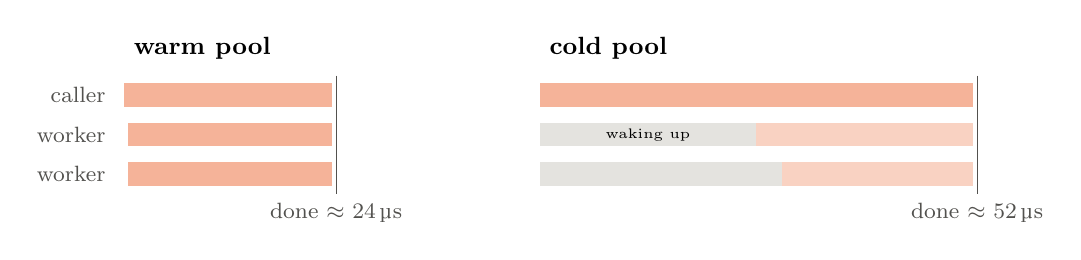
\begin{tikzpicture}[x=0.11cm,y=0.5cm]
  \node[lbl,anchor=east] at (-1,0) {caller};
  \node[lbl,anchor=east] at (-1,-1) {worker};
  \node[lbl,anchor=east] at (-1,-2) {worker};
  \node[font=\small\bfseries,anchor=west] at (0,1.2) {warm pool};
  \fill[sOrange!50] (0,-0.3) rectangle (24,0.3);
  \fill[sOrange!50] (0.5,-1.3) rectangle (24,-0.7);
  \fill[sOrange!50] (0.5,-2.3) rectangle (24,-1.7);
  \draw[ink2] (24.5,0.5) -- (24.5,-2.5) node[below,lbl] {done $\approx$ 24\,\textmu s};
  \begin{scope}[shift={(48,0)}]
    \node[font=\small\bfseries,anchor=west] at (0,1.2) {cold pool};
    \fill[sOrange!50] (0,-0.3) rectangle (50,0.3);
    \fill[rule] (0,-1.3) rectangle (25,-0.7); \node[font=\tiny] at (12.5,-1) {waking up};
    \fill[sOrange!30] (25,-1.3) rectangle (50,-0.7);
    \fill[rule] (0,-2.3) rectangle (28,-1.7);
    \fill[sOrange!30] (28,-2.3) rectangle (50,-1.7);
    \draw[ink2] (50.5,0.5) -- (50.5,-2.5) node[below,lbl] {done $\approx$ 52\,\textmu s};
  \end{scope}
\end{tikzpicture}
\caption{A small NTT product with a warm and with a cold pool (schematic). Cold, the caller
does most of the work alone while the workers wake up, so the product costs about its
single-threaded time.}
\end{figure}

This is why the multiplication dispatcher checks the pool's temperature for mid-sized
products (\cref{sec:poolrule}): when cold it uses Karatsuba, which does not need the pool,
and if cold operations arrive in a quick burst it nudges the pool awake so the rest of the
burst can use the NTT.

For parallel addition and subtraction (\cref{sec:paralleladdsub}), the warm
cutoff checks for workers that are already awake. The parked cutoff can also
start the pool. Parked benchmarks measure waking an existing pool. First use
also pays the cost of creating the workers.

\section{Nested and concurrent use}

\begin{itemize}
  \item \textbf{Nested:} a subtree worker in parallel printing may itself reach an NTT product,
        which would like to use the pool. Any parallel section started from inside a pool task
        simply runs inline on that thread. This guard is what made the 8-way conversion
        fan-out possible; an earlier attempt without it deadlocked.
  \item \textbf{Concurrent:} the pool has one job slot. If two of your threads both start large
        multiplications, the first takes the pool and the second runs its work serially on its
        own thread rather than waiting. Both are correct; the second is just not accelerated.
\end{itemize}

\section{Thread safety for your code}

\begin{itemize}
  \item Different \code{BigInteger} objects can be used from different threads freely.
  \item One object can be read from many threads at once (operators never modify their
        operands). Writing to an object while another thread uses it needs your own lock, as
        with any C++ value.
  \item A \code{CachedDivision} or \code{PreparedMultiplication} can be shared between threads
        after it is constructed; its methods are \code{const}.
  \item Internal caches (powers of ten, NTT twiddle tables, divider chains, scratch buffers)
        are \code{thread\_local}. No locking is needed, but each thread fills its own caches the
        first time. For latency-sensitive services, do one representative operation on each
        thread at startup.
\end{itemize}

\begin{keyidea}
Threads change how long an operation takes, never its result. Every algorithm choice that
depends on the pool is between two exact methods.
\end{keyidea}

\chapter{Using the library well}
\label{ch:practice}

This chapter collects the practical consequences of everything above.

\section{Rules of thumb for cost}

\begin{itemize}
  \item \textbf{Multiplication is the unit of cost.} Division of similar-sized numbers costs a few
        multiplications; decimal conversion of an $n$-limb number costs about $\log_2 n$
        multiplications of decreasing size. The cost of a square depends on whether the
        transform reuses the first operand's spectrum (\cref{sec:nttreuse}).
  \item \textbf{Doubling the size} roughly quadruples the time below about 25 limbs, triples it in
        the Karatsuba range, and usually a little more than doubles it within the single-transform
        NTT range. Above that range the number of block pairs also determines the cost.
  \item \textbf{Lopsided products are cheap.} $10 \times 100\,000$ limbs is a million limb products,
        no worse than adding the long number to itself ten times.
  \item \textbf{Transform boundaries matter for latency.} For balanced threaded
        products, increasing each operand from 10 million to 11 million digits
        doubles the transform length. The boundary is near 10.10 million digits
        (\cref{sec:trunc}).
\end{itemize}

Warm operation times on the Apple M1 Max, in milliseconds, on revision \code{9d3f1d4}.

\begin{center}
\small
\begin{tabular}{lrrr}
\toprule
operation (decimal digits) & BigMath 1 thread & BigMath default & GMP 1 thread \\
\midrule
multiply $10^4 \times 10^4$ & 0.05058\,ms & 0.03596\,ms & 0.02796\,ms \\
multiply $10^6 \times 10^6$ & 9.542\,ms & 2.948\,ms & 9.133\,ms \\
multiply $10^7 \times 10^7$ & 111.1\,ms & 16.52\,ms & 201.9\,ms \\
multiply $50\,{\rm M} \times 50\,{\rm M}$ & 634.4\,ms & 172.2\,ms & 660\,ms \\
multiply $100\,{\rm M} \times 100\,{\rm M}$ & 1\,372\,ms & 388.4\,ms & 1\,392\,ms \\
multiply $200\,{\rm M} \times 200\,{\rm M}$ & 2\,885\,ms & 723.8\,ms & 2\,852\,ms \\
divide $10^7 \div (2\cdot 10^6)$ (quotient) & 157.7\,ms & 53.45\,ms & 145.9\,ms \\
parse $2\cdot10^7$ digits & 880.2\,ms & 159.4\,ms & 806.6\,ms \\
print $2\cdot10^7$ digits & 2\,462\,ms & 503.9\,ms & 2\,144\,ms \\
\bottomrule
\end{tabular}

\smallskip
{\footnotesize The two BigMath builds used the same operands and GMP reference.
The default build uses up to eight threads. The full benchmark records one warm
observation for most large inputs. Data and repetition counts are in \file{BENCHMARK.md}.}
\end{center}

\begin{figure}[ht]
\centering
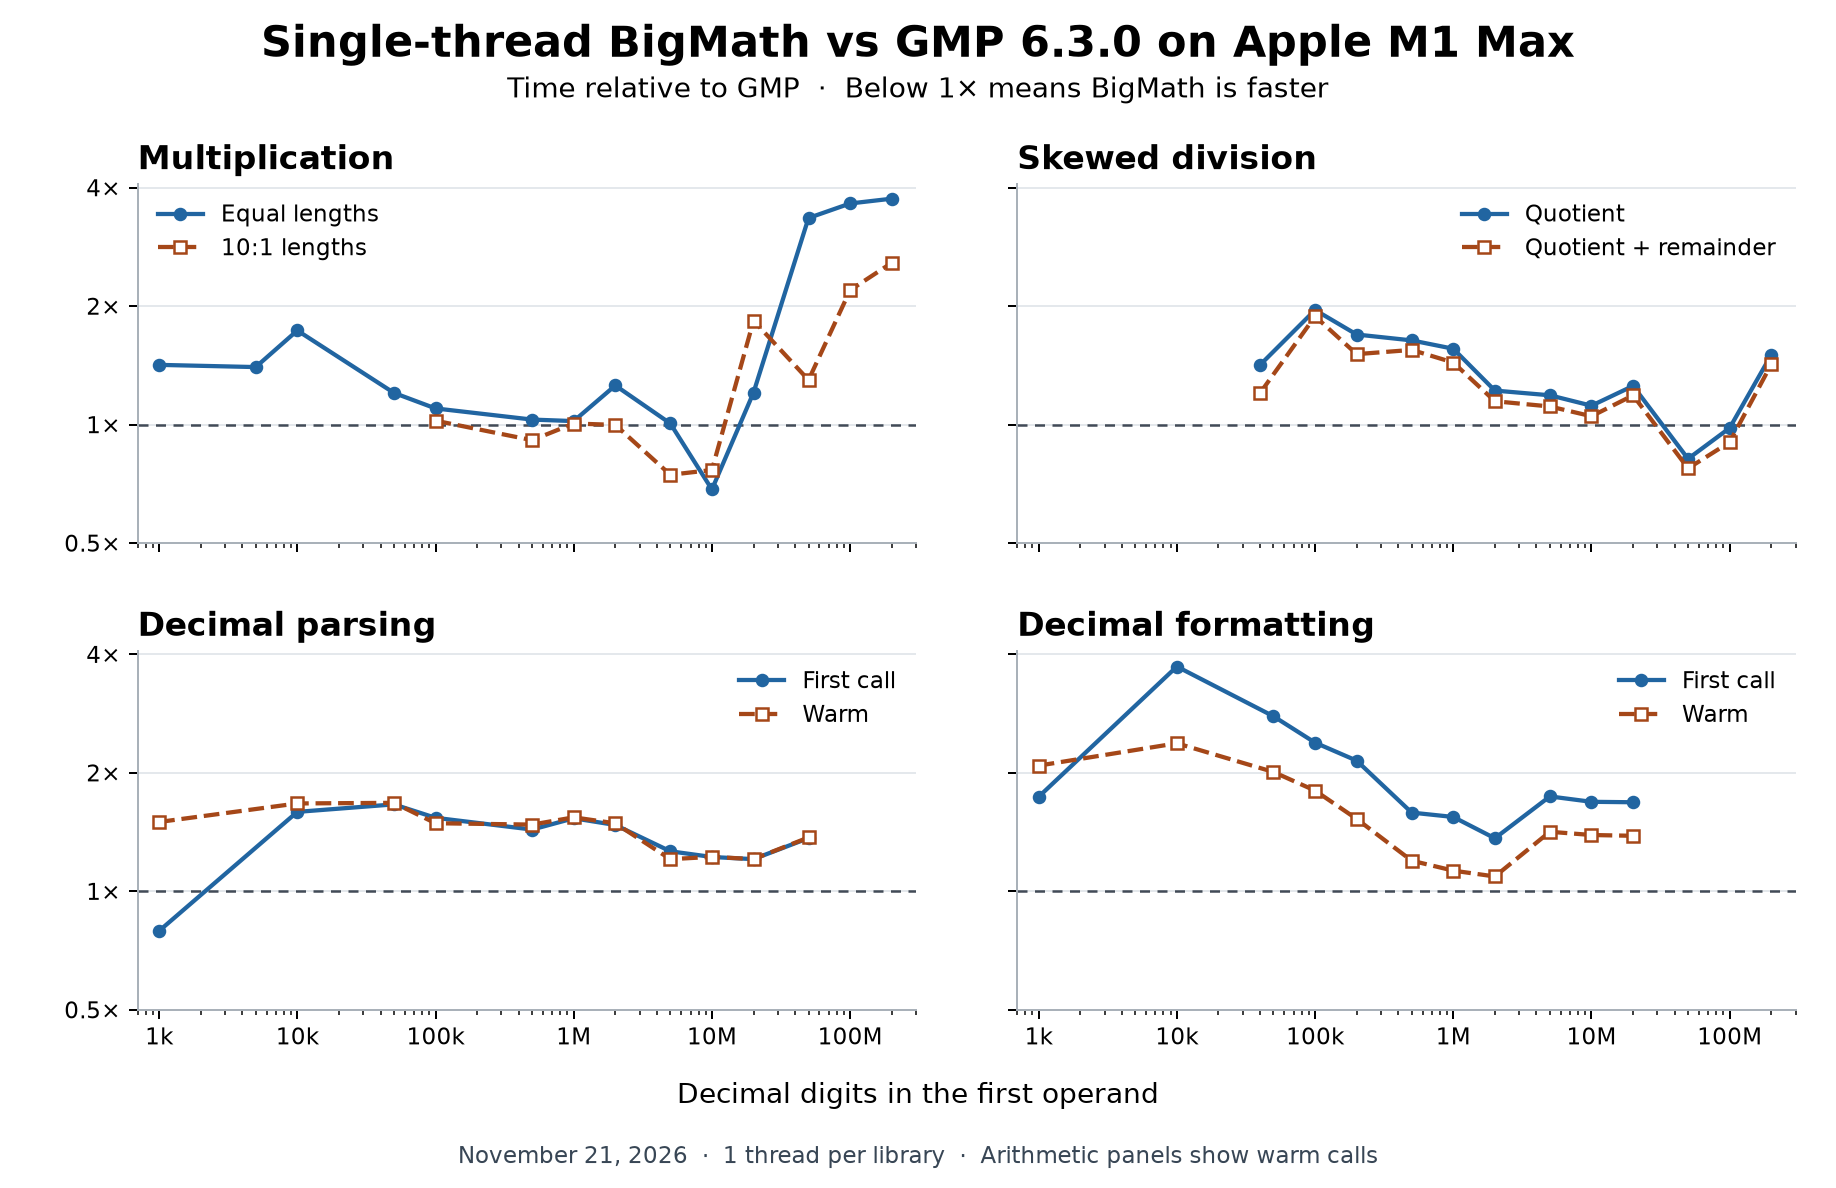
\includegraphics[width=\textwidth]{../images/bigmath_vs_gmp_single_thread.png}
\caption{Single-threaded BigMath time divided by single-threaded GMP time (below 1 means BigMath
was faster). From \file{docs/images/}, generated from the November 2026 benchmark run.}
\end{figure}

\begin{figure}[ht]
\centering
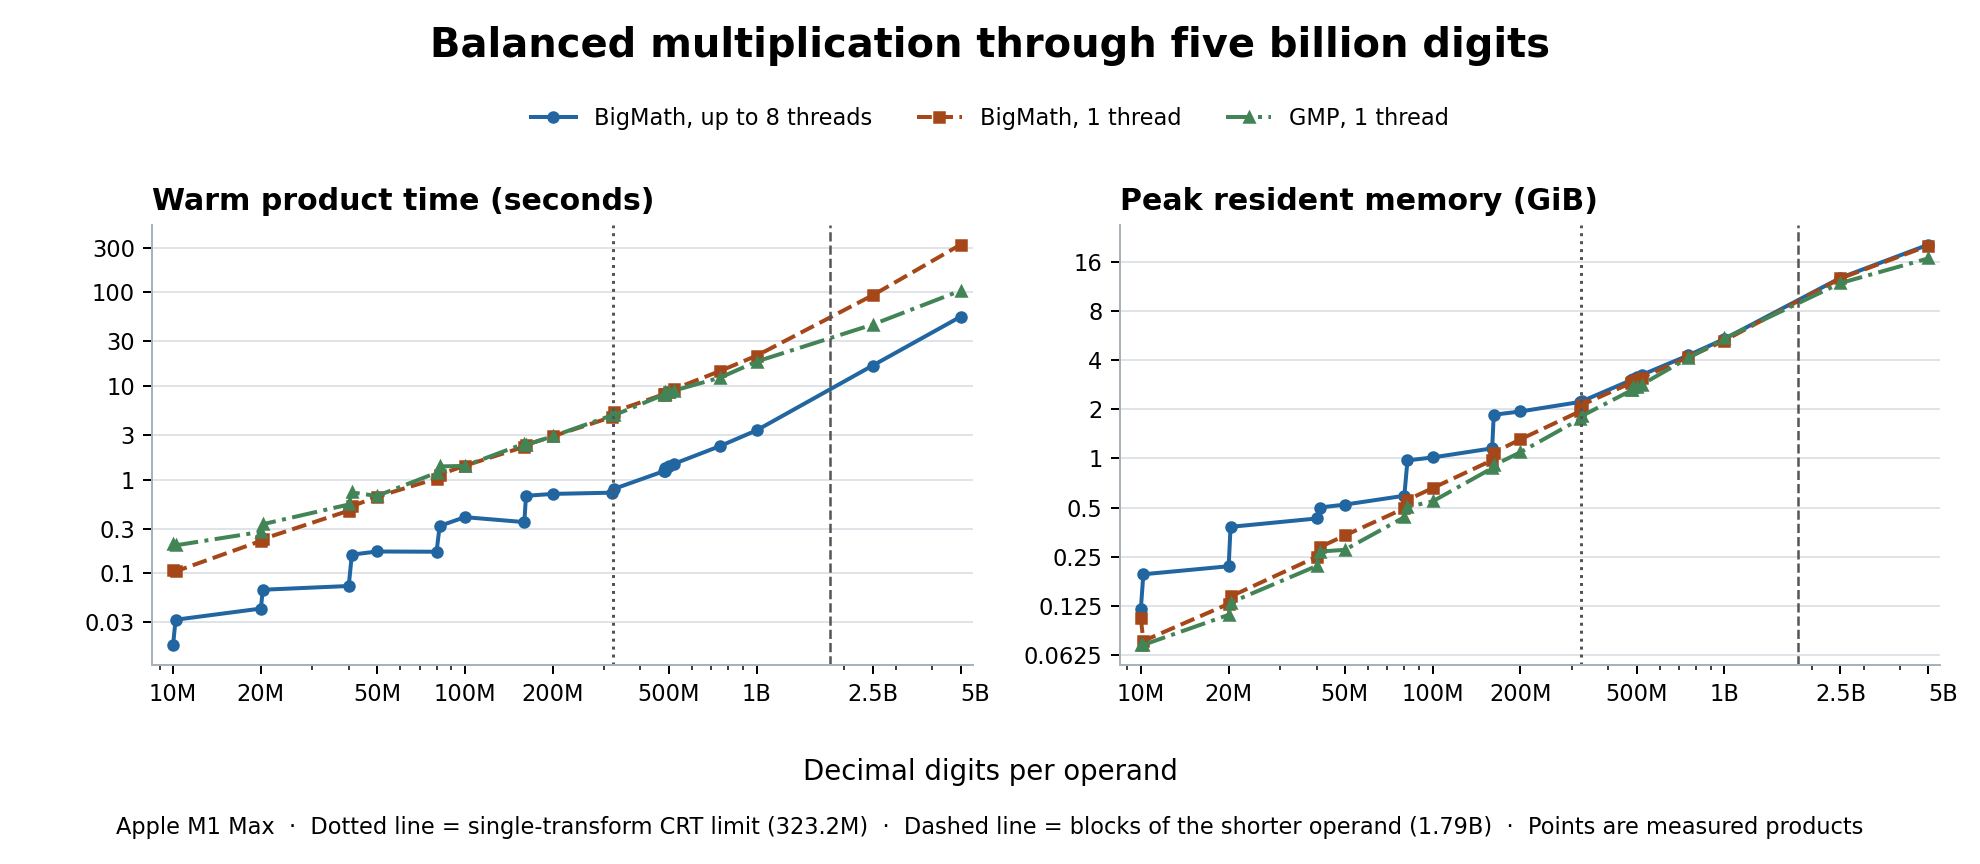
\includegraphics[width=\textwidth]{../images/bigmath_vs_gmp_large_products.png}
\caption{Fresh-process measurements through one billion decimal digits per operand.
The dotted line marks the largest single CRT transform. Products above it accumulate
multiple block products. Each point reports one warm multiplication and the process
peak through that call.}
\end{figure}

\section{Choosing the right call}

\begin{center}
\small
\renewcommand{\arraystretch}{1.25}
\begin{tabularx}{\textwidth}{lX}
\toprule
you want & use \\
\midrule
$a \times b$ & \code{a * b}. The dispatcher picks the method. \\
$a^2$ & \code{a * a} with the \emph{same object} on both sides: the library notices and squares. \\
many products with one fixed large factor & \code{PrepareMultiplication(a, maxOtherLimbs)} (\cref{ch:ntt}). \\
quotient only & \code{a / b}; much faster than \code{DivideAndRemainder} when the quotient is
               shorter than the divisor (\cref{sec:toplimbs}). \\
quotient and remainder & \code{DivideAndRemainder(a, b)}, one division for both. \\
many divisions by one divisor & \code{CacheDivision(b)} (\cref{sec:cached}). \\
division by a small constant & the \code{uint64\_t} overloads: \code{a / 10}, \code{a \% 10}. \\
text in / out & \code{BigIntegerBuilder::From(str)}, \code{ToString(x)}; the second call of a similar size is much faster than the first. \\
\bottomrule
\end{tabularx}
\end{center}

\section{Build options that change algorithms}

\begin{center}
\small
\begin{tabularx}{\textwidth}{lX}
\toprule
option & effect \\
\midrule
\code{-DBIGMATH\_USE\_THREADS=0} & no thread pool, no pthread dependency; every pool-dependent
                                   choice uses its ``cold'' threshold. \\
\code{-DBIGMATH\_MAX\_THREADS=N} & cap the pool at $N$ threads (default 8). \\
\code{-DBIGMATH\_POOL\_SPIN\_US=0} & idle workers sleep immediately: least idle CPU, slower
                                   bursts. \\
\code{-DBIGMATH\_NTT\_CRT=0} & single-prime (Goldilocks) NTT instead of three primes. Slower;
                              for comparison or unusual targets. \\
\code{-DBIGMATH\_NEON=0} & disable the ARM vector butterflies. \\
\code{-DBIGMATH\_LIMB\_64=0} & the legacy 32-bit-values-in-64-bit-slots layout; roughly 2$\times$
                              slower; for comparison. \\
any \code{-DBIGMATH\_*\_THRESHOLD=}$n$ & move a switch point (\cref{app:ref}). \\
\bottomrule
\end{tabularx}
\end{center}

Threshold overrides must be in effect when the \emph{library} is compiled (pass them through
\code{CMAKE\_CXX\_FLAGS}), because the dispatchers are compiled into \file{libbigmath.a}.

\section{Tuning for your machine}

The shipped thresholds were measured on an Apple M1 Max. On a different processor the crossovers
move, usually by tens of percent, not by factors. To measure your own:

\begin{lstlisting}[language=bash]
cmake -S . -B build -DCMAKE_BUILD_TYPE=Release
cmake --build build --target dispatch_tuner -j
./build/dispatch_tuner --full --emit-header \
    include/biginteger/build/platform/<os>-<arch>-<compiler>.h
\end{lstlisting}

The generated header is picked up automatically for that OS, architecture and compiler
(\file{docs/PLATFORM\_TUNING.md}). Precedence: command-line \code{-D} first, then the platform
profile, then the defaults in \file{DispatchThresholds.h}.

\section{Checking correctness after a change}

All algorithms are cross-checked against each other:

\begin{itemize}
  \item \code{mult\_correctness} multiplies with every method and compares limb for limb against
        schoolbook;
  \item \code{div\_correctness} runs every division algorithm, compares against reference
        implementations, and checks $q \cdot b + r = a$ and $0 \le r < b$ on every result;
  \item unit tests pin details such as the reciprocal's error bound, the zero-fallback guarantee
        of Newton division, and NTT layers against a plain radix-2 transform.
\end{itemize}

Run \code{ctest --output-on-failure} in the build directory after changing a threshold or an
algorithm. Passing means the new path agrees with an independent reference path, not just that it
ran.

\chapter{Design decisions and roads not taken}
\label{ch:decisions}

A library is shaped as much by what it leaves out as by what it includes. Each item below was
tried or seriously considered, and each has a concrete reason for its current status. The full
records are in \file{docs/MULTIPLICATION.md}, \file{docs/DIVISION.md} and
\file{docs/STRING\_CONVERSION.md}.

\section{Principles that recur}

\begin{enumerate}
  \item \textbf{Measure end to end, on the shapes that really occur.} Microbenchmarks of one
        algorithm in isolation repeatedly gave wrong crossovers: they missed setup costs, the
        pool's sleep state, or lopsided shapes. The thresholds come from timing the dispatcher's
        actual choices over grids of sizes and shapes.
  \item \textbf{Re-measure when a building block changes.} Faster kernels moved the Karatsuba
        leaf from 48 to 24 limbs; faster NTT butterflies retired the Toom-3 band and moved the
        NTT entry from 2560 to 320 limbs per operand. A threshold is only correct for the code it
        was measured with.
  \item \textbf{Change the dependency structure, not the instruction count.} The biggest
        small-size gains (two carry chains, fused NTT layers, interleaved twiddle tables, fused
        pointwise products) came from shortening dependency chains and memory passes.
  \item \textbf{Build big algorithms on the dispatcher.} Division and conversion ask
        \code{Multiply} for their products, so every multiplication improvement propagates.
  \item \textbf{Silent slow paths are bugs.} A correct-but-quadratic fallback is invisible to
        correctness tests, so fallbacks are counted and tested for (\cref{sec:newton}).
\end{enumerate}

\section{Rejected or retired}

\begin{description}[leftmargin=0pt,style=nextline,itemsep=6pt]
  \item[Schönhage--Strassen multiplication]
        A parameter sweep found no winning size band for the single-level implementation
        considered here. Each three-prime NTT block accepts up to $2^{26}$ coefficients,
        about 323 million digits per balanced operand. Further convolution residues of that
        length extend one product to about 1.79 billion digits per operand before block
        accumulation. Factoring the cross-twiddles and
        distributing matrix tiles across the pool reduced its cost within that range
        (\cref{sec:mfa,sec:nttthreads}). Measured times appear in \cref{ch:practice}.
  \item[Toom-3 as a top-level band]
        Once a separate band between Karatsuba and NTT (total 2560--5120 limbs). The vectorized NTT
        overtook it everywhere, so the band was retired. Toom-3 now lives inside the Karatsuba
        recursion instead (\cref{sec:toom}).
  \item[Toom-4 and Toom-5]
        Toom-4 is implemented but off: no gain on the M1 before the NTT starts. Toom-5 was
        3 times slower than Karatsuba at its first active size (512 limbs): its evaluation and
        interpolation cost more than the multiplications they save.
  \item[Two-row unrolled schoolbook]
        Measured flat (\cref{sec:flagchain}): it kept the limb-sized carry chain.
  \item[Barrett reduction for the NTT primes]
        Slower than the compiler's own code for division by a constant in this loop. Shoup's
        method (precomputed per twiddle) replaced both.
  \item[Montgomery reduction for the Goldilocks prime]
        That prime already has a special-form reduction of a few additions; Montgomery would only
        add conversions.
  \item[Short (high-half-only) products in Newton division]
        Implemented exactly and measured flat. At the sizes where Newton runs, products go through
        the NTT, where computing ``half a product'' as two smaller products costs about the same as
        one full product. Shortening the \emph{transform} (wrap-around products) worked instead
        (\cref{sec:wrap}).
  \item[Reusing a prepared transform inside Newton chunks]
        Cut the number of transforms but not the wall-clock time: the three primes already run in
        parallel, so fewer transforms did not shorten the critical path.
  \item[Splitting decimal conversion at powers $10^{18 \cdot 2^i}$]
        Unbalanced splits made it slower than the quadratic method (\cref{ch:conv}).
  \item[Per-layer threading of the NTT]
        Starting threads for every butterfly layer spent most of its time in synchronization.
        Coarse units (whole transforms, or large row ranges) replaced it.
  \item[Profile-guided optimization]
        No measurable change: the hot loops are already fully inlined and unrolled.
  \item[Storing numbers in base $10^{18}$]
        Would make printing trivial and all arithmetic slower; arithmetic dominates real work.
\end{description}

\section{Open opportunities}

The project's notes name these as the most promising remaining directions:

\begin{itemize}
  \item a half-size reciprocal with two quotient blocks for divisions of ratio about 2 (the shape
        of GMP's \code{mu\_div});
  \item block-recursive (Mulders) division and Schönhage's subquadratic GCD, if a workload needs
        them;
  \item removing the power-of-two staircase above $2^{20}$ coefficients in threaded builds.
\end{itemize}


\appendix
\chapter{Reference}
\label{app:ref}

\section{Every switch point}

All values are for the default build (64-bit limbs, three-prime NTT, threads on). Each is a
preprocessor macro that can be overridden with \code{-D} when compiling the library. Canonical
defaults are in \file{include/biginteger/build/DispatchThresholds.h} unless noted.

\subsection*{Multiplication and squaring}

\begin{longtable}{>{\raggedright\arraybackslash}p{0.5\textwidth}r>{\raggedright\arraybackslash}p{0.3\textwidth}}
\toprule
macro & default & meaning \\
\midrule
\endhead
\code{BIGMATH\_SMALL\_OPS\_MAX\_LIMBS} & 16 & stack-buffer path in the operators (\file{ops/SmallOps.h}) \\
\code{BIGMATH\_INLINE\_LIMBS} & 4 & values stored inside the object (\file{BigInteger.h}) \\
\code{BIGMATH\_CLASSIC\_MULTIPLICATION\_THRESHOLD} & 56 & schoolbook if $n_a + n_b \le$ this \\
\code{BIGMATH\_CLASSIC\_MIN\_LIMB\_THRESHOLD} & 24 & schoolbook if $\min(n_a,n_b) \le$ this \\
\code{BIGMATH\_KARATSUBA\_THRESHOLD} & 24 & Karatsuba leaf size (\file{KaratsubaMultiplication.h}) \\
\code{BIGMATH\_MUL\_TOOM33\_THRESHOLD} & 168 & Toom-3 split inside Karatsuba from this size \\
\code{BIGMATH\_MUL\_TOOM44\_THRESHOLD} & $10^6$ & Toom-4 split (effectively off) \\
\code{BIGMATH\_NTT\_MULTIPLICATION\_THRESHOLD} & 640 & NTT needs $n_a + n_b \ge$ this \\
\code{BIGMATH\_NTT\_MIN\_LIMB\_THRESHOLD} & 64 & NTT needs $\min(n_a,n_b) \ge$ this \\
\code{BIGMATH\_NTT\_AREA\_THRESHOLD} & 96\,000 & NTT needs $n_a n_b \ge$ this (warm pool) \\
\code{BIGMATH\_NTT\_COLD\_AREA\_THRESHOLD} & 262\,144 & NTT regardless of pool from this area \\
\code{BIGMATH\_SMALL\_SELF\_SQUARE\_MAX} & 319 & \code{x*x} goes to the square dispatcher up to this \\
\code{BIGMATH\_KARATSUBA\_SQUARE\_THRESHOLD} & 48 & schoolbook square below this (\file{KaratsubaSquare.h}) \\
\code{BIGMATH\_SQR\_TOOM3\_THRESHOLD} & 160 & Toom-3 split for squares \\
\code{BIGMATH\_NTT\_SQUARE\_THRESHOLD} & 352 & NTT square from this size (warm) \\
\code{BIGMATH\_NTT\_SQUARE\_COLD\_THRESHOLD} & 608 & NTT square regardless of pool \\
\code{BIGMATH\_NTT\_CRT\_THRESHOLD} & 256 & three-prime NTT vs Goldilocks (always three-prime in practice) \\
\code{BIGMATH\_NTT\_MFA\_THRESHOLD} & $2^{20}$ & matrix (six-step) method from this transform length \\
\code{BIGMATH\_NTT\_MFA\_LEAF} & $2^{13}$ & longest short transform in the matrix method \\
\code{BIGMATH\_NTT\_TRUNC\_MIN} / \code{\_MAX} & 2048 / $2^{20}$ & range of $H$ for the $H+L$ scheme \\
\code{BIGMATH\_NTT\_TRUNC\_SERIAL\_MAX} & $2^{25}$ & $H + L$ upper limit with one thread \\
\code{BIGMATH\_NTT\_PARALLEL\_MIN} & 2048 & smaller transforms run on the calling thread \\
\code{BIGMATH\_NTT\_FINALIZE\_PARALLEL\_MIN} & 4096 & carry pass split across threads from this many limbs \\
\bottomrule
\end{longtable}

\subsection*{Division}

\begin{longtable}{>{\raggedright\arraybackslash}p{0.5\textwidth}r>{\raggedright\arraybackslash}p{0.3\textwidth}}
\toprule
macro & default & meaning \\
\midrule
\endhead
\code{BIGMATH\_DIV\_BZ\_MIN\_B} & 96 & Algorithm D below this divisor length \\
\code{BIGMATH\_DIV\_NEWTON\_MIN\_B} & 1536 & Newton for ratio $\ge 2$ from this divisor length \\
\code{BIGMATH\_DIV\_NEWTON\_SKEW\_MIN\_B} & 768 & \ldots or from this length when ratio $\ge$ 3 \\
\code{BIGMATH\_DIV\_NEWTON\_SKEW\_RATIO} & 3 & the ratio for the line above \\
\code{BIGMATH\_DIV\_NEWTON\_NEAR2\_MIN\_B} & 3072 & Newton for ratio in $[7/4, 2)$ from this length \\
\code{BIGMATH\_DIV\_QSIZED\_MIN\_QUOTIENT} & 3072 & quotient-sized division from this quotient length \\
\code{BIGMATH\_DC\_DIV\_THRESHOLD} & 64 & Burnikel--Ziegler base case (\file{BurnikelZieglerDivision.h}) \\
\code{BIGMATH\_NEWTON\_SCHOOLBOOK\_HEAD} & 32 & short leading Newton blocks use Algorithm D \\
\code{BIGMATH\_CYCLIC\_NTT\_THRESHOLD} & 1280 & smallest wrap-around (mod $B^L-1$) product inside Newton \\
\bottomrule
\end{longtable}

\subsection*{Decimal conversion and threads}

\begin{longtable}{>{\raggedright\arraybackslash}p{0.5\textwidth}r>{\raggedright\arraybackslash}p{0.3\textwidth}}
\toprule
macro & default & meaning \\
\midrule
\endhead
\code{BIGMATH\_PARSE\_DC\_THRESHOLD} & 2048 & digits; linear parse up to this (\file{Parser.h}) \\
\code{BIGMATH\_TOSTR\_DC\_THRESHOLD} & 1024 & digits; linear print below this \\
\code{BIGMATH\_TOSTR\_NEWTON\_MIN\_DIGITS} & 13\,000 & cached reciprocal for print levels from here (1 thread) \\
\code{BIGMATH\_TOSTR\_NEWTON\_MIN\_DIGITS\_THREADED} & 6\,500 & same, with a multi-thread pool \\
\code{BIGMATH\_PARSE\_PARALLEL\_THRESHOLD} & 100\,000 & 8-way parallel parse from here \\
\code{BIGMATH\_TOSTR\_PARALLEL\_THRESHOLD} & 100\,000 & 8-way parallel print from here \\
\code{BIGMATH\_USE\_THREADS} & 1 & thread pool on/off \\
\code{BIGMATH\_MAX\_THREADS} & 8 & pool size cap \\
\code{BIGMATH\_POOL\_SPIN\_US} & 100 & \textmu s an idle worker spins before sleeping \\
\bottomrule
\end{longtable}

\section{Costs at a glance}

\begin{center}
\footnotesize
\begin{tabular}{lll}
\toprule
algorithm & cost for $n$-limb inputs & where in the code \\
\midrule
schoolbook multiply & $n^2$ & \file{ClassicMultiplication.h}, \file{LimbKernels.h} \\
Karatsuba & $n^{1.585}$ & \file{KaratsubaMultiplication.h} \\
Toom-3 & $n^{1.465}$ & \file{ToomKernels.h} \\
NTT (three primes) & $n \log n$ & \file{NTTMultiplicationCrt.h} \\
short division & $n$ & \file{ClassicDivision.h} \\
Algorithm D & $(n_a - n_b) \cdot n_b$ & \file{FastDivision.h} \\
Burnikel--Ziegler & $\M(n)\log n$ & \file{BurnikelZieglerDivision.h} \\
Newton & a few $\M(n)$ & \file{NewtonDivision.h} \\
parse / print (divide and conquer) & $\M(n)\log n$ & \file{src/common/Parser.cpp} \\
\bottomrule
\end{tabular}
\end{center}

\section{Further reading}

\begin{itemize}
  \item D.~E. Knuth, \emph{The Art of Computer Programming}, Vol.~2, §4.3: classical multiple-precision
        arithmetic and Algorithm D.
  \item R.~P. Brent and P.~Zimmermann, \emph{Modern Computer Arithmetic}, Cambridge University Press,
        2010: Karatsuba, Toom-Cook, FFT multiplication, Newton division, base conversion.
  \item C.~Burnikel and J.~Ziegler, ``Fast Recursive Division'', MPI-I-98-1-022, 1998.
  \item N.~Möller and T.~Granlund, ``Improved Division by Invariant Integers'', \emph{IEEE Transactions on
        Computers} 60(2), 2011.
  \item M.~Bodrato, ``Towards Optimal Toom-Cook Multiplication for Univariate and Multivariate
        Polynomials in Characteristic 2 and 0'', WAIFI 2007.
  \item V.~Shoup, NTL library: precomputed-quotient modular multiplication.
  \item D.~H. Bailey, ``FFTs in External or Hierarchical Memory'', \emph{J. Supercomputing} 4, 1990:
        the six-step FFT.
  \item The library's own technical notes, with full measurement history:
        \file{docs/MULTIPLICATION.md}, \file{docs/DIVISION.md}, \file{docs/STRING\_CONVERSION.md},
        \file{docs/BASE.md}, \file{docs/THREAD\_SAFETY.md}, \file{BENCHMARK.md}.
\end{itemize}


\end{document}
